% Copyright (C) 2014-2020 by Thomas Auzinger <thomas@auzinger.name>

\documentclass[draft,final]{vutinfth} % Remove option 'final' to obtain debug information.

% Load packages to allow in- and output of non-ASCII characters.
\usepackage{lmodern}        % Use an extension of the original Computer Modern font to minimize the use of bitmapped letters.
\usepackage[T1]{fontenc}    % Determines font encoding of the output. Font packages have to be included before this line.
\usepackage[utf8]{inputenc} % Determines encoding of the input. All input files have to use UTF8 encoding.

% Extended LaTeX functionality is enables by including packages with \usepackage{...}.
\usepackage{csquotes}   % used for easy quotes
\usepackage{amsmath}    % Extended typesetting of mathematical expression.
\usepackage{amssymb}    % Provides a multitude of mathematical symbols.
\usepackage{mathtools}  % Further extensions of mathematical typesetting.
\usepackage{microtype}  % Small-scale typographic enhancements.
\usepackage[inline]{enumitem} % User control over the layout of lists (itemize, enumerate, description).
\usepackage{multirow}   % Allows table elements to span several rows.
\usepackage{booktabs}   % Improves the typesettings of tables.
\usepackage{subcaption} % Allows the use of subfigures and enables their referencing.
\usepackage[ruled,linesnumbered,algochapter]{algorithm2e} % Enables the writing of pseudo code.
\usepackage[usenames,dvipsnames,table]{xcolor} % Allows the definition and use of colors. This package has to be included before tikz.
\usepackage{nag}       % Issues warnings when best practices in writing LaTeX documents are violated.
\usepackage{todonotes} % Provides tooltip-like todo notes.
\usepackage[square,numbers]{natbib}
\usepackage{hyperref}  % Enables cross linking in the electronic document version. This package has to be included second to last.
\usepackage{parskip}
\usepackage{rotating}
\usepackage{makecell}
\usepackage[acronym,toc]{glossaries} % Enables the generation of glossaries and lists fo acronyms. This package has to be included last.


% Define convenience functions to use the author name and the thesis title in the PDF document properties.
\newcommand{\authorname}{Lukas Weber} % The author name without titles.
\newcommand{\thesistitle}{Analysis, Design and Prototypical Implementation of a Serious Game to Aid in Speech Rehabilitation} % The title of the thesis. The English version should be used, if it exists.

% Set PDF document properties
\hypersetup{
    pdfpagelayout   = TwoPageRight,           % How the document is shown in PDF viewers (optional).
    linkbordercolor = {Melon},                % The color of the borders of boxes around crosslinks (optional).
    pdfauthor       = {\authorname},          % The author's name in the document properties (optional).
    pdftitle        = {\thesistitle},         % The document's title in the document properties (optional).
    pdfsubject      = {Subject},              % The document's subject in the document properties (optional).
    pdfkeywords     = {a, list, of, keywords} % The document's keywords in the document properties (optional).
}

\setpnumwidth{2.5em}        % Avoid overfull hboxes in the table of contents (see memoir manual).
\setsecnumdepth{subsection} % Enumerate subsections.

\nonzeroparskip             % Create space between paragraphs (optional).
\setlength{\parindent}{0pt} % Remove paragraph identation (optional).

\makeindex      % Use an optional index.
\makeglossaries % Use an optional glossary.
%\glstocfalse   % Remove the glossaries from the table of contents.

% Set persons with 4 arguments:
%  {title before name}{name}{title after name}{gender}
%  where both titles are optional (i.e. can be given as empty brackets {}).
\setauthor{}{\authorname}{Bsc.}{male}
\setauthorextra
\setadvisor{}{Thomas Grechenig}{}{male}

% For bachelor and master theses:
\setfirstassistant{Dipl.-Ing}{Christoph Aigner}{Bakk.techn.}{male}
%\setsecondassistant{Pretitle}{Forename Surname}{Posttitle}{male}
%\setthirdassistant{Pretitle}{Forename Surname}{Posttitle}{male}

% For dissertations:
\setfirstreviewer{Pretitle}{Forename Surname}{Posttitle}{male}
\setsecondreviewer{Pretitle}{Forename Surname}{Posttitle}{male}

% For dissertations at the PhD School and optionally for dissertations:
\setsecondadvisor{Pretitle}{Forename Surname}{Posttitle}{male} % Comment to remove.

% Required data.
\setregnumber{11909847}
\setdate{24}{01}{2025} % Set date with 3 arguments: {day}{month}{year}.
\settitle{\thesistitle}{{Analyse, Design und Prototypische Umsetzung eines Serious Game für therapeutische Zwecke in der Sprachtherapie.}} % Sets English and German version of the title (both can be English or German). If your title contains commas, enclose it with additional curvy brackets (i.e., {{your title}}) or define it as a macro as done with \thesistitle.
%\setsubtitle{Optional Subtitle of the Thesis}{Optionaler Untertitel der Arbeit} % Sets English and German version of the subtitle (both can be English or German).

% Select the thesis type: bachelor / master / doctor / phd-school.
% Bachelor:
%\setthesis{bachelor}
%
% Master:
\setthesis{master}
\setmasterdegree{dipl.} % dipl. / rer.nat. / rer.soc.oec. / master
%
% Doctor:
%\setthesis{doctor}
%\setdoctordegree{rer.soc.oec.}% rer.nat. / techn. / rer.soc.oec.
%
% Doctor at the PhD School
%\setthesis{phd-school} % Deactivate non-English title pages (see below)

% For bachelor and master:
\setcurriculum{Master programme Medical Informatics}{Masterstudium Medizinische Informatik} % Sets the English and German name of the curriculum.

% For dissertations at the PhD School:
\setfirstreviewerdata{Affiliation, Country}


\setsecondreviewerdata{Affiliation, Country}



\begin{document}

\frontmatter % Switches to roman numbering.
% The structure of the thesis has to conform to the guidelines at
%  https://informatics.tuwien.ac.at/study-services

\addtitlepage{naustrian} % German title page (not for dissertations at the PhD School).
\addtitlepage{english} % English title page.
\addinsotitlepage{naustrian}
\addstatementpage

\begin{danksagung*}
An dieser Stelle möchte ich mich bei allen bedanken, die mich nicht nur während der Verfassung dieser Masterarbeit, sondern auch während des gesamten Studiums unterstützt haben. Für das Mitwirken an dieser Arbeit möchte ich aber besonders Ao.Univ.Prof.Dipl.-Ing. Dr.techn. Thomas Grechenig, Dipl.-Ing. Christoph Aigner und Dipl.-Ing. Dr.techn René Baranyi aus dem COPA-Institut für ihre erstklassige Betreuung und wertvolles Feedback bedanken. Gleichzeitig möchte ich auch allen Testpersonen und Experten dafür danken, dass sie mir ihre Zeit zur Verfügung und mich in dieser Arbeit unterstützt haben. Zu guter Letzt ergeht mein Dank an meine Familie und Freunde, welche mich während des Studiums sowohl finanziell aber auch psychisch immer unterstützt haben. Ein besonderer Dank ergeht hierbei an meine langjährige Freundin, ohne die ich nicht annähernd so schnell im Studium vorangekokmmen wäre. \end{danksagung*}

\begin{acknowledgements*}
At this point, I would like to thank everyone who supported me by not only writing this thesis but also during the whole Master's program as well. For providing valuable information and constant feedback for this thesis, I would like to especially thank Ao.Univ.Prof.Dipl.-Ing. Dr.techn. Thomas Grechenig, Dipl.-Ing Christoph Aigner adn Dipl.-Ing. Dr.techn. René Baranyi from the COPA institute at TU Vienna. Also, I would like to thank all of my volunteers and experts who both invested time and effort to make this thesis possible. Last but not least I want to thank both my family and friends for supporting me during the whole duration of my study both financially and mentally. I would also like to especially thank my long-term girlfriend for always being there for me and without I would never have been able to progress through the Master's program as fast.
\end{acknowledgements*}

\begin{kurzfassung}
Die Fähigkeit zu sprechen ist ein essentieller Bestandteil der zwischenmenschlichen Kommunikation im Alltag. Obwohl die meisten Menschen diese Fähigkeit für selbstverständlich halten, so wird ihre Wichtigkeit erst wirklich klar, sobald sie beeinträchtig oder sogar verloren ist. Menschen mit Sprachbeeinträchtigungen haben oft mit erschwerten Bedingungen im Alltag zu kämpfen. Abhängig von der Art und Grad der Beeinträchtigungen leiden solche Menschen mehr oder weniger unter den folgen von sozialer Ausgeschlossenheit, erhöhtem Pflegebedarf oder psychischen Krankheiten wie Depression. \\
Die Logopädie ist eine medizinische Disziplin, welche genau solchen Menschen zu helfen versucht. Ähnlich wie bei einer Physiotherapie müssen Patienten verschiedene Übungen mit der LogopädIn bzw. alleine zu hause regelmäßig durchführen, um ihre sprachlichen Fähigkeiten langfristig zu verbessern. Dieser Prozess ist jedoch vor allem für Kinder, aber auch für erwachsene Patienten, mit sehr viel Arbeit und Disziplin verbunden, wodurch es oftmals zu Frequenzeinbußen der Therapiezeit kommt. Um dem entgegenzuwirken gibt es bereits einige Serious Games, welche den Therapieinhalt auf spielerische Weise präsentieren und somit ein Gefühl der Langeweile und Monotonie entgegenwirken. In den meisten Fällen müssen Patienten bei diesen Serious Games Wörter richtig aussprechen, um Fortschritte zu machen. Derzeitige Serious Games in diesem Bereich zeigen aber jedoch zumindest zwei große Lücken auf: Die Serious Games decken nur einen kleinen Teil des Rehabilitationsprozesses ab und die integrierte  Spracherkennungskomponente ist darauf trainiert worden, ganze Wörter anstatt einzelne Laute oder Silben zu erkennen. Gerade in der Sprachtherapie steht dies aber oftmals am Beginn der Therapie.\\
Diese Arbeit untersucht, welche Anforderungen ein Serious Game, welches für einen längeren Zeitraum im Therapieprozess eingesetzt werden kann, wichtig sind. Im Zuge der Arbeit wird ein solches Serious Game nicht nur theoretisch konzipiert, sondern auch gemeinsam mit einer Logopädin in einem User-Centered-Design (UCD) prototypisch umgesetzt. Ein weiterer Teil der Arbeit umfasst die Analyse, welche Metriken ein solches Serious Game einer LogopädIn liefern kann, damit Fortschritt des Patienten messbar gemacht werden kann. Dies ist gerade in der Logopädie nicht immer eindeutig zu beantworten. \\
Im Anschluss wird das Serious Game insgesamt 19 Teilnehmern, worunter drei LogopädInnen und eine PatientIn ist, zur Evaluation zur Verfügung gestellt. Das Ergebnis: Das entwickelte Serious Game bringt den gleichen subjektiven Lernerfolg, aber wirkt motivierender als reguläre Übungen. 
\end{kurzfassung}

\begin{abstract}
The ability to speak is an essential part of daily human communication. While most people perceive this ability to be given at any times, its importance becomes truly visible once it is impeded or even lost. Speech impeded patients are often faced with additional difficulties in their daily lives and, depending on the severity of the impediment, might even face social exclusion, need additional care or develop mental illnesses such as depression. \\
The field of speech therapy aims to aid precisely those people in improving their daily lives. Similar to physical therapy, patients have to exercise with the therapist and often also on their own at home to ensure significant progress. However, this constant exercise can often times be a daunting task and require strict discipline, especially for children. To somewhat mitigate this issue, Serious Games, which aim to provide speech exercises in a more engaging way, have been introduced. Players of those games have to often voice a certain word correctly in order to advance and thus practice while they play. However, research has concluded that all current Serious Games have at least two major issues that need addressing: For once, most Serious Games only tackle the word plane of the therapy process, meaning patients only have to issue whole words. Typically, however, therapy starts at correctly pronouncing single sounds before continuing to syllables and finally arriving at words. Thus, such Serious Games are only valid for a fracture of the therapy process. The second issue is that the voice recognition component used excels in detecting whole words, but has issues in correctly detecting single sounds or syllables which again makes the game unsuitable for most of the therapy process. \\
This thesis analyzes which requirements are necessary for developing a Serious Game that fills these two issues. During this thesis, a working prototype of such a Serious Game is implemented with the help of a local therapist's input. For that, a User-Centered-Design (UCD) approach is used to ensure high stakeholder satisfaction. Furthermore, this thesis also analyses whether and which data such a Serious Game can produce that can possibly aid the therapist in measuring patient progress or adapting the therapy process. \\
Last but not least, the prototypical Serious Game is distributed and evaluated regarding both subjective progress and subjective entertainment compared to classical therapy exercises. A total of 19 volunteers, three of which are therapists and one a patient, have been asked to play the Serious Game and afterwards provide feedback on it. As a result, the Serious Game scored similar regarding perceived subjective progress but exceeded regular exercises in terms of subjective entertainment value.
\end{abstract}

% Select the language of the thesis, e.g., english or naustrian.
\selectlanguage{english}

% Add a table of contents (toc).
\setcounter{secnumdepth}{3}
\setcounter{tocdepth}{3}
\tableofcontents % Starred version, i.e., \tableofcontents*, removes the self-entry.

% Switch to arabic numbering and start the enumeration of chapters in the table of content.
\mainmatter

\chapter{Introduction}
\label{chap:intro}
This thesis analyzes serious gaming for patients who lost or had their speech capabilities considerably impeded due to inner or outer causes (i.e., strokes or hereditary causes). The resulting speech impediment often results in a significant decrease in the patient's quality of life since the inability to speak also comes with an elevated need of care and dependability on others as well as social exclusion. Those issues have already been recognized and thus, therapeutic measurements have been developed and are constantly applied and improved on. However, as with all types of therapy, its true effectiveness can only be utilized if the patient's compliance supports it. In order to aid in this regard, Serious Games (i.e. games that promote therapy progression) have been introduced. In most of these Serious Games the patient has to issue voice commands in order to achieve a predetermined goal. However, current solutions are often faced with some drawbacks, the most prominent one being that exercising single vocals or syllables are not supported by any solution yet. In therapy, however, this is often considered to being the starting point for more severe cases. This makes current Serious Games only viable for a small fraction of the therapy process. This thesis proposes a prototypical implementation of a Serious Game that aims to overcome those shortcomings in order to aid such patients on their way to recovery. This Serious Game will furthermore also be evaluated regarding its effectiveness by conducting a field study.

This section starts with providing a brief summary regarding the problem domain of speech impediment Then, the expected results in the form of three research questions are presented. The next chapter then shortly describes the outline of this thesis and last but not least the summary concludes this section.
\section{Problem Description}
Since the beginning of human history, humans have been known to form social groups of like-minded individuals \cite{bentley2022prehistory}. Whether these groups were assembled due to providing better survival chances for the individual, or simply because having company is more enjoyable than living alone, finding a way of communicating with each other was and still is of most importance \cite{kelly2015knowledge}. While it is known that cavemen were drawing their stories on walls, it is more plausible to assume that most day-to-day interaction occurred on a verbal basis \cite{singleton2011communication}. 

This fact still holds true today, almost all human communication is based on verbal signals \cite{salim2023verbal}. Thus, as one can imagine, losing the ability to properly articulate one's opinions and wishes comes with a plethora of drawbacks such as social exclusion due to impeded communication, elevated dependability on peers and psychological issues such as depression \cite{hilari2010psychological}. While current literature is not definitive regarding the prevalence of speech impediments, estimations range from 0.82 to 4.4 individuals per 100.000 \cite{swain2018congenital, duffy2021primary}. However, it is likely that minor speech impediments like stuttering or impediments that might not even need therapy are a lot more common. The most common cause for severe speech impediments are previous strokes \cite{wu2020prevalence}, since often times crucial brain regions for speaking are affected. It is estimated that around 16.93\% of all stroke patients also suffer from Aphasia, which is often a sign of a neurodegenerative disease or trauma. Current trends seem to furthermore suggest that this metric seems to be increasing, most probably due to increased life expectancy.
To aid such patients, speech rehabilitation therapies are often applied in hopes to mitigate or at least improve on their vocal issues \cite{stahl2018efficacy}. Those therapies aim to improve the patient's vocal capabilities via constant training and specific speech exercises \cite{proestler2023}. Furthermore, therapy often includes exercises that include multiple senses (i.e., seeing, hearing, smelling,...) in order to promote neuroplasticity so that the functionality of damaged brain regions can be compensated by other ones. As with other types of rehabilitation, however, the path to success is a difficult one as much work and dedication from both the patient and the speech therapist is needed \cite{musicco2003early}.

Constant practice by the patient is crucial for the therapy's effectivity. Thus, patients are often advised to practice certain exercises at home on their own \cite{musicco2003early}. While effective, this approach can become tedious for some, especially for younger patients, resulting in lower exercise engagement and diminished results. To circumvent this issue, the concept of \emph{Serious Games} with the aim of making the learning process more enjoyable has been introduced \cite{lv2015game}. Most of these games aid the speech therapy process by including some kind of voice control capability instead of more classical input methods (i.e. keyboard or touchscreen), enabling the patient to simultaneously play the game as well as improve on their vocal skills.

However, introducing speech recognition within Serious Games with the specific goal to aid in speech therapy also comes with some issues which need to be addressed \cite{rohlfing2021hey}. As of now, no Serious Game implements a voice recognition software that was specifically designed to be used by speech-impeded users for rehabilitation. This results in the following two issues:
\begin{itemize}
\item The speech recognition software used excels in recognizing whole words or even sentences \cite{rohlfing2021hey}, but performs badly when tasked with interpreting single vocals or syllables. This issue stems from the way the recognition software is designed; usually, the user of the software speaks in whole sentences, not in single vocals. However, especially in more severe cases, practicing single vocals is often the starting point of rehabilitation.
\item As a consequence, there currently does not exist a Serious Game that covers multiple stages of therapy (i.e. vocal-, syllabic- and word stage), which can make it longer viable within the rehabilitation process.
\end{itemize}

Within this master thesis, a Serious Game that overcomes the mentioned issues with current implementations will be designed, developed, analyzed and evaluated. The game will be created in collaboration with the aid of a local speech therapist which provides both expert domain knowledge as well as recommendations regarding the game's design. The implementation process is going to follow a \emph{User-Centered Design} (UCD) approach, meaning the therapist's feedback is continuously integrated in order to ensure high user satisfaction. Nearing the end of this thesis, the game will also be distributed among a small group of volunteers consisting of therapists, patients and non-logopedical evaluators to gain both additional feedback as well as a final verdict regarding the game's perceived benefits. 
\section{Expected Results}
Through the process of developing and evaluating the Serious Game, the following research questions will be answered:

\begin{center}
\textbf{RQ1:} \textit{What are the requirements towards a Serious Game for speech rehabilitation that can be used across different steps of the rehabilitation process?}
\end{center} 

By addressing this research question, both the Serious Game developed within this thesis as well as similar future work benefit by having a clear view on what features have to be implemented for successfully introducing a beneficial game within the speech therapy process. This helps similar future research to compile a game that fulfills the basic requirements more quickly and thus allows for more resources to be allocated towards other issues.

\begin{center}
\textbf{RQ2:} \textit{What data within a Serious Game can be used to measure player progress and provide meaningful feedback for speech therapists?}
\end{center}

Since a Serious Game can only be seen as an additional tool for the therapist to use (rather than the game replacing classical speech therapy altogether), collecting meaningful data while the patient plays the game can further aid the therapist and thus improve the whole therapy progress. Such data includes common mispronunciations, level completion time or accuracy. Which type of information gathered does the therapist use to measure improvement?

\begin{center}
\textbf{RQ3:} \textit{Does the game provide a subjective benefit within the rehabilitation process for a predefined test group?}
\end{center}

As with classical therapy, a Serious Game can only aid the patient if it is actively played. Therefore, determining whether the game is both beneficial towards the therapy progress as well as entertaining enough to be continuously played is crucial. \\

\paragraph{Methodology Overview} To answer all three research questions, this thesis proposes a three-phase plan. The first phase covers a thorough literature research regarding the current state-of-the-art as well as an interview with a speech therapist to gather more domain knowledge. In the second phase, the game will be actively developed and a custom voice recognition model is trained. Last but not least, the third phase consists of collaboratively improving the Serious Game, taking the therapist's considerations into account, as well as conducting and evaluating a field study for the game. \\
Over the course of these three phases, the research questions will be answered. More specifically, for \emph{RQ1}, both a prototype of the Serious Game as well as a requirement catalog will be created. This process will take place across all three previously mentioned phases. \emph{RQ2} will be answered via interviewing the therapist during both phase 1 and 2. Finally, for \emph{RQ3}, a field study near the end of phase 3 will be conducted. For a more detailed structural overview please refer to chapter \ref{chap:methodoloy}.

\section{Structure}
This thesis consists of seven different chapters. Starting with chapter \ref{chap:intro}, an introduction regarding the thesis' problem domain and expected result is given. Next, chapter \ref{chap:theory} provides some theoretical background relevant for this thesis. This chapter provides various definitions of relevant concepts, including Serious Games and their rough classification, types of speech impediments, definition and classification of neural networks, voice recognition techniques and the User Centered Design (UCD) process. Next, chapter \ref{chap:state} will elaborate on the current State of the Art regarding speech rehabilitation games including a short comparison at the end. Furthermore, current voice recognition softwares and their advantages and drawbacks are also mentioned. Chapter \ref{chap:methodoloy} then briefly outlines the thesis' general course of action and also elaborates on how the three previously stated research questions are going to be answered. Next, chapter \ref{chap:results} presents the result of this thesis. This includes a description of various UCD-iterations, a requirement catalog for the game, a Use-Case diagram with detailed Use-Case descriptions, the game's architecture, known issues that still persist within the prototype and finally the evaluation of the game provided by a testing pool over the course of multiple months. Afterwards, the three previously mentioned research questions are answered in chapter \ref{chap:discussion} and the thesis concludes with chapter \ref{chap:conclusion} providing a conclusion and remarks regarding possible future work.

\section{Summary}
This chapter served as the introduction of this master thesis, and its most important statements are now summarized. \\
The ability to speak is an important aspect of day-to-day life as almost all interpersonal communication happens verbally. Thus, losing this ability severely impacts one's life in both physical (i.e. being more dependent on others) and psychological (i.e. less  socialization, developing depression, ...) aspects. While speech therapies aim to help such people to improve their lost verbal skills, it is often a hard and tedious process the patients have to undergo. The inclusion of Serious Games within the speech rehabilitation process aims to somewhat ease this process and make it more fun, thus hopefully improving therapy commitment by the patient and its success. Current Serious Games that were developed for speech therapy are, however, not without flaws; the main two issues that were identified are that none of the games cover multiple stages of the therapy process and thus only have limited usage, and that the voice recognition used within those games is not tailored to detect single sounds or syllables, thus heavily under-performing in these regards. These two issues are the main novelties that this master thesis aims to address within its own Serious Game. \\
More specifically, this thesis answers three different research questions that are centered around the development, usability and final evaluation of the developed Serious Game. Answering these questions include creating a requirement catalog, taking surveys, having interviews with a local therapist and finally developing the game itself.
\\

\chapter{Theoretical Background}
\label{chap:theory}
In order to develop an later on evaluate a Serious Game for medical purposes, prior knowledge from multiple disciplines is needed. This includes medical knowledge regarding speech impediment diseases, technical knowledge regarding both the voice recognition and artificial intelligence domain, as well as knowledge about the development process. Last but not least, it is also important to first define what exactly encompasses a Serious Game, meaning defining this term will also be done in this chapter.

The chapter starts with a definition and classification of Serious Games. Here, the focus will be on healthcare games as those are the most relevant for this thesis. Next, the two most common speech impediments are elaborated on. For each impediment, issues like affected neurological structures, progression, target demographic, therapeutic measurements and etiology are explained briefly. Furthermore, other less common or less impactful impediments are listed as well. Next, a short introduction to neural network, which is a subtype of artificial intelligence, is given. Topics like network components, node functions, network topology and the network learning process as well as some common variations will be discussed here. The next section will then focus more on the usage of AI within voice recognition context as well as highlight two additional steps that can improve neural network (and thus, in this case, voice recognition) output notably. The chapter then ends by introducing the rough idea of the UCD development process, which heavily incorporates stakeholders of the final product (in this case the game) in the development process.
\section{Serious Games}
As most are familiar with the term \emph{game}, which can be described as a recreational activity with fixed rules and predefined winning conditions that is mainly played for entertainment purposes \cite{smed2003towards}, a clear distinction between a game and a \emph{Serious Game} has to be made.

Additionally to providing entertainment, a Serious Game \cite{susi2007serious} also intends to benefit the player in some other way. These benefits can include aspects of, but are not limited to, workplace training, education or healthcare. The aim of such games is to improve the player's skills or knowledge while they are having fun doing so. Dörner et al. summarizes those benefits under the phrase \emph{characterizing goals} \cite{dorner2016contributing}, a term that is often used in literature.

\paragraph{Healthcare Games} are a subcategory of Serious Games that are of more importance in regard to this thesis. Those games aim to improve the physical or psychological state of its users, and can be roughly categorized into \cite{susi2007serious}:

\begin{itemize}
\item \textbf{Physical fitness} (exergaming): these Serious Games aim to promote healthy fitness habits. In most cases, the player can only play such games by moving around, thus exercising their body.%, but purely educational games which promote healthy lifestyle choices also fall under this category. 
Popular examples of such games include \emph{Wii Fit} \cite{nitz2010wii} or \emph{Dance Dance Revolution} \cite{trout2005using}. The usage of those games was met with a rising demand within the last few years \cite{santos2021active}. During the global COVID-19 pandemic, many children and adolescents were unable to exercise in school or within outer-school sport clubs due to the restrictions at hand. This led to a plethora of unwanted drawbacks, such as a reduction in energy-expensive activities and thus a rise in children's BMI within this time period. While the credibility of the BMI in regards to assessing an individual's health has taken a major hit in the last decade \cite{alpizar2020fat} as other, more sophisticated and indicative markers like the \emph{fat mass index} (FMI) arose, it can still provide valid information regarding obesity trends when applied not to the individual but a whole demographic. \\
Additionally, the lack of exercise also brings mental disorders to the table as well \cite{santos2021active}. During the COVID-19 pandemic, millions of children were diagnosed with anxiety disorders and depression due to isolation \cite{santos2021active}. While certainly not all of those diagnoses can be traced back to a lack of exercise, multiple studies have shown that regular exercise does have a positive impact on the mental state of its practitioners due to improving one's self-esteem and promoting socialization \cite{santos2021active,comeras2021effects}. 

\item \textbf{Education in health}: By educating its users about healthy habits (i.e. exercise, nutrition or mental health practices), such games also contribute to the user's longevity. An example for such a game is \emph{Hungry Red Planet}\cite{anderson2002hungry}. However, this category also encapsulates games that incorporate higher education relevant to medical students or staff. Around 26.1\% of all educational health games are tailored for this demographic \cite{sharifzadeh2020health}. Furthermore, with the advance and accessibility of technology, it is expected that more and more university-level lectures will include such games in the near future. To be truly accepted by a broader population, however, significant improvements have yet to occur. Most of the time, the development of such games is monopolized by technical team members, which often leads to aspects like user engagement and behavioral change drives lacking, thus making the games less entertaining than they could be \cite{sharifzadeh2020health}.

\item \textbf{Distraction therapy}: The aim of distraction therapy games is to alleviate the user's fear of an ongoing procedure by distracting them from it. Such games are more commonly used with children, but can also be applied to adult patients. However, even though a non-Serious Game could achieve the same result in this scenario, it is worth noting that games exist which were exactly developed for this purpose only. For example, \emph{Free Dive} \cite{dahlquist2008effects} was solely developed for this use. Within distraction therapy games, yet another distinction can be made depending on how the game distracts the user. This categorization consists of, but is not limited to, exergames, cognitive behavioral therapy games (CBT), biofeedback games, brain training games, and so on. However, a meta study \cite{abd2022effectiveness} concluded that the best statistically significant results regarding the effect of distraction games on the user's anxiety levels are achieved by \textbf{biofeedback and CBT games}, thus making the other types irrelevant for practical use as of now.

\item \textbf{Recovery and rehabilitation}: Describes games that play a more primary part within rehabilitation processes when compared to the other categories. The main defining characteristic of this category is that the user can only play the game in a way that directly correlates with the therapy measurements. For example, games using the Wii-Fit-Board can be used to re-learn lost sensorimotor capabilities. The game developed within this master thesis also falls under this category. \\
Current literature mainly focuses on post-stroke treatments for regaining motor capabilities within upper or lower limbs involving Serious Games. For this specific usage, however, Serious Games have been shown to benefit the patient more than classical therapy in regard to limb motor function and activity \cite{doumas2021serious}

\item \textbf{Training and simulation}: These games are used for safely training medical staff in order to improve performance \cite{michael2005serious}. An example for such a game is the 3D Anatomy Atlas \cite{anatomy3D} which lets the user easily dissect and view a 3D human model right on their phone.

\item \textbf{Diagnosis and treatment of mental illness}: This category is quite similar to the previous one. The main difference is the focus for the previous category lies on more on-hand training (i.e. simulation of surgery), whereas this category trains more the diagnostic and mental aspects of therapy \cite{michael2005serious}.

\item \textbf{Cognitive functioning}: Are games that improve the user's memory or logical capabilities. This category is again quite similar to \emph{Recovery and rehabilitation}, but the focus is more on mental therapy instead of physical.

\item \textbf{Control games}: This category describes games which provide the user with real-time information about his/her current physiological state (i.e. heart rate or body temperature). The goal is to teach better control of emotional states \cite{michael2005serious}.
\end{itemize}
To summarize, the field of Serious Games is more diverse than one might think at first glance. And while some games might be included in more than one category, it is still important that both the developers and therapists know in which category a game falls, as this vastly impacts the development process as well as its application.
\section{Speech Impediments}
While the result of all types of speech impediments are roughly the same (which can be described as the limited or nonexistent ability to speak) \cite{atakpaassessment}, distinctions are made between different types of impediments. Roughly speaking, there are two main categories of speech impediments\cite{proestler2023}: \emph{Apraxia} and \emph{Aphasia}:

\begin{figure}
\begin{center}
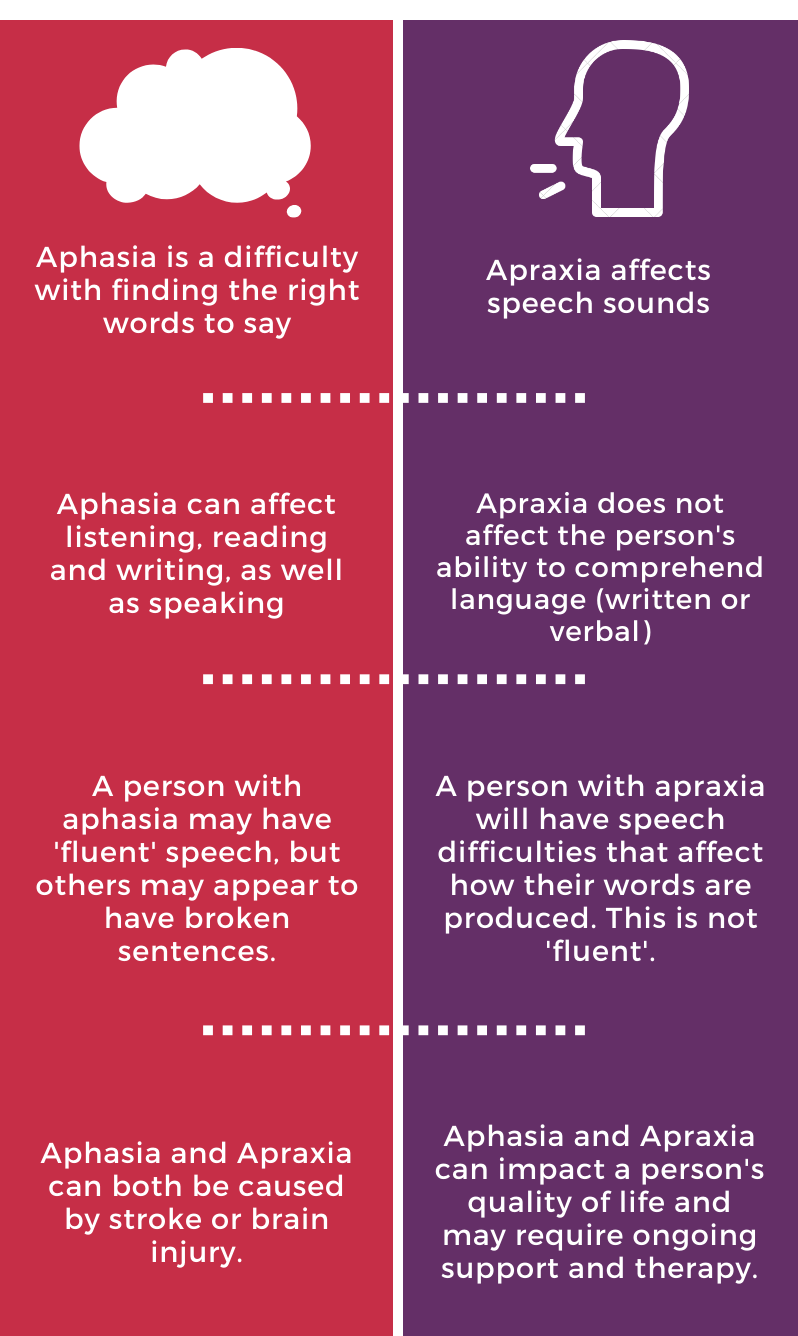
\includegraphics[scale=0.25]{ApraxiaAphasia}
\end{center}
\caption{The main symptomatic differences between Aphasia (left) and Apraxia (right).  \cite{ApraxiaAphasia}.}
\end{figure}
\subsection{Apraxia}
\label{sec:Apraxia}
Apraxia describes all speech impediments that stem from the inability to control the muscles used when speaking \cite{ogar2005apraxia}. Examples for such muscles are the various facial muscles, the tongue and muscles around the throat. As a result, patients who are affected from apraxia have trouble flexing and relaxing muscles, which leads to slower and less well-articulated speech. Furthermore, vocals are easier to pronounce since they can be elongated indefinitely, whereas consonants prove to be more difficult because of their short pronunciation. For example, in the word "boat", the vocal "a" can be stretched out ("a" becomes "aaa"), while the same cannot be done with the consonant "t" ("t" cannot become "ttt"), thus allowing for less time to correctly flexing and relaxing the muscles needed. 
\\ Apraxia can further be distinguished between \emph{phonetic} and \emph{prosodic-predominant} \cite{utianski2023update}. Phonetic-apraxic patients usually have sound distortions within their speech, i.e. single sounds are slurred, substituted or even added when not necessary. In contrast, prosodic-predominant-apraxic patients talk remarkably slower than usual and often include long breaks between syllables and words. In most cases, a mixture of both symptoms is present, but usually one prevails over the other.

\paragraph{Etiology} Apraxia is most commonly a result of some kind of brain impairment. Most frequently, damage to the left hemisphere due to a previous stroke or hemorrhage are the cause for apraxia. Other, less prevalent etiologies also include traumatic brain injuries, a building of an hematoma due to blood vessel malformation, or frontal cortical atrophy \cite{ziegler2008apraxia}.

\paragraph{Neuroanatomy} It is not yet entirely clear which dysfunctional brain region is responsible for apraxia \cite{ogar2005apraxia}. There are, however, some educated guesses, which include the left frontal and temporoparietal cortex \cite{mcneil2000apraxia}, the left superior anterior region of the insula \cite{dronkers1996new} and the left subcortical structures \cite{peach2004phonemic}. In all cases, the cells within those regions suffer from \emph{focal atrophy}, i.e., a reduced functionality capability.

\paragraph{Progression} In severe cases, apraxia can be classified as \emph{primary progressive apraxia of speech } (PPAOS) \cite{utianski2023update}. As the name suggests, the symptoms become more noticeable as time goes on. Additionally, patients with PPAOS also often suffer from aphasia later on. Furthermore, Bradykinesia (i.e., slower body-movement) and sensorimotor issues are also quite common, eventually binding the patient to a wheelchair \cite{utianski2023update}. In some cases, patients might even develop vertical supranuclear gaze palsy, which describes slow vertical movement of the eyes, or suffer from sleep disturbances or incontinence \cite{utianski2023update}.

\paragraph{Demographic} As of now, there is no formal study on how common apraxia is among the population. However, the prevalence has been estimated to be around 2 per 100,000 patients \cite{duffy2021primary}. If including patients that also suffer from a mild form of aphasia, this number increases to 4.4 per 100,000. The patients are usually between 30 and 90, with the majority being over 65 years of age. Furthermore, there could not be made any correlations between the patient's socioeconomic, educational or environmental background and the probability of suffering from apraxia. However, around 25\% of patients report having at least one distant family member that is affected by a neurodegenerative disease.

\paragraph{Therapy} There are some general guidelines for treating both apraxia and aphasia. Best results are achieved when multiple areas of the brain are stimulated, and therefore more cross-references between the regions are created. For example, in order to learn the word "key", the following cues can be used \cite{proestler2023}:
\begin{itemize}
\item \textbf{Vocal cues} (talking): By practicing the word "key", the patient improves its pronunciation.
\item \textbf{Visualization}: Seeing the key while practicing stimulates an additional brain area.
\item \textbf{Smell}: Identical to visualization, smelling the key also improves therapy success.
\item \textbf{Feeling}: Makes use of tactile brain components.
\item \textbf{Sound}: i.e., rattling the key.
\end{itemize}

For apraxic patients, it is additionally important to relearn the facial and oral expressions which are needed for communication \cite{ogar2005apraxia}. Issues like lip placement, tongue alignment and the opening of the jaw have to be practiced, mostly also by the patient alone at home. Depending on the patient, the exercises can be described formally (i.e., 'push tongue side to side') or figuratively (i.e., 'chewing a candy') \cite{proestler2023}.
\subsection{Aphasia}
\label{sec:Aphasia}
In contrast, aphasia is a purely neurological condition, as all muscles required for talking can be properly utilized. However, for those patients the concept of speech itself has been compromised \cite{clark2003aphasia}. Aphasic patients typically talk in a non-coherent way and have extended reaction time when asked questions. When they do speak, however, their words are clear to understand (even though they might lack some melodic nuanciations when compared to a healthy individual). Aphasia is often considered to be a consequence of strokes. As with apraxia, aphasia can again be further classified into \cite{ulugut2022natural}:
\begin{itemize}
\item \textbf{Semantic variant primary progressive aphasia (svPPA)}: Patients with svPPA have issues associating objects with their corresponding words, meaning they know the word but do not understand its meaning.
\item \textbf{Non-fluent/agrammatic variant PPA}: nfvPPA results in reduced speech speed and loss of grammar.
\item \textbf{Logopenic variant PPA}: lvPPA comes with word-finding difficulties and repetition problems. 
\end{itemize}

However, while helpful, this classification is far from extensive. It is estimated that around $1/3$ to $1/2$ of all PPA patients do not fall into one of these categories. Thus, the usage of a default classification called \emph{PPA mixed} is still widely used \cite{ulugut2022natural}.

\paragraph{Etiology} As with apraxia, the most common cause for aphasia is considered to be a previous stroke or hemorrhage. However, a traumatic brain injury can also cause aphasia in patients. Less common, but still present, is aphasia acquired due to building of brain tumors or infectious diseases like herpes, encephalitis or dementing diseases like Alzheimer's \cite{clark2003aphasia}.

\paragraph{Neuroanatomy} Similar to apraxia, it is not yet fully known which region of the brain is responsible for aphasia, but there are again some estimations. Aphasic patients often have lesions in the left persylvian cerebral cortex or damages in the inferior left frontal gyrus. \cite{clark2003aphasia}.

\paragraph{Progression} As the name suggests, PPA worsens over time. Depending on the additionally gained symptoms, a previously with PPA diagnosed patient might be either diagnosed with \emph{PPA-extended} or \emph{PPA-plus} \cite{ulugut2022natural}. PPA-extended means that the patient gains speech impediments that belong to another PPA subcategory than the one the patient was initially diagnosed with (i.e., a svPPA patient also gets grammatical issues). In contrast, PPA-plus describes the addition of other neurodegenerative symptoms altogether. These include, but are not limited to, global cognitive decline, memory deficits, executive dysfunction and visuospatial problems (i.e., the disability to correctly see and interpret one's surroundings) \cite{ulugut2022natural}.

\paragraph{Demographic} Since aphasia is most often caused by a previous stroke, almost all studies investigating its prevalence heavily focus on a limited demographic by only viewing stroke patients rather than making assumptions for the whole population. However, within this context, a study that elaborated on the prevalence of aphasia within patients who suffered a stroke between 2003 and 2014 \cite{wu2020prevalence} showed that around 16.93\% had aphasia. Those patients were statistically around 2.5 years older than the others and also slightly skewed toward female predominance. Furthermore, aphasic patients were more likely to be white and have an above-median income. Any aphasic patient was also more likely to suffer from additional conditions such as heart failure, depression and atrial fibrillation. \\
Last but not least, it is important to note that the prevalence of aphasia seems to be on the rise. While in 2003 only around 13.34\% suffered from this condition, this number rose to 21.94\% by 2014. The exact cause of this is still not certain, but increased life expectancy is likely to factor in this development as older people seem to be more prone to aphasia.

\paragraph{Therapy} The usage of a multitude of different cues as described above is even more important for aphasic patients. Typical therapy often relies heavily on auditory stimulation and an incremental learn approach; the patient first has to learn the meaning behind single words, which continuously evolves into reading whole short stories and answering questions about them \cite{proestler2023}.


Furthermore, if vocal communication is not an option any longer due to the severity of the disease, a suitable approach could be to introduce an alternative set of symbols (i.e. a custom alphabet) \cite{glass1973artificial}. For this case, a set of symbols which was originally intended to teach chimpanzees how to communicate has  been used for aphasic patients with notable success.

Lastly, the usage of pharmaceutics within speech therapy is under ongoing discussion \cite{raymer2001effects, sabe1995randomized,small1994pharmacotherapy}.
By ingesting various neurotransmitters, neuron activation of the affected brain regions should be promoted, thus reducing the symptoms of aphasia, However, no study has yet shown significant long-term benefits using a pharmaceutical approach.

\subsection{Other speech impediments}
While apraxia and aphasia are the most prevalent types of speech impediments therapists face, they are not the only ones. Below is a selection of other speech impediments, although not all of them require logopedical intervention to mitigate:

\begin{itemize}
\item \textbf{Stuttering} \cite{atakpaassessment, balaji2015speech}: Stuttering describes the inability to complete a specific word without repeating parts of it. Depending on the severity, this might occur on occasion when attempting to utter a more complex word, or it could happen more frequently, making it a serious condition that impacts daily communication. 

\item \textbf{Cluttering} \cite{balaji2015speech}: Cluttered speech is characterized by its speech speed being exceptionally fast or irregular. While many people speak fast naturally, one can only talk about cluttered speech when the talking speed extends so far that it becomes non-understandable to the majority of listeners.

\item \textbf{Articulation Errors} \cite{atakpaassessment}: Articulation errors occur when patients are unable to correctly pronounce certain phrases due to having issues in correctly placing their tongue within the mouth. The most prominent example of this is lisping, in which patients struggle to pronounce "s". While annoying, this impediment can be corrected via therapy, with the best results present in children \cite{proestler2023}.

\item \textbf{Esophageal voice} \cite{balaji2015speech}: An esophageal voice describes a speech pattern in which the muscles surrounding the esophagus vibrate more than normally. This occurs when the patient swallows air and then tries to speak. Such patients can only talk rather quietly and slowly as air has to be continuously swallowed in, which requires time. On the upside, learning to talk using this technique can actually improve one's voice capabilities if talking using the vocal cords is no longer an option due to accident or prior surgery.

\item \textbf{Anklyoglossia} \cite{atakpaassessment}: Also informally known as "tongue-tie", this impediment makes it more difficult for the patient to move his or her tongue, thus resulting in slurred speech.

\item \textbf{Selective mutism} \cite{atakpaassessment}: Selective mutism does not describe a physiological impediment, but rather a psychological one. When patients get too anxious due to being in an uncomfortable situation or place, they lose the ability to speak altogether. In this case, psychological therapy is more likely to be helpful than logopedical exercises \cite{proestler2023}.

\item \textbf{Dysarthria} \cite{balaji2015speech}: Dysarthria is a condition in which the muscles needed for speech do not act as intended. While this might sound similar to apraxia, there is one key difference: In apraxia, the brain has difficulties sending the correct signals to the otherwise functioning muscles, while dysarthric patients have the exact opposite problem, as their brain works as intended but the muscles themselves are faulty. Possible reasons for dysarthria include paralysis of the lips, tongue, jaw or larynx.
\end{itemize}

\section{Therapeutic Compliance}
As previously mentioned in section \ref{sec:Apraxia} and \ref{sec:Aphasia}, therapeutic measures to aid patients already exist and are applied in practice. However, even the best planned therapy executed by the most experienced therapist can only support improvement if the patient adheres to it for its whole duration \cite{dusing2001adverse}. Within healthcare this is known as \emph{compliance} or \emph{therapeutic compliance} and while almost all patients want to improve on their impeded capabilities, practice shows that only a fraction complies as recommended by their healthcare provider \cite{jin2008factors}. Depending on the type and duration of the therapy, number of compliant patients varies between 70\%-80\% for short-term therapies down to 20\%-30\% for lifestyle changes, i.e. changes that have to persist for the rest of the patient's life \cite{jin2008factors}.

Naturally, the question arises on why patients do not comply to their recommended therapy. It is fair to assume that every patient seeks to better himself, so why disregard a proven process prescribed by medical professionals? This exact question was asked by Jing et. al \cite{jin2008factors} who decided to conduct a meta study to identify the most commmon factors that lead to non-compliance. Those factors cover a multitude of categories, including patient-related factors like age, ethnicity and health literacy, therapy-related factors like treatment complexity, route of administration and side-effects, and social and economic factors like time commitment, therapy cost and social support. As a result, the study conducted that the most impactful factors are most likely to be therapy-related, meaning patients are more likely to comply if the therapy itself is more appealing to them. This statement also heavily supports this master thesis' aim of developing a Serious Game. 
Another study by Düsing \cite{dusing2001adverse} stated the most frequent reasons for noncompliance to be forgetfulness, severe side effects and lifestyle changes. While side effects can be most likely neglected for speech therapy, both forgetfulness and lifestyle changes do likely factor in. Again, however, Serious Games can aid in this regard by providing improved accessibility and accountability in the form of mobile games. \\
It is worth noting that the issue of therapeutic non-compliance is not limited to any special field of medicine but rather encompasses multiple types of therapy. A quite popular example of this are physical therapies \cite{campbell2001don}. Due to the long therapy process which often demands at-home exercises from patients, non-compliance is a serious issue. Other prominent examples would be asthma therapy \cite{cochrane2000inhaled}, therapy regarding osteoporosis \cite{siris2006adherence}, diabetes therapy \cite{garcia2013adherence} and many more. Campbell et al. \cite{campbell2001don} proposed a model of continued compliance for patients with knee issues, although the core idea can be applied for any kind of therapy (see Figure 2.2). The major factors within this model are:

\begin{itemize}
\item\textbf{Attitudes towards exercise}:  In order to ensure therapy compliance, patients have to both have a positive disposition towards the therapy as well as be willing to accommodate it into their everyday life.
\item\textbf{Perceived severity of (knee) symptoms}: Patients are more likely to comply to therapy if the symptoms of the underlying condition cause severe pain or highly impede a normal lifestyle.
\item\textbf{Ideas about the cause of the disease or injury (i.e. arthritis)}:  Patients need to know that active therapy aids their condition and that it is not solely caused by immutable factors like age, obesity or similar.
\item\textbf{Perceived effectiveness of the intervention}: If patients adhere to their therapies, improvements are more likely to follow. This creates a positive feedback loop in which the patient becomes more motivated to follow therapy and thus further improves on his or her condition.
\end{itemize}

\begin{figure}
\label{fig:compliance}
\begin{center}
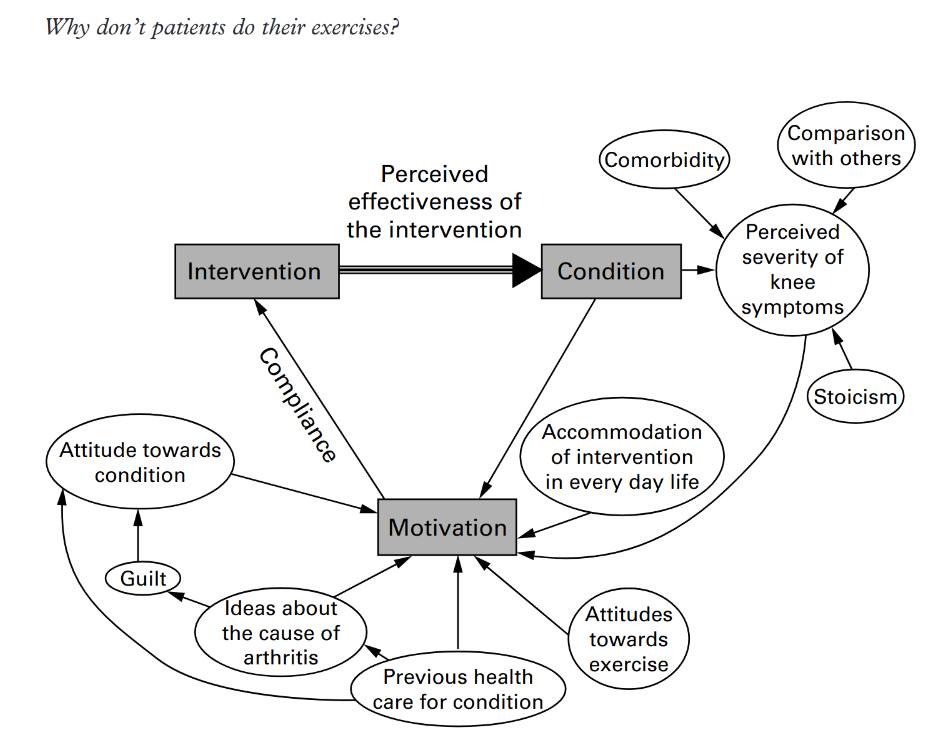
\includegraphics[scale=0.35]{compliance}
\end{center}
\caption{Model of continued compliance \cite{campbell2001don}.}
\end{figure}
\section{Neural Networks}
A neural network describes a machine learning technique which aims to simulate the functionality of the human brain \cite{suryadevara2021comprehensive}. Even though computers nowadays vastly outperform any human in regard to computation speed, they do lack behind in perceptual tasks such as image or speech recognition, with the latter being highly relevant for this thesis. Thus, in order to automate such tasks, the development of an \emph{artificial neural network} is of interest \cite{zou2009overview}. \\

\paragraph{The human brain} To understand how an artificial network operates, its real life model (the human brain) will be first inspected. The brain consists of billions of cells called \emph{neurons}, which are highly intertwined with each other \cite{shanmuganathan2016artificial}. Each neuron consists of a cell body or \emph{soma} which contains the nucleus of the cell, and \emph{axons} which are spread out and connect one cell with another one \cite{ariyo2024anatomy}. The connection between two cell's axons is called \emph{synapse} \cite{zou2009overview}. The actual communication between two cells occurs in the form of electrochemical signals travelling along the synapses \cite{ariyo2024anatomy}. Depending on the intensity of the signal and the synapse's individual threshold, the neighboring cell might be activated, thus again sending signals to its neighbors and so on. Depending on which cells are activated and which synapses are used for activation, a different output (i.e., action) is generated \cite{zou2009overview}.  
It is worth noting that in a biological neural network the activation of a neuron is not the only indicator for action. Additionally, the used synapse to activate the neuron also includes information, so does the timing of the activated synapse \cite{ariyo2024anatomy}. This is one reason on why biological neural networks can perform tasks like image recognition with a far smaller number of neurons than artificial neural networks can \cite{zou2009overview}.  

\begin{figure}
\begin{center}
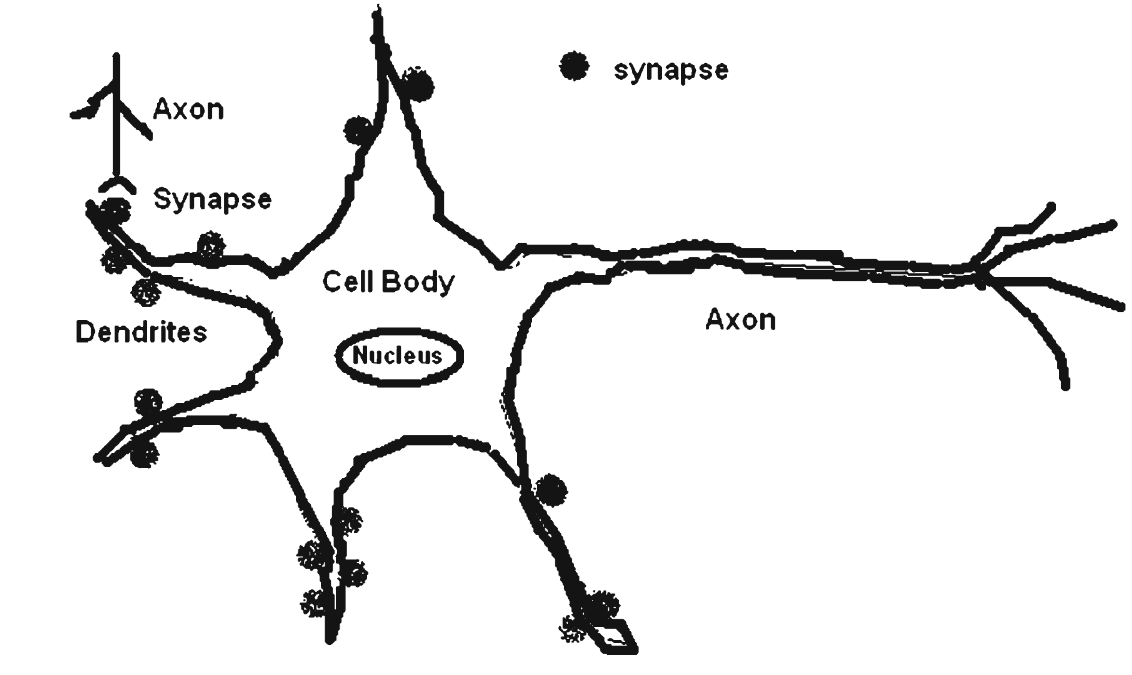
\includegraphics[scale=0.25]{Neuron}
\end{center}
\caption{The anatomy of a neuron \cite{zou2009overview}.}
\end{figure}

\paragraph{Artificial neural network} An artificial neural network (\emph{ANN} in short) is inspired by its biological counterpart; similar to the human brain, it also consists of many neurons (also called \emph{nodes}) and synapses (the link between nodes). Roughly speaking, a neural network consists of three main components: \emph{node character, network topology} and \emph{learning rules} \cite{zou2009overview}

\subparagraph{Node Character} The node character determines the structure of a single node within the network. This includes the number of inputs and outputs, as well as the \emph{activation function} (i.e., the logic determining whether a neuron fires a signal depending on its input) \cite{wu2018development}. Each input has furthermore a weight associated with it. The higher the weight, the "more important" a signal travelling through this input is regarded. When the weighted sum of all inputs of a neuron exceeds a predetermined threshold, the neuron fires a signal through its outputs to other neurons \cite{zou2009overview}. Mathematically, the relationship between input and output could be expressed like this \cite{mcculloch1943logical}:
\begin{center}
$y=f(\sum_{i=0}^n w_i x_i - T)$
\end{center}
where $y$ is the output, $w_i$ the weight of input $i$, $x_i$ determines whether input $i$ is activated and $T$ is the threshold value.\\
\begin{figure}
\begin{center}
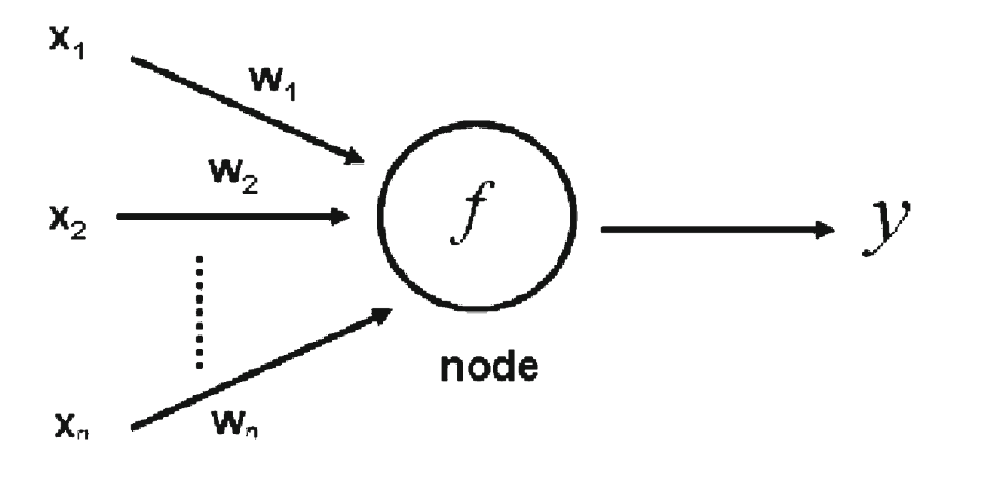
\includegraphics[scale=0.25]{Node}
\end{center}
\caption{A model of an artificial node with $x_i$ being the input, $w_i$ the weights, $f$ the activation function and $y$ the output \cite{zou2009overview}.}
\end{figure}

Furthermore, assuming the neuron fires due to sufficient input, the signal strength can also be altered by the activation function $f(x)$. The most common activation function is the \emph{binary step function}, which acts just as described above: if the input of the neuron is above a defined threshold, its output will be 1, otherwise 0. Some other, more complex functions include \cite{wang2020influence}:
\begin{itemize}
\item \textbf{Linear or identity function:} The identity function simply outputs its input and could therefore be considered a pseudo function \cite{kiaei2023active}: 

\begin{center}
$f(x)=x$
\end{center}

\item \textbf{Sigmoid function}: The sigmoid function is a non-linear function that was often used within the learning process of deep neural networks. Coincidentally, it also represents its biological counterpart more realistically than the previous versions. However, due to its shallow slope at both small and large inputs, which complicates the learning process due to less distinguishability, and its limitation to only output positive values, it is not considered best practice for today's standards. The function is defined as \cite{tsai2015hardware}
\begin{center}
$f(x)=\frac{1}{1+e^{-x}}$.
\end{center}

\item \textbf{Tanh function}: The tanh function is quite similar to the sigmoid function. The only difference is that this function allows for negative input as well, which in turn elevates the neuron's expressability. The formula of the function is \cite{tsai2015hardware}:
\begin{center}
$f(x)=\frac{1-e^{-2x}}{1+e^{-2x}}$
\end{center} 

\item \textbf{ReLu function}: Combining both the step function and identity function results in the ReLu function. The ReLu function is 0 for every negative value, and equal to the value otherwise. Due to its relative simplicity, this function is much more performant compared to other non-linear functions but comes at the cost of expressability for every value below 0. The function looks as follows \cite{bai2022relu}:
\begin{center}
$f(x)=max(0,x)$
\end{center}

As of now, ReLu functions are preferred within neural networks due to their advantageous performance. To counteract its drawbacks, various variations like the \emph{leaky ReLu} or \emph{Tanh-Relu} functions have been proposed \cite{bai2022relu}.

\item \textbf{Softplus function}: The softplus function could be considered to be a similar non-linear version of the identity function. This makes the function both harder to compute, as well as introduces a bias towards higher values. It is defined as \cite{zheng2015improving}:
\begin{center}
$f(x)=log(1+e^x)$
\end{center} 

\end{itemize}
\begin{figure}
\begin{center}
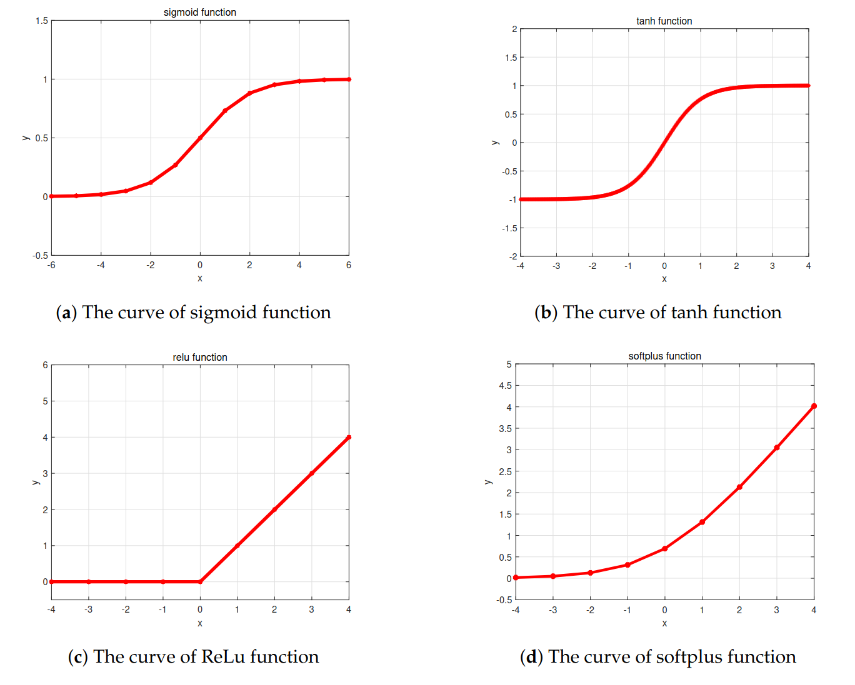
\includegraphics[scale=0.5]{ActivationFunctions}
\end{center}
\caption{Plots of the activation functions for sigmoid, tanh, ReLu and softplus functions \cite{wang2020influence}.}
\end{figure}
\subparagraph{Network Topology} The network topology describes how the neurons are organized within the neural network. Generally speaking, the neurons are sorted into \emph{layers} which can be further differentiated into \emph{input layers, output layers} and \emph{hidden layers} \cite{ibnu2019determining}. While both input and output layer are mandatory for every network, the presence and number of hidden layers can be decided individually for every neural network \cite{ibnu2019determining}. The same can also be said for the number of neurons within each layer. Determining how many layers with how many neurons each are needed is usually done by intuition, testing, or a mix of both \cite{zou2009overview}.

Furthermore, the network topology also  determines which type of connections between neurons exist. There is a clear distinction to be made between \emph{feedforward networks} and \emph{feedback networks} \cite{zou2009overview}. In feedforward networks, a neuron within the layer $l_i$ can only send signals to neurons in layer $l_{i+1}$ or larger. Thus, once a neuron sends a signal, it cannot send another one until new input within the input layer is presented \cite{razavi2011new}.
In contrast, a feedback network additionally allows a neuron within $l_i$ to send signals to neurons in $l_{i-1}$, thus creating cyclic connections which continue signalling until an equilibrium is reached. Such neural networks offer a larger expression variety at the cost of added complexity \cite{salehinejad2017recent}.

\begin{figure}
\begin{center}
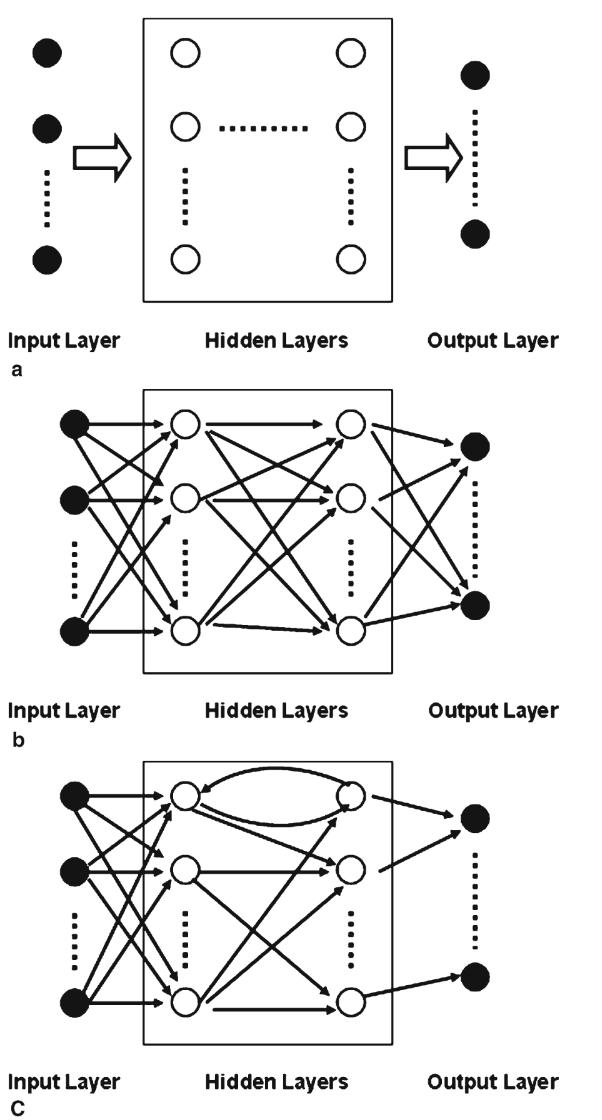
\includegraphics[scale=0.4]{NNTopology}
\end{center}
\caption{Topology sketches for neural networks. A) depicts the general topology, b) is a feedforwad ANN and c) a feedback ANN \cite{zou2009overview}.}
\end{figure}

\subparagraph{Learning} Learning describes the process of adjusting each weight of the inputs of each neuron. During the learning phase, these weights are adjusted until the output is equal or close to the target output. Furthermore, this process can be classified into \emph{supervised learning} and \emph{unsupervised learning} \cite{zou2009overview}. In unsupervised learning, the neural network is just defined via its node characteristics and network topology and then immediately applied to its use case \cite{james2023unsupervised}. The aim of this approach is that the network itself discovers patterns within its input data that might not be perceptible or thought of by humans \cite{james2023unsupervised}.
In contrast, supervised learning employs a dedicated learning and application phase. Within the learning phase, the network is given a training data set (which should be a representative model) where for each input the desired output is well-defined \cite{wang2020supervised}. This could be, for example, an audio file of someone talking (input) and its transcript (desired output). Using this training set, the neural network then adjusts its weights  so that it generates the same  or very similar output. 
Once the training phase is complete, the weights are fixed and the neural network can be applied where needed \cite{wang2020supervised}.  \\
While not relevant for the scope of this thesis, there exists yet another type of neural network learning. In \emph{reinforced} learning \cite{mahesh2020machine}, the network aims to maximize its performance in regard to a predefined dimension. It thus does not try to classify input like the previously mentioned methods do, but rather adapts so that the highest value is achieved. This type of learning can be often seen within the scope of neural networks for game optimization. Within this context, learning can be viewed as educating a child: for every correct decision or move the network makes, it gets rewarded with a numerical value. For example, if the network completes a lap within a racing game, a positive reward could be given. However, if the network acts in an unwanted way (i.e. crashing into another car), it gets penalized with a negative numerical value. When training long enough, such networks can even surpass the performance of top level players \cite{mahesh2020machine}.

\paragraph{Variations} While the above explanation serves as a rough overview for neural networks, there are different types of networks which bolster additional properties that have not been discussed yet. A short list with the most prominent variations is listed below.

\subparagraph{Deep neural network} A deep neural network (DNN) is a network that consists of at least three layers: an input layer, a hidden layer and an output layer. The addition of hidden layers allow the network to mimic non-linear functions (i.e. XOR) and compute more complex tasks \cite{borisov2022deep}.

\subparagraph{Convolutional neural network} When using neural networks for image detection, \emph{convolutional neural networks} seem to be the current gold standard \cite{li2021survey}. CNNs differ from standard neural networks in that they limit the number of inputs per node (instead of connecting each node with all nodes of the previous layer) and that multiple connections can share the same weight \cite{li2021survey}. These two factors alone can massively improve performance and simplify the network, but at the cost of expressability. For the task of image detection, this trade-off seems to be worth it. However, a CNN might need to employ an additional hidden layer solely for the purpose of accounting for different views of rotated objects within the image, thus slightly increasing its complexity again \cite{li2021survey}.

\subparagraph{Graph neural network} Most neural networks deal with inputs that are real continuous scalar values (i.e. values within $\mathbb{R}$), which includes positive, negative, rational and irrational values, although the latter has to be approximated due to memory limitations. GNNs instead have graphs as input, which are not part of $\mathbb{R}$ \cite{scarselli2008graph}. While each graph could be pre-processed and converted into a set of vectors, which is then input into a conventional neural network, this pre-processing step often comes with the cost of information loss \cite{scarselli2008graph}. In contrast, a graph neural network is able to process graphs directly, with the need of converting it into vectors being non existent or at the very least only necessary in later stages \cite{scarselli2008graph}.

\subparagraph{Spiking neural network} As previously mentioned, while ANNs are already capable of some impressive tasks, they do not even come close to their biological counterpart. For an ANN to have the same capabilities as the human brain, it has to have a number of nodes and synapses magnitudes higher than the brain, which massively increases both computation time and energy consumption \cite{yamazaki2022spiking}. \emph{Spiking neural networks}, or SNN, aim to somewhat narrow this gap by introducing another feature into ANNs that nature already uses: time. In a SNN, each fired signal does not only affect its target by its weight, but also by the time it was fired. Furthermore, also the chronological order of different inputs arriving at a node can now also carry information \cite{yamazaki2022spiking}. With the addition of a time component, complex processes can be expressed by using a significantly smaller network, thus positively impacting both energy consumption and performance.
\section{Voice Recognition}
The invention of artificial neural networks provided massive benefits for voice recognition software. Almost every solution nowadays uses some kind of neural network in the background. Furthermore, with the increase of computing power and more research, the type of neural network applied also changed drastically within the last years. While for a long time, neural networks that were designed after the \emph{Hidden-Markov model} or \emph{Gaussian-Mixture model} were considered the only viable approach for voice recognition, a new challenger decided to step up and compete for this title \cite{9133298}. Due to their added complexity, \emph{Deep Learning} networks boast higher capabilities and provide better results than their predecessors.
Regardless of the type of network chosen, a given audio recording must undergo two steps before being provided to the network for maximum accuracy:

\begin{itemize}
\item \textbf{Pre-Processing}: The pre-processing step aims to normalize the given audio to some degree. This includes issues like noise, suppression, silence removal and channel equalization \cite{9133298}. By applying these steps, the network is presented with a smaller variety of audio files, thus making it easier to interpret them.
\item \textbf{Feature Extraction}: Using feature extraction, the neural network gains additional knowledge of the presented audio, which it can then in turn use for better interpretation \cite{9133298}. While there exists no definitive categorization, auditory features are often divided into \emph{linguistic} and \emph{acoustic} features. Linguistic features describe the information in the words. This includes the detection of whole key-words or other semantic markers. Using such features, the semantic content of the whole audio can be better estimated since most of the time, real life conversations also have a logical semantic structure (i.e., if the word "bear" is detected as a key word, it is more likely that surrounding words are forest-related rather than belonging in the domain of higher mathematical terminology).
In contrast, \emph{acoustic features} aim to convey the network how a person hears. For example, most people's hearings ranges from 20Hz-20kHz and are less sensitive at lower frequencies. Also, the analysis and extraction of melody, accent or intonation when talking are relevant types of acoustic features  that, when extracted, could potentially aid the neural network.
\end{itemize}

After these steps, the audio can be provided to the neural network. The network itself has usually been trained using a \emph{supervised learning} approach, i.e., a labeled data set (audio and transcripts) is provided in a learning phase. Once the learning phase is over, the weights for each node are fixed and the network is ready for productive use.

Since almost all Serious Games for speech rehabilitation use some kind of voice recognition or analyzation software, quickly introducing three variations is an effort well spent. The next paragraphs will shortly elaborate on three voice recognition systems: \emph{WhisperAI}, which is also used within Logopedic's Escape, \emph{VoiceItt} and \emph{Dragon NaturallySpeaking}.
\subsection{WhisperAI}
WhisperAI is a speech-to-text software developed by OpenAI. It applies neural network capabilities and also implements a novel \emph{Large-Scale Weak Supervision} approach \cite{radford2023robust}: The issue almost all neural networks face is the absence of high-quality training data. In the case of voice recognition, a dataset of around 1000 hours of supervised and labeled audio files is considered to be quite formidable. However, this number pales in comparison with the amount of data that could be used if manual labelling would not be an issue.
Thus, to both increase data quantity and keep quality relatively high, WhisperAI uses a so-called \emph{Weak Supervision dataset}. This dataset consists of 680 000 hours of multilingual audio files which were previously labelled not by hand but automatically using another voice recognition software. This approach has led to create a robust and well-generalized neural network that even supports multiple languages.
\paragraph{Network architecture}
While OpenAI offers access to the full WhisperAI instance via API-calls, they also provide smaller images that can be used locally:
\begin{table}[h]
\begin{center}
\begin{tabular}{|c|c|c|c|}
\hline
 \textbf{Model} &  \textbf{Layers} & \textbf{Nodes/Layer} & \textbf{Size (Mb)} \\ \hline 
\textbf{Tiny} & 4 & 384 & 39 \\ \hline 
\textbf{Base} & 6 & 512 & 74 \\ \hline 
\textbf{Small} & 12 & 768 & 244 \\ \hline 
\textbf{Medium} & 24 & 1024 & 769 \\ \hline 
\textbf{Large} & 32 & 1280 & 1550 \\ \hline 

\end{tabular}
\caption[WhisperAI Models]{Local image specifications of Whisper models.}
\end{center}
\end{table}

\paragraph{Training}
For training, the data first had to be pre-processed and normalized. All audio files were thus re-sampled to 16kHz and a volume normalization between -1 and 1 was done. Then, the model was trained for $2^{20}$ updates, each containing 256 audio segments from the data set. This process culminates in every segment within the dataset being used two to three times within the training process.

\paragraph{Results} 
The capabilities of a voice recognition software is often measured using the \emph{Character error rate} (CER) or \emph{Word error rate} (WER). CER is defined as the relative amount of characters that were wrongly transcribed compared to all characters. For example, if 1 out of 10 characters is transcribed incorrectly, the CER would be 10\%. The WER is an extension of CER applied to whole words. Naturally, WER therefore has to be always higher than CER.
When testing WhisperAI using the "Large" model on common datasets, the WER was comparable to that of professional human transcribers, with Whisper slightly underperforming by a fraction of a percentage \cite{radford2023robust}.
\subsection{VoiceItt}
VoiceItt is another speech-to-text software that is specifically tailored to aid people with speech impediments \cite{howarth2024developing}. Like WhisperAI, it also uses artificial intelligence to learn a generalized speech pattern. However, patients who want to use VoiceItt have to additionally read in 200 voice cues themselves in order for the recognition to work optimally. While this approach of customization is beneficial for all recognition systems, it is that much more important for speech impeded users as each impediment can stem from another source, therefore allowing for much higher speech variation. Sadly, the author could not find any more details regarding architecture details and learning process. Presumably, VoiceItt omits this data on purpose in order to keep their competitive advantage.

\paragraph{Results}
Again, there is no scientific evidence that support using VoiceItt has more of a positive impact on speech impeded users than traditional voice recognition systems. However, there has been a field study \cite{howarth2024developing} with over 60 participants from the UK and Ireland that used the VoiceItt App and reported their experience. In this context, the consensus was that VoiceItt performs better compared to other recognition softwares, but could not be considered groundbreaking.

\subsection{Dragon NaturallySpeaking}
Within the field of dictating, Dragon by Nuance has been a long-time competitor with its first version release all the way back in 1997 \cite{mccrocklin2020revisiting}. Within recent years, Nuance also implemented a neural network approach within their products. Furthermore, they offer specific versions depending on their intended usage environment. For example, \emph{Dragon Legal} has been trained specifically for court usage, meaning it can better understand law-related terms. On the other hand,  \emph{Dragon Medical One} would be the preferable choice within the health sector. However, while the Dragon products are considered to be some of the most frequent and matured recognition technologies used \cite{shadiev2023review}, they do come at a hefty price tag of, depending on the specific product, upwards of \$500 \cite{Nuance}. Since Dragon is also a commercial product like VoiceItt, the author could also not find any details on the concrete learning process or architecture used.

\paragraph{Results}
Although Dragon seems,  to stand in high regards within the field of dictation, no scientific evidence regarding its precision or other performance factors could be found. However, disregarding its high price tag, studies that research on voice recognition software tools and their usability seem to hold it in high regard \cite{shadiev2023review, gandara2016voice}.


\section{User Centered Design}
User Centered Design (UCD) describes a methodology for developing products with a high involvement of at least one of its destined user groups. Often, the experts developing a product fail to view it through the eyes of its typical user, which leads to an undesired output. To counter this issue, UCD actively includes the end user of the product via questionnaires, interviews or testing phases \cite{9255313}. The rough process of UCD looks as follows, although specific implementation might differ \cite{7881322}:
\begin{itemize}
\item \textbf{Step 1: Field Study} By conducting interviews and observing the users in their environment, an initial understanding of the work- and information flow can be acquired. Additionally, this phase is often used to convince users to join the UCD-process. Within this phase, no actual development occurs and possible participants are not yet actively contributing. This phase is meant to provide developers with both domain and process knowledge needed in further steps.
\item \textbf{Step 2: User Workshops} Previously identified participants are invited to join a user workshop in order to better define the user's requirements regarding the product. These workshops have to leave room for active participation by limiting the amount of frontal lecturing and incorporating activity-promoting measurements (i.e. provide pen and paper for rough prototyping). In this phase, developers and participants aim to conjointly create and discuss ideas and requirements. While participants are most likely to describe desirable requirements, it is the developer's task to verify whether those requirements are feasible and, if necessary, inform if additional resources might be necessary. Depending on the group size, open-questioned one-on-one interviews might also be applicable.

\item \textbf{Step 3: Design and Development} The previously deducted user requirements are being implemented within the product. During this phase, participants still work with an older version of the product while the developers actively implement previously discussed requirements.

\item \textbf{Step 4: User Evaluation} A prototype of the product is presented to the users, which in turn are encouraged to test it out. The testing process can be structured rather simple (i.e., letting the user test the product and note down their feedback regarding usability or functionality) or more complex (i.e., using standardized laboratory test environments, using questionnaires, ...), depending on group size and fund availability. Furthermore, the testing pool size can also be adapted. Ideally, the prototype is tested by multiple users in order to get more diverse feedback. However, if the testing pool becomes too large, additional costs and time must be allocated. Additionally, if for example a whole department were to test this prototype, it is also possible that single users might continue using this prototype for productive work even though flaws still persist. If any flaws or missing features are detected within this step, the product will be adapted accordingly (Step 3) before being evaluated again (Step 4). The next step will only be executed once the users are satisfied with the product.

\item \textbf{Step 5: Field Trial} Once all initial issues have been addressed, it is recommended to conduct an active field trial to observe the product's long-term usage. This step is crucial since not all issues might be detected within the previous step. However, in practice this step is often skimmed or skipped entirely due to budgeting reasons.

\item \textbf{Step 6: Final Deployment} If the field trial yields acceptable results, the product can finally be deployed. At this point, the project can be regarded as complete. If the need to change the product arises in the future, a new UCD-cycle can be started.
\end{itemize}

In addition to the rough process structure mentioned above, the core principle of UCD also adheres to fundamental guidelines regarding the development process. Still et al. \cite{still2017fundamentals} describes these guidelines as \emph{The 10 UCD Commandments}, and although this list is likely to not be exhaustive, regarding these commandments is recommended for the UCD process:
\begin{enumerate}
\item \textbf{Involve users early} Best results are achieved by incorporating end users as early as possible into the process. A common belief is that users should only be involved once a usable artifact, such as a prototype, has been implemented, but user recruitment can start event prior \cite{still2017fundamentals}.
\item \textbf{Involve users often} If users are consulted more frequent, it is more likely that developers are more aware of the user's current experience and needs and therefore are able to quickly act accordingly \cite{garrett2022elements}.
\item \textbf{Design for use in context} When developing a product,  it is important to consider the environment in which the product will be used. Ideally, the product design accommodates for this accordingly \cite{still2017fundamentals}.
\item \textbf{Keep it simple} If the product is too complicated, users are likely to become frustrated when using it. Therefore, simplifying the product, if possible, is recommended \cite{colborne2017simple}.
\item \textbf{Be polite} Users will always attempt to use the product in the most simple way possible. Thus, the product has to be designed as simple as possible in order to be polite to the user and to not convey incompetence \cite{cooper199914}.
\item \textbf{Know your users} Developers have to know their users' wants and needs in order to develop a suitable products. Therefore, this commandment states that developers should directly interact with the users in order to better understand them \cite{still2017fundamentals}.
\item \textbf{Give users control} The product must allow the user to have as much control over it as possible. This means that the product should allow the user to manually start and stop most processes as well as provide better situation awareness \cite{jones2004designer}.

\item \textbf{Remember to design for emotion} In the end, users are also just humans and, as such, feel just as much as they think. Therefore, providing a visually pleasing appeal results in higher satisfaction and acceptance \cite{still2017fundamentals}.
\item \textbf{Trust, but verify} Developers are encouraged to trust in their instincts and what they learned by talking to users. However, this trust has to be verified frequently via testing phases or collecting feedback \cite{morgan2004360}.
\item \textbf{Discover before designing and delivering} Before developing the product, it is highly beneficial to first regard both the application environment as well as user's wants and needs as much as possible. Multiple feedback rounds before and during the design process are just one tool for this. However, one must also be aware that most likely new issues or requirement ideas will arise even after the product has been delivered \cite{still2017fundamentals}.
\end{enumerate}
%\paragraph{UCD in Healtcare}

\section{Summary} This chapter provided some insight regarding the theoretical background which this thesis' practical part builds up upon. \\
Serious Games are a subcategory of games which aim to provide some additional kind of benefit besides entertainment to its user (i.e., education or healthcare). Within Serious Games, the class of healthcare games are games which focus on improving the well-being of their users and can again be further categorized regarding their intended benefit and usage. Some examples of this are exergames, distraction games and recovery and rehabilitation. Furthermore, Serious Games are also used for training medical professionals. This can reach from surgery simulations or mobile anatomy atlases to simulated patient cases for which the correct diagnosis and treatment has to be found.
\\
Regarding speech impediments, there exist two different main categories: apraxia and aphasia. Depending on the severity and progression, patients might even suffer from PPAOS, which describes a form of apraxia that worsens if left untreated. Similarly, aphasia can also be further categorized into svPPA, non-fluent PPA, logopenic variant PPA or PPA mixed, depending on the type of symptoms. While apraxia is a speech impediment which stems from the loss of facial and laryngeal muscle control, resulting in slurred speech, aphasic patients are unable to understand the meaning behind words, therefore they might talk fluently but do not know what the words spoken mean. Both impediments are most often caused by a previous brain injury, whereas strokes are the most prevalent.  If left untreated, more severe forms of apraxia and aphasia can manifest over time, leading to higher dependability. Regarding therapy, both apraxia and aphasia benefit from regular speech training which include as many other senses as possible. Additionally, aphasic patients might fare better by adapting a new custom alphabet or ingesting pharmaceutics, though their effectivity is still somewhat unclear. Last but not least, both apraxia and aphasia are most commonly results of brain impairment. It is most often stroke patients that suffer from those impairments, although both age and gender are suspected to be comparably marginal risk factors as well.
\\
However, as practice has shown, therapies and rehabilitation measurements prescribed to patients can only aid if they are followed. While almost every patients wants to improve upon their health, not all seem to follow medical advice as they are supposed to. This is known as compliance or therapeutic compliance within healthcare. Depending on the type and duration therapy, the rate of compliant patients is as low as 20\%-30\%. The reasons for non-compliance seem to be many in numbers, but can be roughly classified into patient-related, therapy-related, social and economic factors. Out of these categories, therapy related reasons seem to be the most impactful, meaning patients do not enjoy their treatment plan as much as they should. This is a known issue and one possibility to mitigate this issue is to provide multiple treatment methods within therapy, one of which could be the application of Serious Games.
\\
A neural network is a machine learning technique used for classification or optimization problems. Like its biological counterpart, an artificial neural network consists of neurons (nodes) and synapses (links between nodes). Depending on the input of a node, a node might or might not fire a signal to its outgoing synapses, which in turn can excite other neurons. The activation of a node depends on a summary of features called node characteristics. Those describe the structure of the node, including the number of inputs and their weights, number of outputs and the activation function. The activation function describes which sum of inputs creates which output. This can be either a simple binary step function, in which the output of the neuron is either 0 or 1, or something more sophisticated like the identity or tanh function. As of now, the most common type of activation function is the ReLu functions and its variants due to is high expressability and advantageous performance. Neural networks are usually divided into layers of neurons. Depending on whether the network is regarded as feedforward or feedback network, different rules regarding output direction for each node apply. When training a neural network, one can either implement a supervised (i.e. includes a training set for which the desired output is already known) or unsupervised (i.e. a training set without known output) approach, both bearing their own advantages and drawbacks. Last but not least, some common variations of neural networks include DNNs, CNNs, GNNs and SNNs, each of them providing different advantages depending on their usage. \\

Regarding voice recognition, the usage of neural networks has become state of the art. To achieve the best results, however, any audio recording has to be somewhat normalized using a pre-processing step, as well as have certain features or information highlighted. Both steps provide stability and additional information to the network, increasing recognition rate. \\

Last but not least, the user centered design (UCD) methodology was quickly explained. The main gist of this approach is to actively incorporate users within the development process of the product. This  ensures that the final product fulfills the wants and needs of the user better when compared to traditional development. The UCD process can be divided into different stages, starting with a general field study and ending in a field trial and deployment phase. Note that not all UCD-projects strictly follow these steps as there is no single definition of UCD, as it rather describes a paradigm or scheme.


\chapter{State of the Art}
\label{chap:state}
This chapter will elaborate on the current State of the Art for both speech rehabilitation games and voice recognition software. After extensive research, a total of six Serious Games were chosen for further elaboration: Treasure Hunters \cite{TreasureHunters}, Training with Phonak \cite{Phonak}, Opera Singer \cite{ParkinsonGame}, Apraxia World \cite{hair2021longitudinal}, Flying Rocket \cite{takagi2020voice} and Talking to Teo \cite{navarro2014talking}. Those games were chosen specifically either due to their popularity (i.e., Apraxia World), novelty (i.e., Flying Rocket) or size and quality of field tests (i.e., Treasure Hunters) if available. For each of the game, a short game description and, if available, public results of a field study including the game are presented. However, as previously mentioned, none of those games bolster themselves with providing an adequate voice recognition component. Thus, after elaborating and comparing these games, voice recognition softwares are introduced next and compared as well. For the purpose of this thesis, a total of three softwares were examined: WhisperAI \cite{radford2023robust}, VoiceItt \cite{howarth2024developing}, and Dragon NaturallySpeaking \cite{mccrocklin2020revisiting} .
\section{Speech Rehabilitation Games}
There have already been various Serious Games developed for speech impeded patients which are worth introducing and analyzing them regarding their capabilities.
\subsection{Treasure Hunters}
Treasure Hunters was created by Mario Ganzeboom, Marjoke Bakker and Toni Rietveld at Radboud University Nijmeng in the Netherlands \cite{TreasureHunters}. It primarily targets patients that suffer from \emph{dysarthria}. Patients who have this condition have limited articulation capabilities and struggle regulating their speech volume, making them difficult to understand. Furthermore, the authors of this study realized that currently verbal human-computer-interactions and their application within training and rehabilitation settings are far from optimal. While such applications do provide a benefit via their drill-and-practice approach, patients reported that exercising in this fashion feels "off" and that the gap between such training sessions is "far from daily functional communication" \cite{TreasureHunters}. As a result, the decision was made to design the game to support inter-human communication as to better mimic day-to-day verbal interactions.

\paragraph{Game Description} Treasure Hunters is an online two-player game. Each person controls one of two characters: the \emph{diver} or the \emph{digger}. The goal for both of them is to find and open a treasure chest buried deep beneath. In order to succeed, they need to retrieve two items: the treasure chest and its key. The digger tries to acquire the chest while the diver searches for the key. However, they cannot succeed in this task alone because they do not know the exact location of their sought item. It is the other player who holds this information (i.e., the digger knows where the key is and the diver knows where the chest is), therefore both players have to communicate with each other to share the location details, practicing their speech capabilities together.
The communication occurs online so that both players can play in their homes. Additionally, the transmitted communication gets analyzed based on the \emph{Pitch Limiting Voice Treatment} (PLVT) \cite{de2003improvement} standard. This standard determines which volume and pitch is adequate for communication. If a player speaks too high-pitched or quietly, they will be informed of it and can adapt accordingly. The desired range for volume and pitch was set to 60 decibels or above and 170 Hz or below for every player.

\paragraph{Results} To measure whether Treasure Hunters provides any additional benefit compared to classical therapy, a total of seven participants which either suffered from Parkinson's Disease or a stroke were included within a field study. All participants received at least 6 months of classical speech training beforehand. Due to medical reasons, two participants had to prematurely quit the study, but the remaining five separated into two groups. One group would exercise with classical therapy while the other one played the game for four weeks. Within these four weeks, the participants exercised four times per week for 15 minutes with the game or within therapy. Afterward, individual progress was evaluated. Then after a two-week resting period, participants were evaluated again to measure the longevity of the progress made and then the groups switched activities for another four weeks. In the end, each participant thus had four weeks of playing the game and four weeks of classical therapy within the study. To test for changes in intelligibility, the participants had to undergo four measurements, one before and after each four week practicing period. Within each measurement, participants had to read a short 30 sentence story out aloud, which was identical for all measurements. When the experiment ended, university students were then asked to rate each measurement pair (i.e., the recordings of a participant immediately before and after a  four-week training block) on a scale from -3 (the recording before the training block is much better) to 3 (the recording after the training block is much better). 
\\ As a result, the study concluded that there was no clear benefit of playing Treasure Hunters regarding therapy progress when comparing it to the traditional approach. However, not every patient is equal, and it is fair to assume that some would prefer to play a Serious Game within therapy context. Thus, the final verdict of the study is that Serious Games can only be applied on an individual basis.
\begin{figure}
\begin{center}
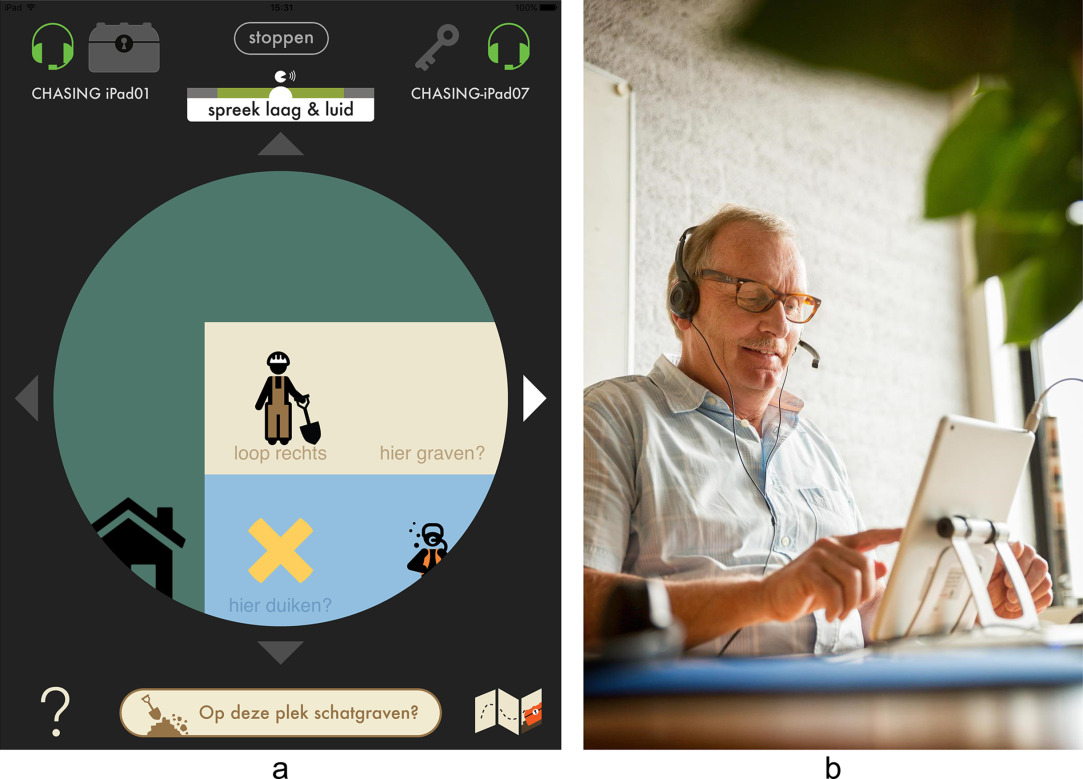
\includegraphics[scale=0.4]{TH_Game}
\end{center}
\caption{Screenshot of Treasure Hunters\cite{TreasureHunters}.}
\end{figure}
\subsection{Training with Phonak}
Training with Phonak was developed by researches of the IDIS department of the university of San Buenaventura in Colombia in 2015 \cite{Phonak}. Its main audience are children that suffer from hearing deficits or loss and, as a result, have received an artificial cochlear. Any patient that has received such a cochlear is expected to participate in \emph{auditory-verbal therapy (AVT)} to regain their hearing. AVT describes an extensive therapy process that, while effective, can be quite monotonous and boring, especially for children. AVT consists of  30-minute therapy sessions once per week and incorporates many materials like pictograms, papers, and toys. Since so much different material is needed, most often therapists work with a limited material set, making the therapy repetitive and boring. Furthermore, each session has to be evaluated and tracked by the therapist, which takes up additional time. Training with Phonak was therefore developed to counteract these issues. It was created with the help of twelve children between 7 and 11 years in order to evaluate which aspects would make the game fun and easy to play. One of those requirements was that the game should be available for smartphones or tablets, as not every child has access to a PC. Additionally, the game must be diverse and introduce new gameplay mechanics frequently in order to not become stale. The game consists of five stages which tightly correlate with the five steps of rehabilitation: Detection, discrimination, identification, recognition, and comprehension.

\paragraph{Game Description}
The main character of the Game is called Phonak. Phonak got lost on an unknown planet called Sounds. For him to return to his friends and family, Phonak has to travel to multiple planets and overcome tough situations. In the process, Phonak acquires new abilities that support him on his journey. These skills are key elements of the five steps mentioned above. For every activity the player performs, the game gathers logging information which the therapist can inspect afterward.

\paragraph{Results}
There is no published documentation regarding the methodology or results on the effectivity of Training with Phonak. It is known, however, that the game used a \emph{user-centered-design (UCD)} approach during development, meaning that during implementation, patients have given continuous feedback in order to further improve the game.

\begin{figure}
\begin{center}
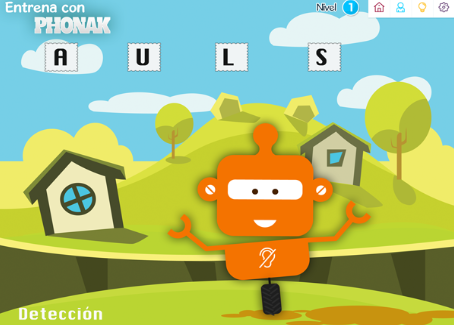
\includegraphics[scale=0.5]{Phonak_Game}
\end{center}
\caption{Screenshot of Training with Phonak\cite{Phonak}.}
\end{figure}
\subsection{Opera Singer}
Opera Singer was developed by researchers of the university of Hannover and Bremen in Germany \cite{ParkinsonGame}. It is a single-player game which aims to aid patients suffering from dysarthria resulting from Parkinson's Disease, which is the same target audience as the previous game Treasure Hunters. Note that "Opera Singer" is not the official name of the game, but since the original creators did not name their game, the game will be called "Opera Singer" within this thesis for the sake of simplicity.

\paragraph{Game Description} 
While \emph{Opera Singer} is not the official name of the game, it certainly describes the main gameplay quite well. In the game, the patient acts as an opera singer who tries to shatter a glass with only their voice. To achieve this, the player has to maintain a certain speech volume for a defined time. The intensity and duration of this action depends on the type of glass (i.e., a porcelain vase, a beer jug, a milk glass or a martini glass) that has to be shattered. Depending on the difficulty of the glass, the player gets awarded more or fewer points upon shattering it. The game can be played indefinitely, as any broken glass is simply replaced.

\paragraph{Results}
In order to verify the game's effectivity, it was evaluated by eight participants (four male and four female) with varying stages of Parkinson's Disease. The mean age of these participants was 70.75 years, with the oldest and youngest being 79 and 56 respectively. Furthermore, seven of the eight participants have never received voice therapy beforehand.
Before playing the game, each participant had to shortly warm up in order to increase respiratory activity and therefore  vocal performance. Additionally, each patient had to do a voice self-assessment test and their maximum volume intensity was noted in order to establish a ground truth. Then the patients had to play the game until they at least reached a score of 300, upon which their maximum volume intensity would be evaluated again.
The results speak for themselves; at the second intensity test, each patient managed to increase their volume intensity by at least 4.93 dB and up to 20.09 dB. Last but not least, seven out of the eight patients said they enjoyed playing the game and would consider doing it again.
\begin{figure}
\begin{center}
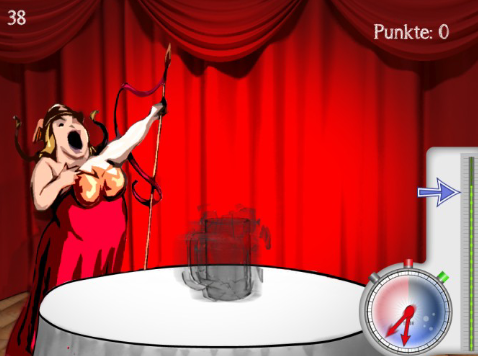
\includegraphics[scale=0.5]{OperaSinger_Game}
\end{center}
\caption{Screenshot of Opera Singer\cite{ParkinsonGame}.}
\end{figure}
\subsection{Apraxia World}
Apraxia World is a 2D platformer game developed by researchers from both Australia and the USA. Its target audience are children suffering from speech impediments. The game was developed using the Unity Engine and is based on an existing game called \emph{Ekume Engine 2D} but expands on it by incorporating voice therapy elements \cite{hair2021longitudinal}.

\paragraph{Game Description}
In Apraxia World, the player controls a monkey whose goal it is to reach the end of the level. To accomplish this, the monkey has to run and jump from platform to platform while avoiding holes and enemies. On their way to the finish line, the player can also collect stars which are necessary to unlock further levels along the way. To collect these stars, the player has to first reach them and, upon touching it, solve a speech exercise. These exercises mostly consist of saying a word clear enough so that the game can understand it. Doing so correctly or failing five times collects the star.
Additionally, the monkey only possesses a limited energy supply. Once depleted, it becomes slow and its jumping height decreases dramatically, making the game much more difficult. However, the player can replenish the monkey's energy by again solving short speech exercises. For each word spoken correctly, the monkey gains 10 more seconds worth of energy and for every incorrect attempt it gets 5.
As of now, the game consists of five different worlds with eight levels each, as well as a customization shop where player can buy accessories for their character in exchange for coins collected within the levels. Furthermore, players can also buy temporary power-ups in the shop, including a shield against enemy attacks, the ability to fly, a coin magnet or a score multiplier.

\paragraph{Results} 
The game was evaluated using 11 children between five and 12 years of age, although one child had to withdraw from the study due to schedule conflicts. For each child, a separate list of words which the child practices within the game was acquired and integrated into the game. Thus, the game was personalized for each child's specific needs. Then the evaluation phase went as follows: 
\begin{itemize}
\item \textbf{Week 1}: Setup/Calibration for each child's needs. This includes the word lists as well as an initial voice test.
\item \textbf{Week 2-5}: First treatment phase. In this phase, the children played the game for four days per week. At the end of each week, they underwent a small test to measure their progress. Additionally, the voice feedback system used was either automated or simulated by a wizard-of-oz setup (i.e., caregivers would give feedback to the child's input in a hidden manner). To measure engagement, the children filled out two questionnaires regarding their subjective experience with the game in this time period. Furthermore, the game also logged player activity (i.e., successful and failed pronunciation attempts) and saved all recordings for later analysis.
\item \textbf{Week 6-7}: Break phase. Here the children did not have to play the game. At the end of the second week, another voice test was conducted to determine whether previous improvements were still present.
\item \textbf{Week 8-11}: Second treatment phase. This phase was identical to the first one, with the small difference that children who previously got feedback via the automated voice feedback system would now get it by their caregivers and vice versa.

 
\end{itemize} 
After these 11 weeks the results were analyzed regarding gameplay, therapeutic progress, audio quality and pronunciation evaluation. Regarding gameplay, metrics like playing time, game progression and in-game purchases over the course of the experiment's duration were taken into consideration. To measure therapeutic progress, the initial baseline test done in week 1 was compared to a final test after week 11. Also, in-game logging data regarding correct or faulty pronunciation was examined in order to detect performance trends.
To quickly summarize, the game succeeded in capturing the children's attention over a long time and the therapy progress measured was similar to regular therapy.
\begin{figure}
\begin{center}
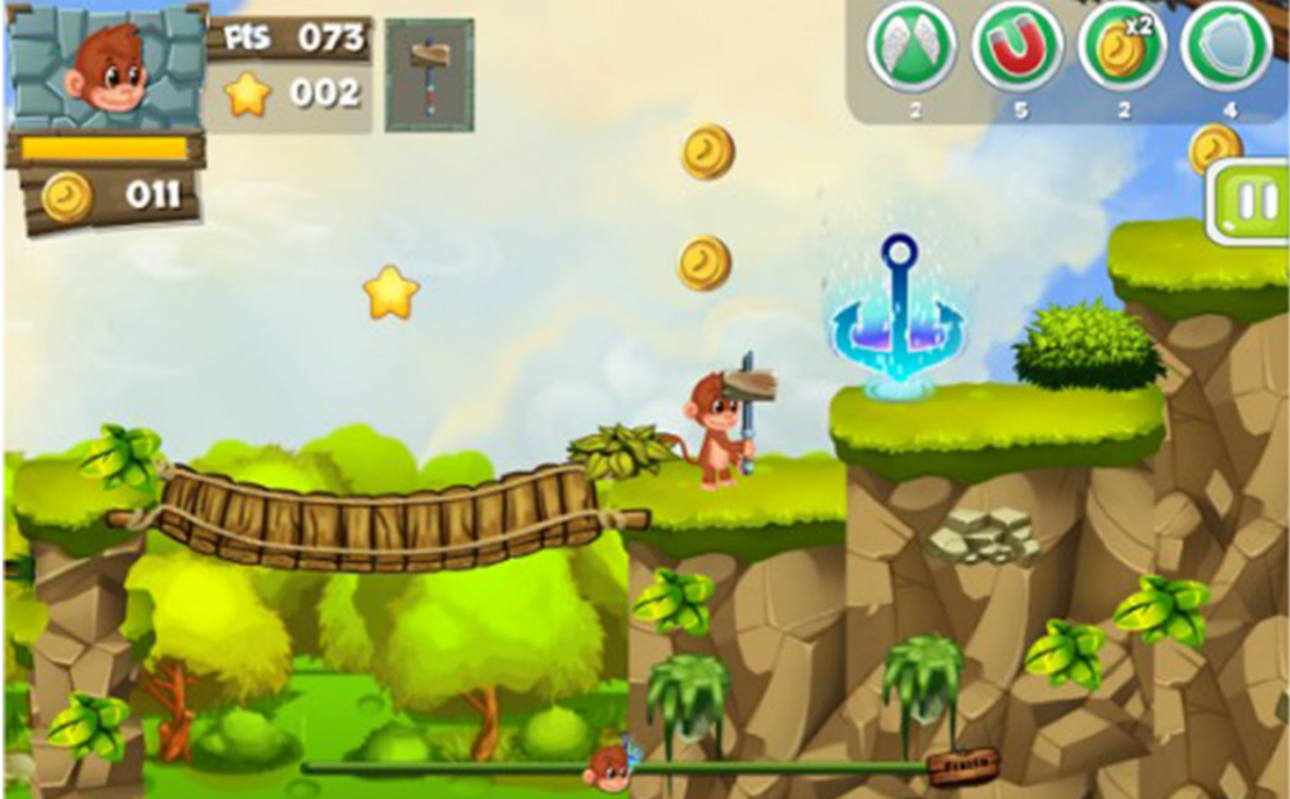
\includegraphics[scale=0.25]{Apraxia_Game}
\end{center}
\caption{Screenshot of Apraxia World\cite{hair2021longitudinal}.}
\end{figure}

\subsection{Flying Rocket}
Flying rocket is another 2D game developed using the Unity Engine. The project was created by a collaboration of members of Meisei University, Tokyo University of Technology and Ochanomizu University, all of which are located in Japan. Again, this game targets young children suffering from hearing disorders. What makes the game stand out from the other ones previously described is that it uses both vocal and visual input (i.e., mouth gestures) to determine the correctness of spoken words \cite{takagi2020voice}. 

\paragraph{Game Description} 
The game itself is rather simple. The player controls a rocket ship which is trying to fly to the moon. To do so, the player has to correctly pronounce the given word. Depending on the accuracy of the pronunciation, the rocket will either fly towards the moon or lose height and return towards earth. If the pronunciation accuracy reaches a predefined threshold, the rocket safely lands on the moon.

\paragraph{Results} As of now, the game has yet to be evaluated by real patients. It is furthermore unclear whether the authors of the game intend on doing so in the foreseeable future.

\begin{figure}
\begin{center}
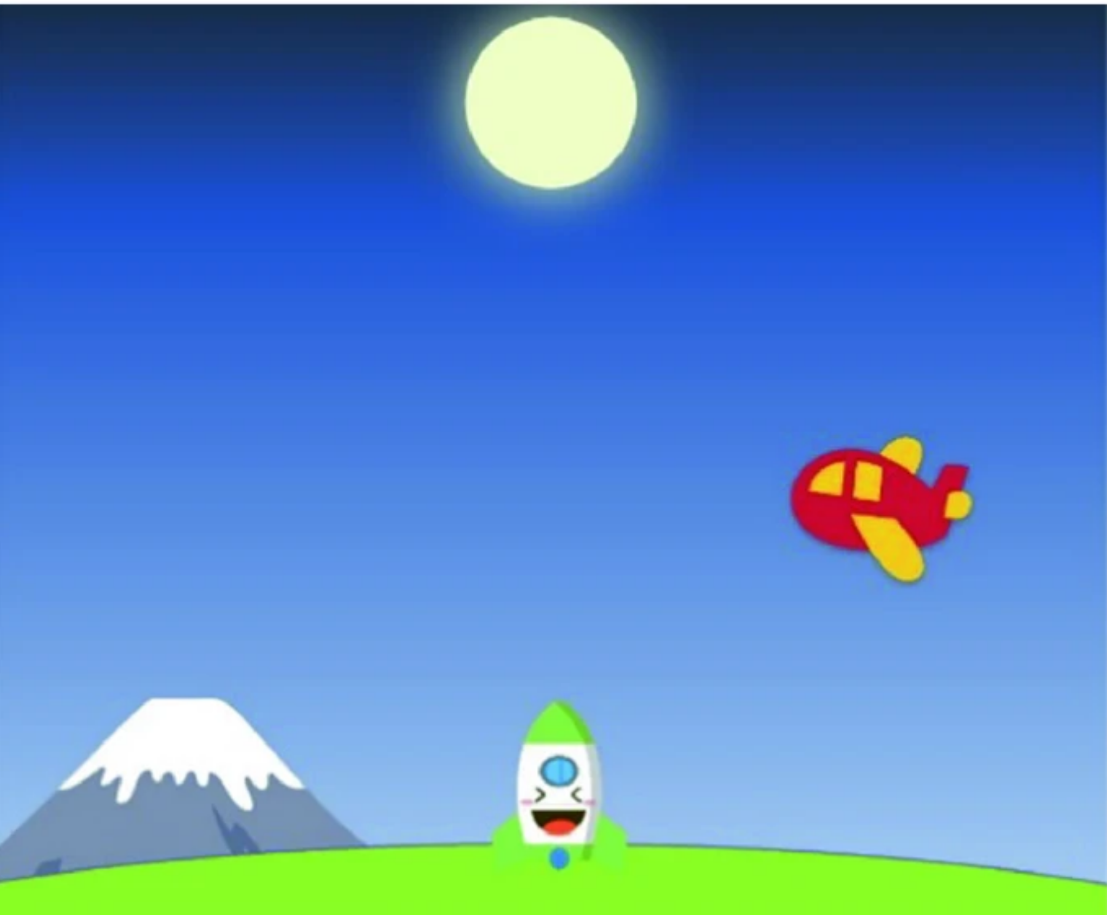
\includegraphics[scale=0.25]{Rocket_Game}
\end{center}
\caption{Screenshot of Flying Rocket\cite{takagi2020voice}.}
\end{figure}


\subsection{Talking to Teo}
Talking to Teo is a 2D game aimed for young children (3-11 years old) which have previously received a cochlear implant and thus have to undergo additional speech therapy. It was developed by researchers of Colombia and, unlike all previously mentioned games, is completely in Spanish. What further makes the game stand out is that it heavily includes the therapist within the process: for the game to be played, a "recipe" has to be first issued. The recipe states which and how often certain sounds have to be exercised within the game. It can be created using the game's web interface, which provides an overview of all patient data regarding the game for the therapist. When the recipe has been created it is then fed into the game and executed within its context, meaning levels are tailored to fit the recipe, and logging data will be collected accordingly. After playing, the therapist can then view the player's performance on the web interface \cite{navarro2014talking}. 

\paragraph{Game Description}
The game tells a story about a bear called Teo. Teo lives alone in a wildlife zoo but wants to find friends since he heard that evil hunters are nearby. While searching for other bears, he encounters a squirrel that wants to aid him on his journey. In order to both explore new areas of the zoo and find clues about the other bear's whereabouts, Teo has to complete different minigames provided by the squirrel (i.e. filling a bucket with honey or opening treasure chests by voice). To do so, the player has to complete the above mentioned recipes correctly. Each minigames must be repeated for at least ten times, whereas eight times it has to be successfully completed. If this is the case, the player is rewarded with another piece of the zoo's map, unlocking new minigames and new stages. As of now, the game consists of two distinct story stages with no definitive ending as the second stage can be played indefinitely.

\paragraph{Results}
The game was tested by fifteen children between the age of four and twelve. The consensus was that the game was fun to play and motivated the children to do more. Only the usability took a small hit within this evaluation.
Regarding the therapist, she was highly interested in the game and expressed its usefulness within the therapy scope. Some small adjustments like naming conventions and the likes had to be made after testing, but overall, the game was received quite well.
\begin{figure}
\begin{center}
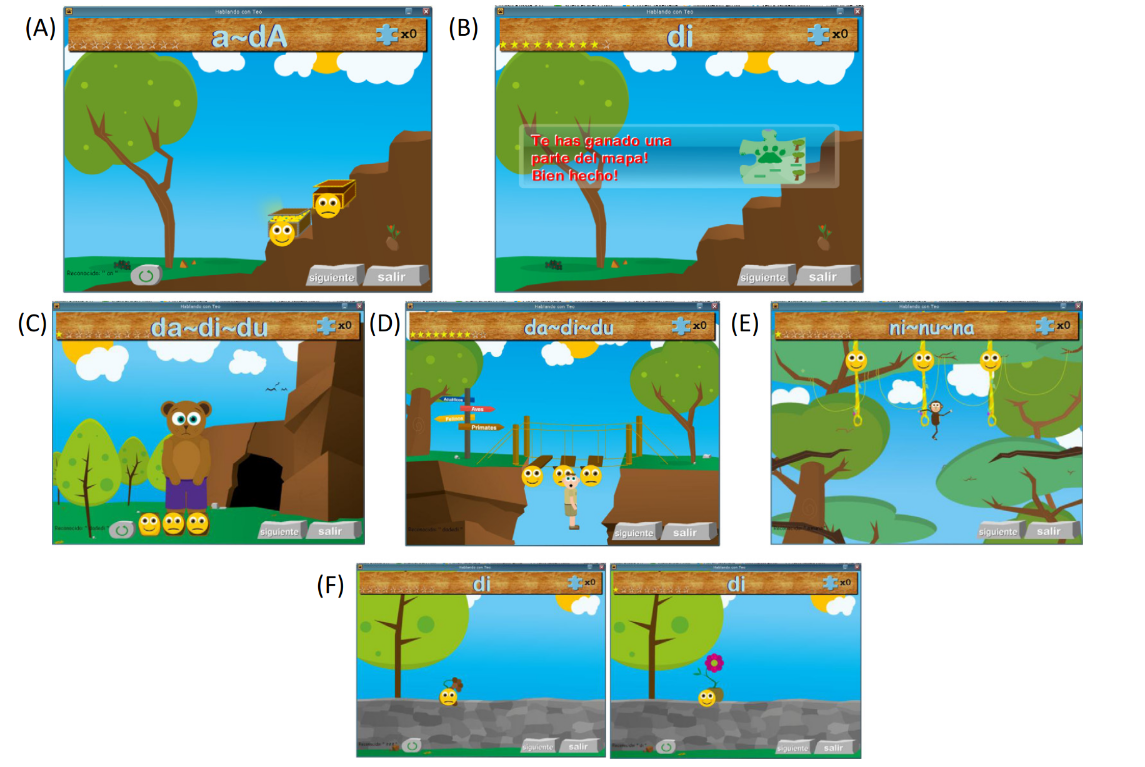
\includegraphics[scale=0.4]{TTeo}
\end{center}
\caption{Screenshot of multiple minigames of \emph{Talking to Teo}\cite{navarro2014talking}.}
\end{figure}

\subsection{This work}
The game which was developed within the context of this thesis is a direct continuation of a previously developed version implemented by the same authors \cite{LEPaper}. This first version was meant to be a proof-of-concept prototype which,  while playable, was still missing many important requirements. More specifically, the game included a hardcoded first level for which multiple components (i.e., the speech recognition module or various helper-features) were mocked, meaning their functionality was not fully realized. To put this previous work into context, this version of the game roughly covered the first phase of this thesis' course of action as described in chapter \ref{chap:coa}. \\
Thus, it should also be noted that all of the requirements listed in \cite{LEPaper} are also present in this thesis (see Table \ref{tbl:requirements}). Notable additions that were made within this thesis were, however: 
\begin{itemize}
\item The addition of a level editing feature.
\item The introduction of categories (i.e., grouping of multiple levels for a specific therapy use-case)
\item Implementation of various assistance features.
\item Implementation of a custom voice recognition model tailored specifically for speech rehabilitation usage.
\item Addition of logging capabilities and progression metrics
\item Implementation of a "child mode", i.e., a game mode specifically made for children
\end{itemize}
These are just some added features, for a full listing please refer to Table \ref{tbl:requirements}. \\
As a result, the Serious Game developed within this thesis' scope boast multiple advantages when compared with current solutions. For example, by letting the therapist create custom levels specifically targeted to the patient (a functionality none of the previously introduced Serious Games possess to this extent), a more individualized experience can be created, thus further aiding therapy progress. Additionally, no other Serious Game covers all three voice therapy stages (i.e., phonetic, syllabic and words), the best any other game has accomplished were two stages. By covering all three stages, the Serious Game becomes more versatile in its application and can be used for a prolonged period of therapy time. Last but not least, this Serious Game also employs a voice recognition component using artificial intelligence which has been specifically trained for voice therapy usage, a feat that has yet to be replicated.

\paragraph{Previous results}
Since the game was still lacking critical features at this point, it was not considered suitable for distribution to patients or other volunteers for evaluation purposes. Thus, no information regarding the game's reception and therapeutic impact could be collected. However, the therapist who aided in the development process stated that the game had potential and, if developed further, could prove to be useful for therapy.
\subsection{Summary}
Table 3.1 summarizes all presented games, including the author's own one regarding their capabilities.
\begin{sidewaystable}[h]
\begin{center}
\begin{tabular}{|c|c|c|c|c|c|c|c|c|c|}
\hline
&  \scriptsize{\textbf{\makecell{Single-\\player}}} &  \scriptsize{\textbf{\makecell{Voice \\analysis}}} & \scriptsize{\textbf{\makecell{Voice \\ Recognition}}} & \scriptsize{\textbf{\makecell{Progressive \\ difficulty}}} & \scriptsize{\textbf{Phonetic}} & \scriptsize{\textbf{Syllabic}} & \scriptsize{\textbf{Word}} & \scriptsize{\textbf{\makecell{Lip\\ images}}} & \scriptsize{\textbf{3D}} \\ \hline 
\textbf{\makecell{Treasure \\  Hunters}} & $\times$ & \checkmark & $\times$ & $\times$ & $\times$ & $\times$ & \checkmark & $\times$ & $\times$ \\ \hline 
\textbf{\makecell{Apraxia \\ World}} & \checkmark & $\times$ & \checkmark & $\times$ & $\times$ & $\times$ & \checkmark & $\times$ & $\times$ \\ \hline 
\textbf{\makecell{Training with \\ Phonak}} & \checkmark & \checkmark  & $\times$ & $\times$ & \checkmark & $\times$ & \checkmark & $\times$ & $\times$ \\ \hline 
\textbf{\makecell{Opera \\ Singer}} & \checkmark & \checkmark & $\times$ & \checkmark & \checkmark & $\times$ & $\times$ & $\times$ & $\times$ \\ \hline 
\textbf{\makecell{Flying \\ Rocket}} & \checkmark & \checkmark & \checkmark & $\times$ & $\times$ & $\times$ & \checkmark & $\times$ & $\times$ \\ \hline 
\textbf{\makecell{Talking \\ to Teo}} & \checkmark & $\times$ & \checkmark & $\times$ & \checkmark & \checkmark & $\times$ & $\times$ & $\times$ \\ \hline 
\textbf{\makecell{This \\ work}} & \checkmark & $\times$ & \checkmark & \checkmark & \checkmark & \checkmark & \checkmark & \checkmark & $\times$ \\ \hline 


\end{tabular}
\caption[Serious game comparison]{Comparison of the presented Serious Games.}
\end{center}
\label{tbl:comparison}
\end{sidewaystable}

As the table shows, most Serious Games focus on practicing whole words with the patient. While this undoubtedly is an integral part of speech therapy, it is not always the starting point of therapy. Especially in more severe cases, the patient has to first learn how to pronounce single vocals, then syllables and finally entire words. It is exactly this progression that is missing in all games, the exception being the author's own game.
Additionally, most games also lack some kind of feedback system. While Treasure Hunters, Opera Singer and Flying Rocket offer voice analysis capabilities in the form of volume, that might not be enough for the patient. As a novelty, the game developed within this thesis thus aims to additionally aid the player by showing images of the correct lip positioning for the currently sought sound. While the impact of this feature can be argued, it can help some patients to correct their own mistakes.


\paragraph{Recommendations} 
From all the games listed above, there are two which in the author's eyes are of particular interest. For patients who are heavily speech impeded \textbf{Opera Singer} could be a good start as it only focuses on volume intensity only as opposed to demanding the player to produce precise sounds or words. If the speech impediment is less severe, this thesis' game would be a good choice due to its applicability across multiple therapy stages. Additionally, the game also features a custom voice recognition model as well as multiple customization options so that the game can be tailored to the patient's specific speech impediment. Last but not least, the logging functionality allows the therapist to further evaluate the patient's progress and, if needed, can be used to adapt the therapy.

\subsection{Summary}
All voice recognition softwares apply neural networks within their solution. However, this is arguably the only thing they share, as both their target demographic and accessibility differ wildly. WhisperAI uses a larger and probably more diverse dataset, resulting in a fairly robust voice recognition system that performs on par with professional transcribers. Furthermore, while WhisperAI also want to generate profit by providing their service using API-Calls, they are more open about their implementation and results.
In contrast, VoiceItt is more specialized as it only focuses on speech impaired users. This naturally comes with the drawback of having an inferior dataset to train their network. Furthermore, VoiceItt does not disclose their architecture or implementation process, presumably due to economic reasons, making it difficult to judge their approach.
Last but not least, Dragon NaturallySpeaking focuses on in-work application, providing various versions depending on the work environment. While its performance is not scientifically proven, it stands in high regard in multiple voice recognition research papers and can be considered one of the more frequently used voice recognition softwares within work environments.

\paragraph{Recommendation} For almost all use-cases \textbf{WhisperAI} is the clear choice as it boasts a very robust recognition system trained using over 500 000 hours of raw audio data. The use of \textbf{VoiceItt} could be beneficial for speech impaired users, but its actual usage has to be assessed for each user individually. Thus, in this master thesis, WhisperAI is used. However, since WhisperAI focuses more on detecting whole words rather than single sounds or syllables, the WhisperAI model will only be used as a solid basis upon which further training with more fitting collected test-data will be applied. The resulting model can then pride itself with its elevated sound recognition capabilities, which are crucial for this thesis.

\chapter{Methodological Approach}
This chapter will elaborate on the methodology used for this thesis. Starting with the general course of action, which is split into three different phases: \emph{Research, Development} and \emph{Evaluation}, all of which are further described in section \ref{chap:coa}. Afterwards, this chapter further conveys on how and in which phase the previously proposed research questions are answered. Next, credit is given for the crucial contribution of the speech therapist. Finally, two tables are provided listing all other participants within this thesis.
\label{chap:methodoloy}
\begin{figure}
\begin{center}
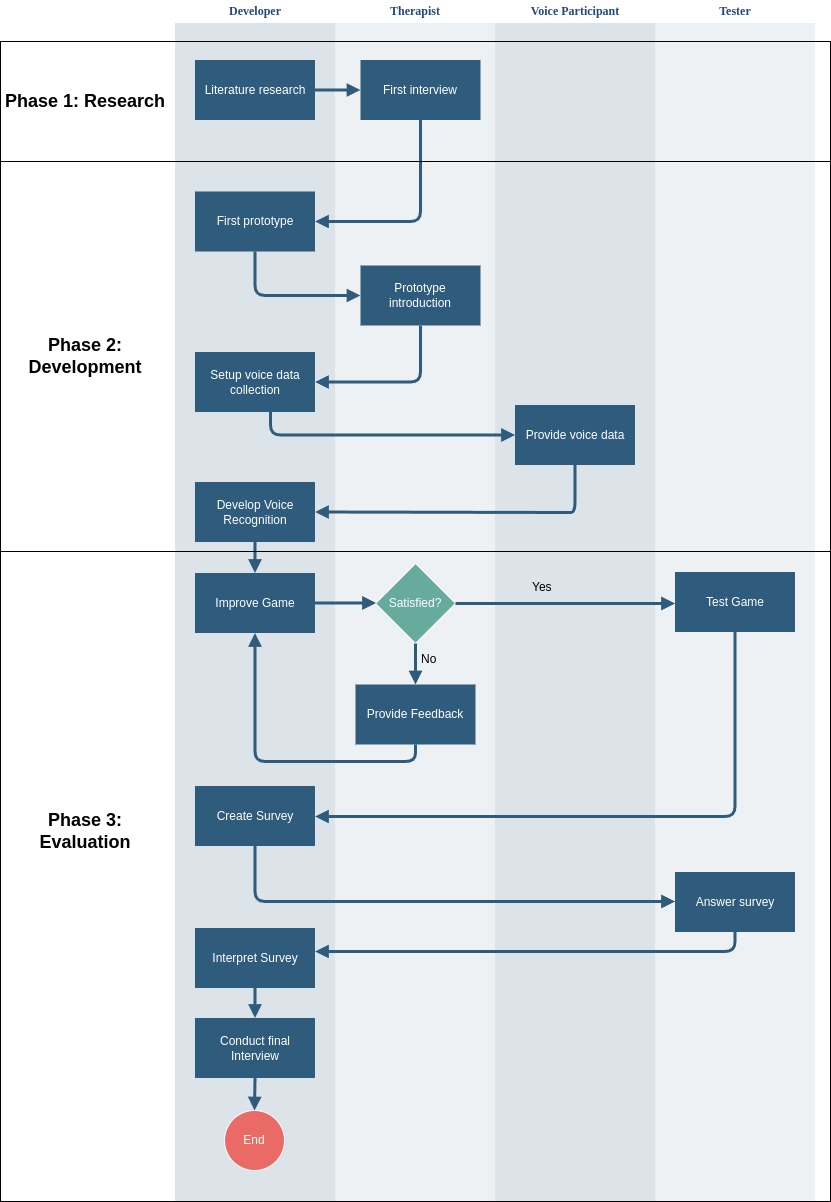
\includegraphics[scale=0.5]{Thesis_Process}
\end{center}
\caption{The thesis' course of action.}
\end{figure}

\section{General course of action}
\label{chap:coa}
\subsection{Phase 1: Research}
As with every thesis, the starting point will be a thorough literature research to determine the current state-of-the-art, as described in the previous section. This research consists of current Serious Games and their advantages and drawbacks as well as an introduction to three voice recognition softwares that could be used within the developed game. The research also includes fundamental theoretical background knowledge relevant to this thesis. Here, definitions for Serious Games and their subtypes, different types of speech impediments, the fundamental idea behind neural networks and voice recognition approaches, and the UCD process for developing products are given and elaborated on. Furthermore, an initial interview with a speech therapist will be conducted in order to gain basic domain knowledge in the field of speech therapy. Topics like the therapy process and common issues will be discussed, and first ideas regarding the development of the game are gathered. \\
It is worth mentioning that most of the state-of-the-art research described above was already conducted prior to the thesis' beginning. This unofficial "Phase 0", as one can call it, stems from a previous project which functioned as a feasibility study (see \cite{LEPaper}). More specifically, this study included state-of-the-art research regarding four Serious Games, three of which are also included in this thesis. This study does not, however, include as much theoretical background, especially regarding neural networks since this was not relevant at this time.

\subsection{Phase 2: Development}
Based on the input in the previous phase, a first prototypical version of the game is developed to showcase the core idea and gameplay. This prototype only consists of one level, as well as a mocked voice recognition algorithm. The prototype is then introduced to the therapist. This first feedback round with the therapist can be considered to be the most important one since the most pressing issues are likely to be mentioned in this step and implementing features in this stage of development can be expected to work rather smoothly since no changes on previous features have to be made. Once again, those steps were already taken beforehand \cite{LEPaper}, meaning the author was able to invest more time into the following processes. However, note that anything described below can be regarded as a novelty. \\
The next step is to implement an actual functioning voice recognition system. Since this system will include a neural network, domain-specific data will be gathered over the course of the next two months. The term domain-specific implies that current free data sets do not fit the game's requirements. This is due to two reasons: The game is meant to be played by German-speaking patients, thus limiting all possible training data to German as well, and the game heavily focuses on the pronunciation of single sounds or syllables, for which no data exists yet. The data will be collected via an online teaching platform that allows videos and audio files to be uploaded \cite{Flip}. Both author and therapist aim to recruit as much participants for audio data collection as possible. Most likely, a large percentage of participants will be recruited via personal communication and thus will probably stem from a similar location than author and therapist (Lower Austria/Vienna). This issue might become relevant later on as people in different regions tend to speak in dialect or pronounce certain phrases differently even when instructed to speak clearly. Thus, this participant sample might influence the voice model's performance later on. Afterward, this data will be used to train a custom voice recognition model which is then integrated within the game.

\subsection{Phase 3: Evaluation}
As a result of the previous phase, the game can now be played without needing to mock anything, although only one level is available at this point of time. Over the course of five additional iterations (six in total, if the first iteration within phase 2 is counted), each consisting of an interview and an improvement step, the game will be adapted accordingly until both therapist and the developer are satisfied. It is likely that core features will be implemented within the first iterations while later ones will probably consist of smaller changes instead. Afterward, the game will be distributed to the evaluation group, consisting of therapists, patients and volunteers, which are then asked to participate in a survey regarding their experience. Those volunteers will be recruited via personal communication and social media (i.e., Facebook groups) and will hopefully include multiple therapists and patients since they can be considered primary users of the game. As a last step, the survey's result are gathered and interpreted to get a final verdict of the game's reception and potential benefit for patients. Additionally, a final qualitative interview with the aforementioned therapist will be conducted in order to reflect on both the game's final state and its development process.


\section{Answering Research Questions}
To answer \emph{RQ1}, the methodology of \emph{prototyping} \cite{wilde2006methodenspektrum} is used. To do this, two artifacts are created: a \emph{requirement catalog} for Serious Games in speech therapy as well as a \emph{prototypical implementation} of the game. These two artifacts are developed and improved on using a \emph{user-centered-design} (UCD) pattern, meaning that relevant stakeholders (i.e., therapists) for this project are continuously introduced to the artifacts. Based on their opinions and recommendations, the artifacts are adapted accordingly until both the author and the stakeholders are satisfied with the result and RQ1 is answered. Within this thesis, a total of six iterations occurred. The first iteration was used to gain domain knowledge and to design a first working version (phases 1 and 2). Iterations 2-6 were then used to continuously improve on the prototype (phase 3). Naturally, the first iterations included more essential features while later iterations focused more on fixing issues in existing features and performing smaller functional changes.

Answering \emph{RQ2} is done by conducting interviews with the therapist in order to evaluate which game data could be useful for further rehabilitation. To be precise, the methodology of \emph{semi-structured interviewing} \cite{wilde2006methodenspektrum} is applied. Most of the relevant information for RQ2 was gathered during the first interview, with the following interviews adding only minor changes.

\emph{RQ3} is answered by conducting a \emph{field study} \cite{wilde2006methodenspektrum}. Once the development of the game is finished, it is distributed to a evaluation group, which play the game for one month. Afterward, each participant completes a short survey regarding their experience with the game and how it compared to classical therapy. Due to the rather small target audience and accessibility to the author, the evaluation group does not only include therapists and patients but also volunteers which evaluated the game even though they could not be considered part of the target audience. The testers have to rank various aspects of the game and classical therapy on a scale from 1 to 10 which is then evaluated to discover whether the game provides a statistically measurable benefit. Within this thesis, the term \emph{benefit} includes two measurements: \textbf{entertainment} and \textbf{subjective improvement}, meaning how much does the patient think he has improved on his vocal capabilities by playing the game. To determine a statistically significant difference, the survey data is first analyzed and evaluated whether it is normally distributed using the \emph{Shapiro-Wilk test} \cite{shaphiro1965analysis} as, in general, this method is considered best practice as of now \cite{hernandez2021testing}. This step is crucial since, depending on the result, an appropriate test method can be selected. Evaluating the data showed that for all pairwise comparisons between the game and classical therapy, a normal distribution can be assumed. Thus, in order to measure a statistically measurable benefit, a \emph{pairwise t-test} is performed \cite{maxwell1980pairwise}.

\section{Declaration of personal interviews with experts}
This section aims to shed some light on the expert that played an integral part while creating this master thesis due to their superior field knowledge. Therefore, this section credits her for her contribution. \\

The expert from which the author derived most of his logopedical knowledge is a speech therapist working in Lower Austria. She finished her degree in "Logopedics, phonetics and audiology" in 2019 and has since worked mainly with children suffering from speech impediments. 
%Most of her patients are between four to six years of age, although she also works with children up to 15 years. Such patients usually suffer from some kind of orofacial dysfunction caused by braces. Typically, the therapy process lasts about 15 weeks depending on the severity of the patient's impediment. As of now, the therap
Her knowledge of the most common issues when practicing with her patients as well as the therapy process proved to be an integral part of the game design process within this thesis. For the rest of this thesis, whenever the term \emph{therapist} or \emph{speech therapist} is used to describe therapy related topics, it is this person that is being referenced. \\

For the scope of this thesis, this therapist was the only one which was actively involved within the development process. Naturally, this may prompt the question on why not more therapists were involved. While including more therapists allows for collecting more diverse feedback and thus may result in a better end result, working with only one therapist also provides some advantages. For once, proposed feedback can be implemented very fast since no compromises between conflicting feedback of multiple therapists have to be made. Thus, the implementation of a working prototype for the Serious Game can be done incredibly fast. Furthermore, by only including one therapist, UCD-iterations can be planned and executed highly flexible since organizing a meeting with one person is vastly easier than it is with multiple therapists which all have different time schedules. Admittedly, those multiple therapists could have been met in different meetings but then again the issue of conflicting feedback mentioned above rises. Note, however, that multiple therapists were indeed included during the evaluation phase of the thesis (see Chapter \ref{chap:eval}). Thus, additional recommendations for possible future work including the Serious Game could be gathered while still providing an efficient development process.

\section{Other Participants}
During the course of this thesis, additional participants were asked to contribute by either providing voice data during phase 2 or by evaluating the finished Serious Game in phase 3. To credit their participation as well as give context to the selected cohort, this section is dedicated to them. For sampling, a combination of \emph{Purposive sampling} \cite{etikan2017sampling} and \emph{Snowball sampling} \cite{berndt2020sampling} was used; in a first step, the author individually selected a small group of suitable participants. These participants were then instructed to recruit further suitable candidates they knew according to the author's requirements (i.e. participants have to have good pronunciation for voice gathering). This approach was chosen in order to involve as many participants as possible while assuring relatively high participant suitability. Tables \ref{tbl:voice} and \ref{tbl:tester} provide a short overview of the involved people.

\begin{longtable}[h]{|c|c|c|c|c|}
\hline
\textbf{\makecell{Participant \\ID}} & \textbf{Age} &  \textbf{Gender} & \textbf{Occupation}  & \textbf{Recruitment method}\\ \hline
P1 & 20-30 &  Female & Speech therapist & Purposive sampling \\ \hline
P2 & 20-30 &  Male & Student & Purposive sampling \\ \hline
P3 & 20-30 &  Female & Student & Purposive sampling \\ \hline
%R4 & Sentence level &  Levels that cover the sentence level exist. & yes \\ \hline
P4 & 20-30 & Female & Flight Attendant & Purposive sampling \\ \hline
P5 & 50-60 & Female & Psychiatrist & Purposive sampling \\ \hline
P6 & 50-60 & Female & Primary school teacher & Snowball sampling \\ \hline
P7 & 30-40 & Female & Primary school teacher & Snowball sampling \\ \hline
P8 & 20-30 & Female & Primary school teacher & Snowball sampling \\ \hline
P9 & 20-30 & Female & Primary school teacher & Snowball sampling \\ \hline
P10 & 30-40 & Female & Speech therapist & Snowball sampling \\ \hline
P11 & 20-30 & Female & Speech therapist & Snowball sampling \\ \hline
P12 & 20-30 & Male & Student & Snowball sampling \\ \hline




\caption{Participants for voice data gathering.}
\label{tbl:voice}
\end{longtable}

\begin{longtable}[h]{|c|c|c|c|c|}
\hline
\textbf{\makecell{Participant \\ ID}} & \textbf{Age} &  \textbf{Gender} & \textbf{Occupation}  & \textbf{Recruitment method}\\ \hline
T1 & 20-30 &  Female & Student & Purposive sampling \\ \hline
T2 & 20-30 &  Female & Speech therapist & Purposive sampling \\ \hline
T3 & 10-20 &  Male & Patient & Snowball sampling \\ \hline
%R4 & Sentence level &  Levels that cover the sentence level exist. & yes \\ \hline
T4 & 10-20 & Male & Student & Purposive sampling \\ \hline
T5 & 20-30 & Female & Student & Snowball sampling \\ \hline
T6 & 10-20 & Male & Student & Snowball sampling \\ \hline
T7 & 20-30 & Male & Physical therapist & Purposive sampling \\ \hline
T8 & 30-40 & Female & Primary school teacher & Snowball sampling \\ \hline
T9 & 20-30 & Female & Student & Snowball sampling \\ \hline
T10 & 40-50 & Male & Unknown & Snowball sampling \\ \hline
T11 & 20-30 & Male & Speech therapist & Snowball sampling \\ \hline
T12 & 30-40 & Female & Primary school teacher & Snowball sampling \\ \hline
T13 & 30-40 & Female & Primary school teacher & Snowball sampling \\ \hline
T14 & 20-30 & Male & Speech therapist & Snowball sampling \\ \hline
T15 & 20-30 & Female & Primary school teacher & Snowball sampling \\ \hline
T16 & 20-30 & Female & Speech therapist & Snowball sampling \\ \hline
T17 & 30-40 & Male & Primary school teacher & Snowball sampling \\ \hline
T18 & 30-40 & Female & Student & Snowball sampling \\ \hline
T19 & 40-50 & Female & Primary school teacher & Snowball sampling \\ \hline



\caption{Evaluators for Serious Game evaluation.}
\label{tbl:tester}
\end{longtable}

\chapter{Results}
\label{chap:results}
The following chapter elaborates on the results of this master thesis. This includes the iterative development approach, an extensive description of the requirements of the Serious Game as well as its architecture, and concludes with a summary of the evaluation phase of this thesis.

Even though the main capabilities of the Serious Game are going to be discussed further in Section \ref{sec:Features}, a brief summary of the core aspects of the game will be presented immediately. The Serious game is a 2D platformer which was developed using the Unity Game Engine. In it, the player controls an avatar which tries to jump from platform to platform until the goal at the top is reached. In order to jump, however, the player has to issue certain sounds or words correctly.


%\section{Game Description}
%The Serious Game is a 2D platformer which was developed using the Unity Game Engine. The main gameplay is pretty simple: The player controls an avatar which tries to jump from platform to platform in order to reach the goal at the top. However, unlike a normal platform game, the player cannot move the avatar using keyboard inputs but rather has to issue certain sounds or words to make the avatar jump to the next platform. These sounds can differ from platform to platform and between different levels. After 10 jumps, the avatar reaches the top and the level is completed. Additionally, the player can opt in to enable the lava feature. This adds a failing condition to the game: the lava rises constantly, and if the avatar is too slow on its ascend, it dies upon touching it.
%To aid the player, the game offers three means of support:
%\begin{itemize}
%\item Lip movement images: When struggling with the current jump, the game will display an image of the correct lip movement for the current jump. This can help the player in better articulating himself.
%\item "Listen" - Button: When pressing the button, the player can hear the currently wanted sound or word being said by either a therapist using pre-recorded audio files, or using Google's text-to-speech engine. This feature is especially relevant for players who have trouble reading, i.e., children or mentally impaired adults.
%\item "Skip" - Button: If the player continuously fails to pronounce the wanted sound correctly, he can skip the current jump by pressing this button.
%\end{itemize}
%Additionally, the Serious Game features a child-mode. This mode replaces the lip movement images with other, more child-friendly sound cards. Last but not least, each level can be customized by the therapist using an editor. This, however, will be discussed in more detail in the next sections. 
%\\
%Before elaborating on the features of the final game, the next sections aim to highlight the development process behind it. As previously mentioned, the game was developed using a UCD-approach, which will be elaborated on now.
\section{Iteration 1}
The first iteration acted as an introduction for both author and therapist; the author presented a rough prototype of one level of the game, which included many mocked-up functionalities, to the therapist. This was done so that the therapist would get a rough idea of the proposed main gameplay mechanic on which the whole game would build upon later on. During this stage of development, adapting the gameplay would have been rather quick and easy to do if necessary. On the other hand, the author gained valuable domain knowledge regarding speech therapy as well as some first concrete feature recommendations for the game from the therapist, which are both listed below:
\begin{itemize}
\item \textbf{Logging capabilities:} The therapist wanted to measure patient progress in a meaningful way. To achieve this, two new logging metrics were included: \textbf{Average sound completion time} (AST) and \textbf{most common mistake} (MCM). AST states how long a patient needed to correctly pronounce a given sound. To determine this metric, the time the player needs to complete one single jump is measured, linked to the target phrase and stored in an external .csv file for later usage. Ideally this value decreases over time as the patient improves. MCM on the other hand, simply states, given a specific sound or word, what was the most common mistake for that sound? For example, if the patient has to say "t" but instead utters three times "d" and one time "k", the MCM for "t" would be "d". The aim of MCM is to assist the therapist in adapting therapy content and exercises depending on current pronunciation issues.

\item \textbf{Multiple sound stages:} Given a sound, the therapist wanted the levels of the game to continuously build up and integrate this sound over various stages  (phonetic, syllabic and word). By default, those stages should be increasing in difficulty, meaning single vocals or syllables should be exercised prior to whole words. Additionally, including a fourth stage into the game was considered, but ultimately discarded. The fourth stage would have included whole sentence the player has to speak. However, many therapists regard this stage to be rather optional since the learning difference between speaking one or even multiple words and whole sentences is slim and thus it is often not necessary to include sentences within the therapy process \cite{proestler2023}. Normally, patients master this stage on their own within day-to-day interactions.

\item \textbf{Syllabic construction:} When constructing syllables for the syllabic stage (i.e., the second stage in the therapy process after practicing single sounds), the following order of difficulty should be considered:
\begin{itemize}
\item Consonant + Vocal (CV): This combination is the easiest, as the patient has supple time to pronounce the "short" consonant at the start and simultaneously can elongate the vocal at the end. Such syllables can therefore be included in the first syllabic levels.
\item Vocal + Consonant (VC): The patient is still able to elongate the vocal, but has limited time for the consonant.
\item Vocal + Consonant + Vocal: Same as before, but with an added consonant.
\item Consonant + Consonant + Vocal (CCV) or CCVC: the hardest type of syllables as almost each sound has to be precise and short.
\end{itemize}
\item \textbf{No local synonyms:} When practicing whole words, those words must not have widely known and used synonyms in other parts of the country or even cross-country (i.e., Austria and Germany has many such words). This is useful as to not confuse the patient unnecessarily and is especially useful for patients that either do not speak German natively or also suffer from Aphasia since for such patients, semantic understanding of words or sentences is already compromised.
\item \textbf{Optional fail condition:} Some patients thrive on competitiveness. While the Serious Game is meant to be played as a singleplayer game, this does not infer that competition cannot be present. Thus, the idea arose to include an optional failing condition within the game's levels. This will be later on realized by implementing a lava floor that slowly rises and, if it touches the avatar, would fail the level instantly.  
\item \textbf{Lip movement images:} In contrast to the previous recommendation, other patients might need or want more assistance when playing. As a first measurement, the inclusion of lip movement images was proposed. These images illustrate how the patient must form their lips and circulate air in an out of his or her mouth in order to produce the desired vocal. These images are to be shown whenever the patient has issues uttering a certain sound.
\end{itemize}
In addition to the features listed above, currently mocked functionalities (i.e., the voice recognition and jump movement) had to be implemented as well since the therapist was satisfied with the main idea of the game. This implied that voice data had to be collected from now on, meaning both therapist and the author were additionally tasked to recruit many volunteers who were willing to contribute small audio recordings of them saying short phrases. All recordings were initially uploaded to a third-party platform called \emph{Flipgrid} \cite{Flip}, from which the author would retrieve and process them later on (see \ref{sec:playLevel}). Thus, this iteration took the longest to complete.
\section{Iteration 2}
The second iteration began as soon as all previously mentioned recommendations were addressed. Some previously mocked functionalities were implemented as well, although the voice recognition component was still not replaced. This was because at this point of time, only few audio responses were collected and thus a customized model could not be created yet. However, as a first step, the mocked voice recognition was already replaced with a non-customized model, which was not ideal but still an improvement. The interview with the therapist, in which the current state of the game was shown again, resulted in yet another wave of possible improvements:

\begin{itemize}
\item \textbf{Specific sound restrictions:} Depending on the exercised sounds, some additional restrictions may apply. For example, in German, the sound "r" is never accentuated at the end of a syllable or word. This does not mean that there are no words ending with "r", but rather that those words are spoken in a way that they do not omit the sound in normal day-to-day conversations. In the case of "r" this means, that the game has to avoid using words or syllables ending with "r" altogether, if practicing "r" is the current goal. The therapist provided a whole list of such cases which was considered during later stages of development.
\item \textbf{Level Customization:} Since every patient struggles with different sounds, it does not make sense to let them all practice the same sounds. Thus, the therapist proposed that there should be a possibility to create own \textbf{categories}. A category consists of 14 levels by default which can each be customized by the therapist. Furthermore, for each category, the therapist must choose one \textbf{main sound} (i.e., the sound which is practiced) and at least one \textbf{distracting sounds} (i.e., sounds that provide contrast to the main sound). For each level, the therapist can additionally select the stage (phonetic, syllabic or word), where the sound appears in regard to specific sound restrictions as mentioned above (i.e., start, middle, or end of syllable/word), and if distracting sounds are included. By default, the order of levels progresses in difficulty, meaning phonetic stage levels come before syllabic and word levels, but this order can be customized by the therapist as well if necessary. For this feature, both therapist and author sketched a rough workflow (see Figure \ref{fig:prototype}).
\begin{figure}
\begin{center}
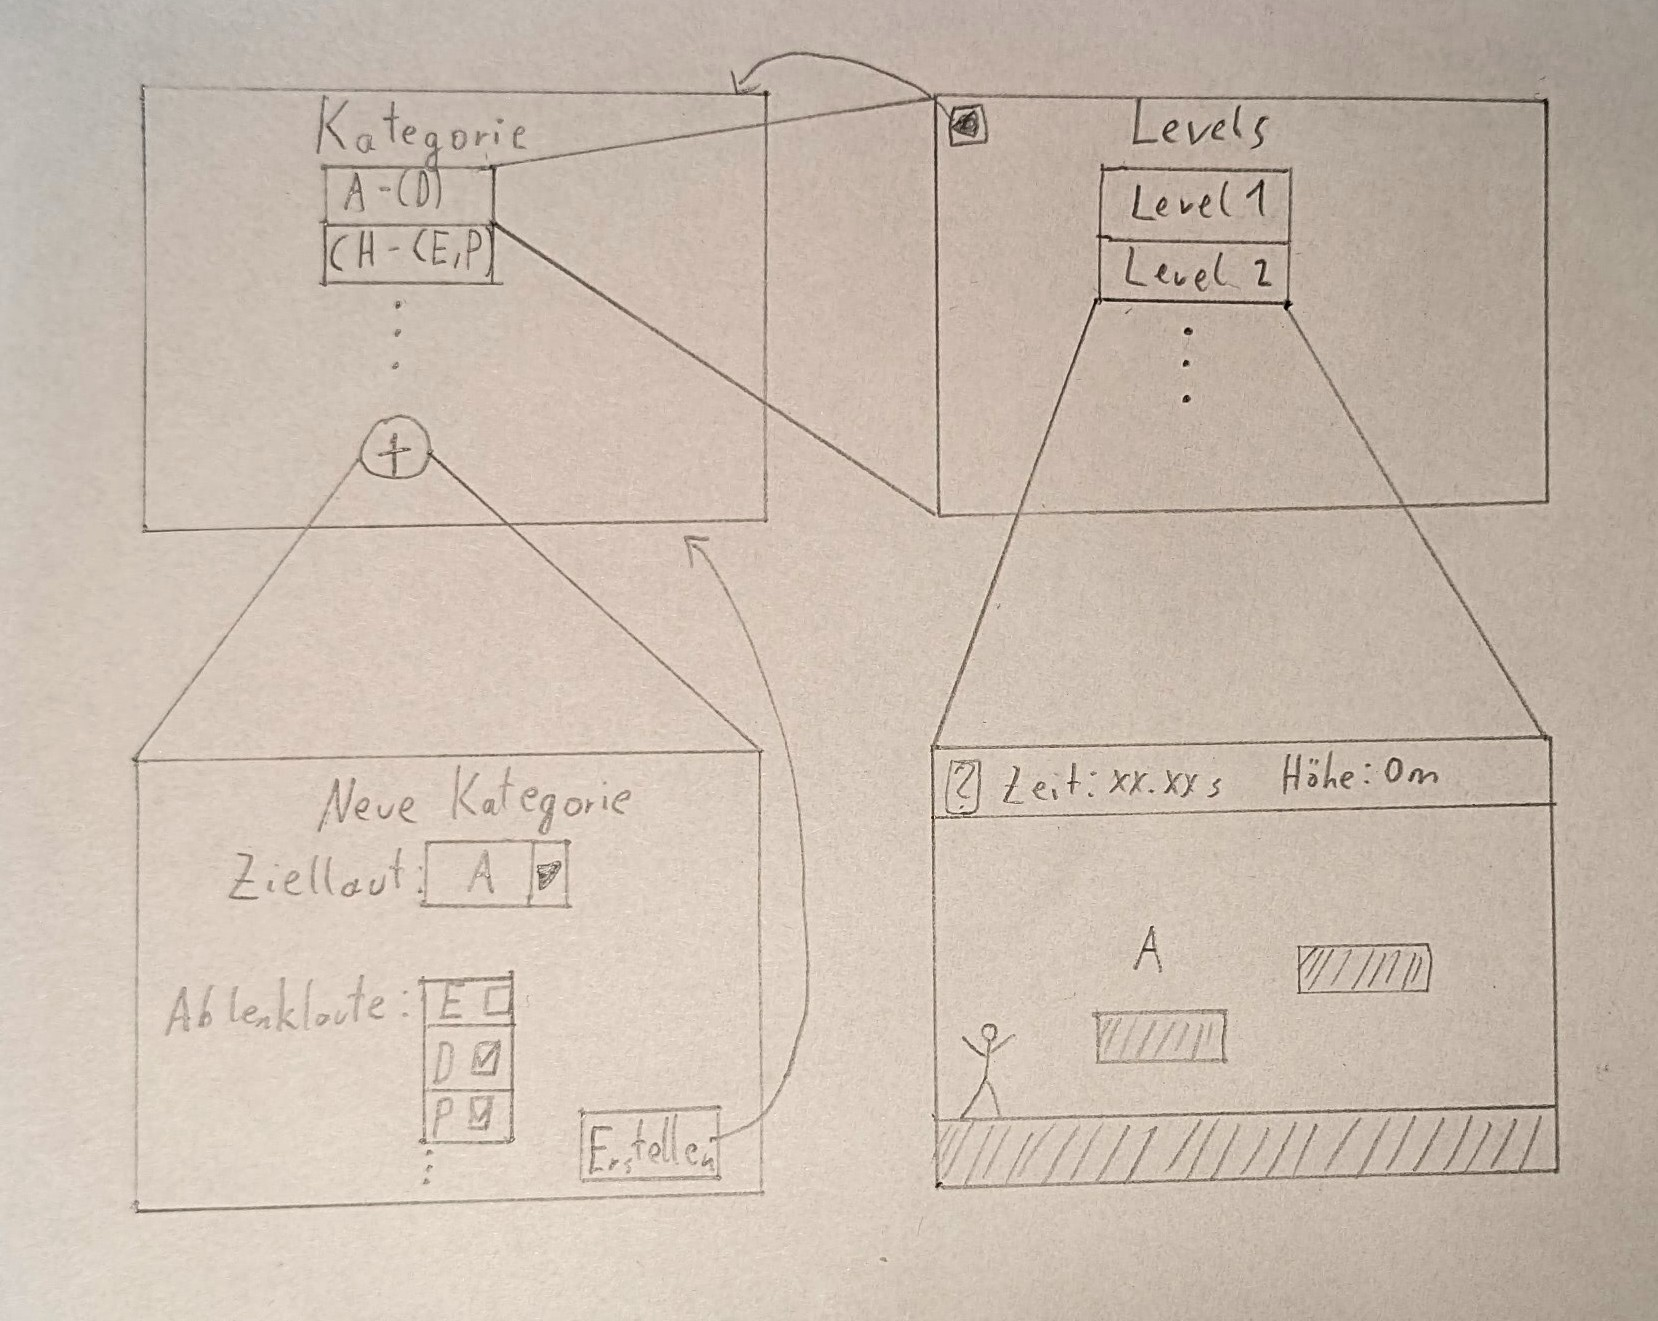
\includegraphics[scale=0.2]{Prototype}
\end{center}
\caption{Rough sketch for category navigation.}
\label{fig:prototype}
\end{figure}
\item \textbf{Level High scores:} For each level, there are two different kinds of scores. \textbf{Accuracy} dictates how many target phrases the patient pronounced correctly on the first try and \textbf{Time} states how long the player needed to complete the level. The best score in each category is visible from the level selection screen. Additionally, when completing a level, the scores of the current playthrough can be viewed as well.
\item \textbf{Level Progression:} In order to progress from one level to the next, the player has to not only complete the previous level, but do so with a high enough accuracy score. The threshold can be configured in the main menu and by default is set to 80\%. Including this aspect aims to promote quality over quantity for the patient playing the game. For example, if the patient gets the task of unlocking the next 3 levels until next week by the therapist, he can not simply rush through the levels in order to complete his goal. Rather, he has to qualitatively practice with each level to achieve his goal.
\item \textbf{Speech Button:} A button which when pressed voices the currently sought phrase has to be added. This can further aid children which cannot yet read or patients who lost this ability due to an accident or disease. Ideally,the pronunciation provided by this feature should mimic the expected input by the patient. To somewhat ensure that this was the case, the therapist provided multiple audio recordings of herself correctly pronouncing phrases, although many syllables had to be auto-generated due to the massive amount.
\item \textbf{Child Mode:} In child mode, the game displays child-friendly sound cards for the currently needed phrase. This could be, for example, a drawing of a snake for "s" as this is the sound the snake makes. Implementing this feature should make the game more appealing to children and by using sound cards also provide additional aid. These sound cards replace the lip movement images which would normally be displayed.
\end{itemize}
\section{Iteration 3 and 4}
Since both iterations were rather small, mentioning them together seems like a practical idea. Note that the iterations were so short due to the speech therapist not providing more feedback. When showing the current prototype which resulted from iteration 2, the therapist was so positively surprised that only few immediate improvement recommendations came to mind. Thus, iteration 3 mainly consisted of changing naming conventions and slightly adapting the child mode functionality. Additionally, work on the customized voice recognition component was finally resumed as sufficient data was collected and practically no new data was contributed. When introducing the next prototype, however, the therapist had enough time to think of beneficial additions for the Serious Game. Therefore, iteration 4 again brought some more impactful recommendations:

\begin{itemize}
\item \textbf{Skip Button:} When the player fails to input the correct phrase 3 times in a row, there has to be a possibility to skip the current phrase and go to the next one. Using this button does not raise the accuracy score for the level. This feature is meant to counter frustration and encouraging the player to keep trying.
\item \textbf{Remove levels:} When creating a new category, single levels are removable, bringing the number of levels of the category down. This feature is beneficial as the therapist might not need or want so many levels for one sound.
\item \textbf{Strictly limited word list:} The words that appear within the game are created randomly for each level, but stem from a small previously selected pool of words. This pool was created by the therapist herself and thus is suitable for therapy. For each word, a custom sound card that would be displayed along the word  if the game's child mode is enabled was added as well. Those sound cards were either taken from Madoo \cite{Madoo}, which is an online platform where german speaking speech therapists can both provide and download created therapy material without having to concern themselves about licensing issues, or even drawn by hand.
\end{itemize}
While those recommendations still include features that were present in the final prototype of the game, the importance of those features already declined when comparing them to previous iterations. This was to be expected and even desired, as this would make room for reviewing and potentially improving on previous features within the iteration.
\section{Iteration 5 and 6}
Once again, both of those iterations were not big enough to fill their own section, thus they are combined into one. Iteration 5 consisted only of the ability to remove previously created categories and iteration 6 only saw the addition of tool-tips for menu entries. Additionally, previous features were reviewed and slightly adapted as well. Last but not least, the possibility of porting the game to multiple devices and operating systems (i.e., Windows, Linux or Android) was explored, but ultimately it was decided that the focus was to stay on one platform alone. While Unity provides a built-in possibility to compile games suitable for various platforms, the author believes that additional work is required to make the game polished enough for mobile use. Rather than investing resources in this endeavor, the decision was made to allocate all effort into one version of the game.
\section{Requirements}
\label{sec:Features}
As a result of the previously mentioned iterations, the requirement catalog below was created. Each requirement consists of an ID, which is used for referencing later on, a name, a short description, an indicator whether the requirement is optional, an importance evaluation and in which iteration it has been implemented. A requirement's importance can range from 1 to 10, with 1 being the least important evaluation and 10 implying that the requirement must be present within the game at all costs. The importance of each requirement came from a subjective evaluation from both the author and the therapist. These requirements were afterwards summarized into five Use-Cases (see  Figure \ref{fig:UseCase}). This section will further elaborate on this use-cases and their challenges.

\begin{figure}
\begin{center}
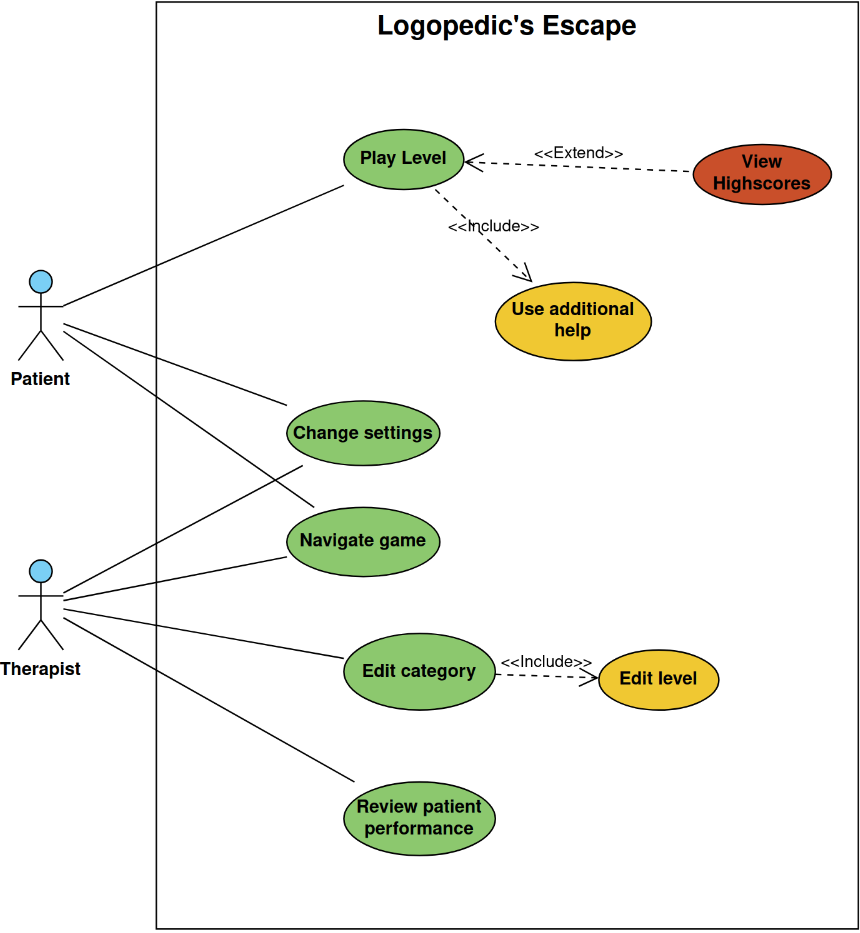
\includegraphics[scale=0.5]{LE_UseCase}
\end{center}
\caption{The Use-Case diagram for the game.}
\label{fig:UseCase}
\end{figure}

\begin{longtable}[h]{|p{.05\textwidth}|p{.15\textwidth}|p{.25\textwidth}|p{.10\textwidth}|p{.15\textwidth}|p{.10\textwidth}|}
\hline
\textbf{ID} & \textbf{Name} &  \textbf{Description} & \textbf{Optional}  & \textbf{Importance (1-10)} & \textbf{Iteration} \\ \hline
R1 & Phonetic level &  Levels that cover the phonetic level (only sounds) exist. & No &10 & 1 \\ \hline
R2 & Syllable level &  Levels that cover the syllable level exist. & No &10 & 1 \\ \hline
R3 & Word level &  Levels that cover the word level exist. & No & 8 & 1 \\ \hline
%R4 & Sentence level &  Levels that cover the sentence level exist. & yes \\ \hline
R4 & Voice control &  The avatar must be able to move by only using one's voice. & No & 10 & 3 \\ \hline
R5 & Voice recognition &  The recognized voice input must be displayed back to the user. & No & 8  & 4\\ \hline
R6 & Avatar animation &  The avatar's movement must be animated. & No &7 &1\\ \hline
R7 & Start screen &  A start screen must exist & No & 7 &1\\ \hline

R8 & Level overview &  A level overview menu must exist. & No & 6 &1\\ \hline

R9 & Background music &  Background music exists. & No & 6 &1\\ \hline

R10 & Animation music &  Animation music exists. & No & 6 &1\\ \hline
R11 & Stress component &  A stress component (failing condition) exists within a level & Yes & 3 &1\\ \hline
R12 & Lip movement image &  An image of the correct lip movement pops up if the patient fails repeatedly (phonetic level). & No & 6 &1\\ \hline
R13 & Required input &  The required input to continue is visible. & No & 10 &1\\ \hline
%%R15 & Word image &  An image of the currently sought word is visible (word level). & Yes \\ \hline
R14 & Info screen &  An info page regarding information about the game and its target group is visible. & Yes & 1 &1\\ \hline
R15 & Audio config &  Configuration of audio volume is possible. & Yes & 3 &1\\ \hline
%R18 & Level performance rating &  A rating of the player's performance within a level exists (i.e. 1-3 stars). & Yes \\ \hline
R16 & Data Log &  Logging of the player's performance on each level exists. & Yes & 8 &1\\ \hline
R17 & Child Mode &  A child mode which swaps lip movement images with sound-cards exists & Yes & 6 & 3\\ \hline
R18 & Pre-defined word list &  The words generated in word levels have to stem from a pre-defined list & Yes & 6 & 4\\ \hline
R19 & Skip-Button &  A button to skip the current jump exists. & No & 4 & 4\\ \hline
R20 & Listen-Button &  A button that when pressed reads out the current sound exists. & No & 4 & 4\\ \hline
R21 & Record-Button &  A button that when pressed starts recording the player exists. This feature presents an additional way of recording that does not need a keyboard & Yes & 3 & 6\\ \hline
R22 & High score-Time & For each level, the best time is visible & Yes & 7  & 2\\ \hline
R23 & High score-Accuracy &  For each level, the highest accuracy is  visible. & Yes & 7 & 2\\ \hline
R24 & Level Creation &  New levels can be created by the therapist. & No & 8 & 2\\ \hline
R25 & Category Creation & New categories, which consist of multiple levels, can be created by the therapist & No & 8 & 2\\ \hline
R26 & Category Customization: Sounds & The sounds which can be used for the category are selectable. This includes the main and distracting sounds. & No & 8 & 2\\ \hline
R27 & Level Customization & The levels are customizable in regards of sounds used, the therapy stage and their position within syllables/words & No & 8  &2\\ \hline
R28 & Category Deletion & Created categories are removable. & Yes & 6 & 5\\ \hline
R29 & Multiple voice recognition softwares & Multiple voice recognition softwares are available. & Yes & 8 &5\\ \hline
R30 & Voice recognition selection &  The currently used  voice recognition is selectable. & Yes & 8 &5\\ \hline



\caption{Requirements for \emph{Logopedic's Escape}.}
\label{tbl:requirements}
\end{longtable}

\subsection{Use Case: Play Level}
\label{sec:playLevel}
This Use-Case might be the most important one in order for the prototype to be classified as a Serious Game. Coincidentally, this Use-Case also covers the majority of the requirements (\textbf{R1-6, R9-13, R17-18, R29}), especially when also including the affiliated Use-Cases \emph{Use additional help} (\textbf{R19-21}) and \emph{View High scores} (\textbf{R22-23}). All of the mentioned requirements will be explained in more detail below. \\
For the patient to play a level, a level layout as well as its intended benefit must be defined. For that, all levels fall into one of three level types: \emph{phonetic, syllabic and word levels}.

\subsubsection{Phonetic level (R1)}
The phonetic levels are supposed to be the introduction to the game. As the phonetic plane is the first stage within therapy, making the first levels to address this therapy step seems reasonable. Note that those levels are not limited to only single letters, but also include compound letters, as long as they only produce a single sound (i.e., the combination 'sch' or 'ch' in German have a unique sound, making them viable for this stage). Furthermore, depending on whether the practiced sound within the level is a single vocal or a consonant, the difficulty of the level can vary. In general, vocals are easier to practice as the patient has the ability to prolong its pronunciation, while consonants are usually pronounced "short", making them more difficult. Obviously this classification can only be considered as a rough landmark, as each patient can perceive difficulties differently. Phonetic levels can additionally either consist of the \emph{target sound} (i.e. the sound that should be exercised) or include one or multiple \emph{distracting sounds} (i.e. sounds that aim to provide contrast to the target sound) with the latter being more the more difficult option.

\subsubsection{Syllable level (R2)}
Similar to the phonetic levels, the types of sounds (vocals or consonants) and their position within the syllable heavily influences its difficulty. Roughly speaking, shorter syllables are easier than longer ones, as are syllables that end with a vocal rather than a consonant. Thus, the default order of levels represents this trend as the difficulty gradually increases. Since the number of different syllables which include a predefined target sound is rather large. To provide some variability, syllables are thus generated at random when creating the level, all while respecting the various difficulty factors elaborated above. This means that, for example, an easy syllable level would feature short syllables for which the target sound is at the beginning of the syllable, while a more advanced level later might consist of longer syllables, all of which are randomly generated.

\subsubsection{Word level (R3)}
As the final stage of the level progression, word levels are supposed to be the toughest ones. However, not every word is equally difficult and suited for usage within the rehabilitation process. Again, shorter words are considered to be easier than longer ones. Instead of selecting words for the level from the pool of all words within the language, a smaller pre-selection was created with the help of the therapist. This pre-selection contains 123 words from which fitting words for the current level are selected at random. \\

Having defined the available level types, the next step is to implement its functionality. Starting with the patient input, the issue of R4-5 must be addressed.

\begin{figure}
\begin{center}
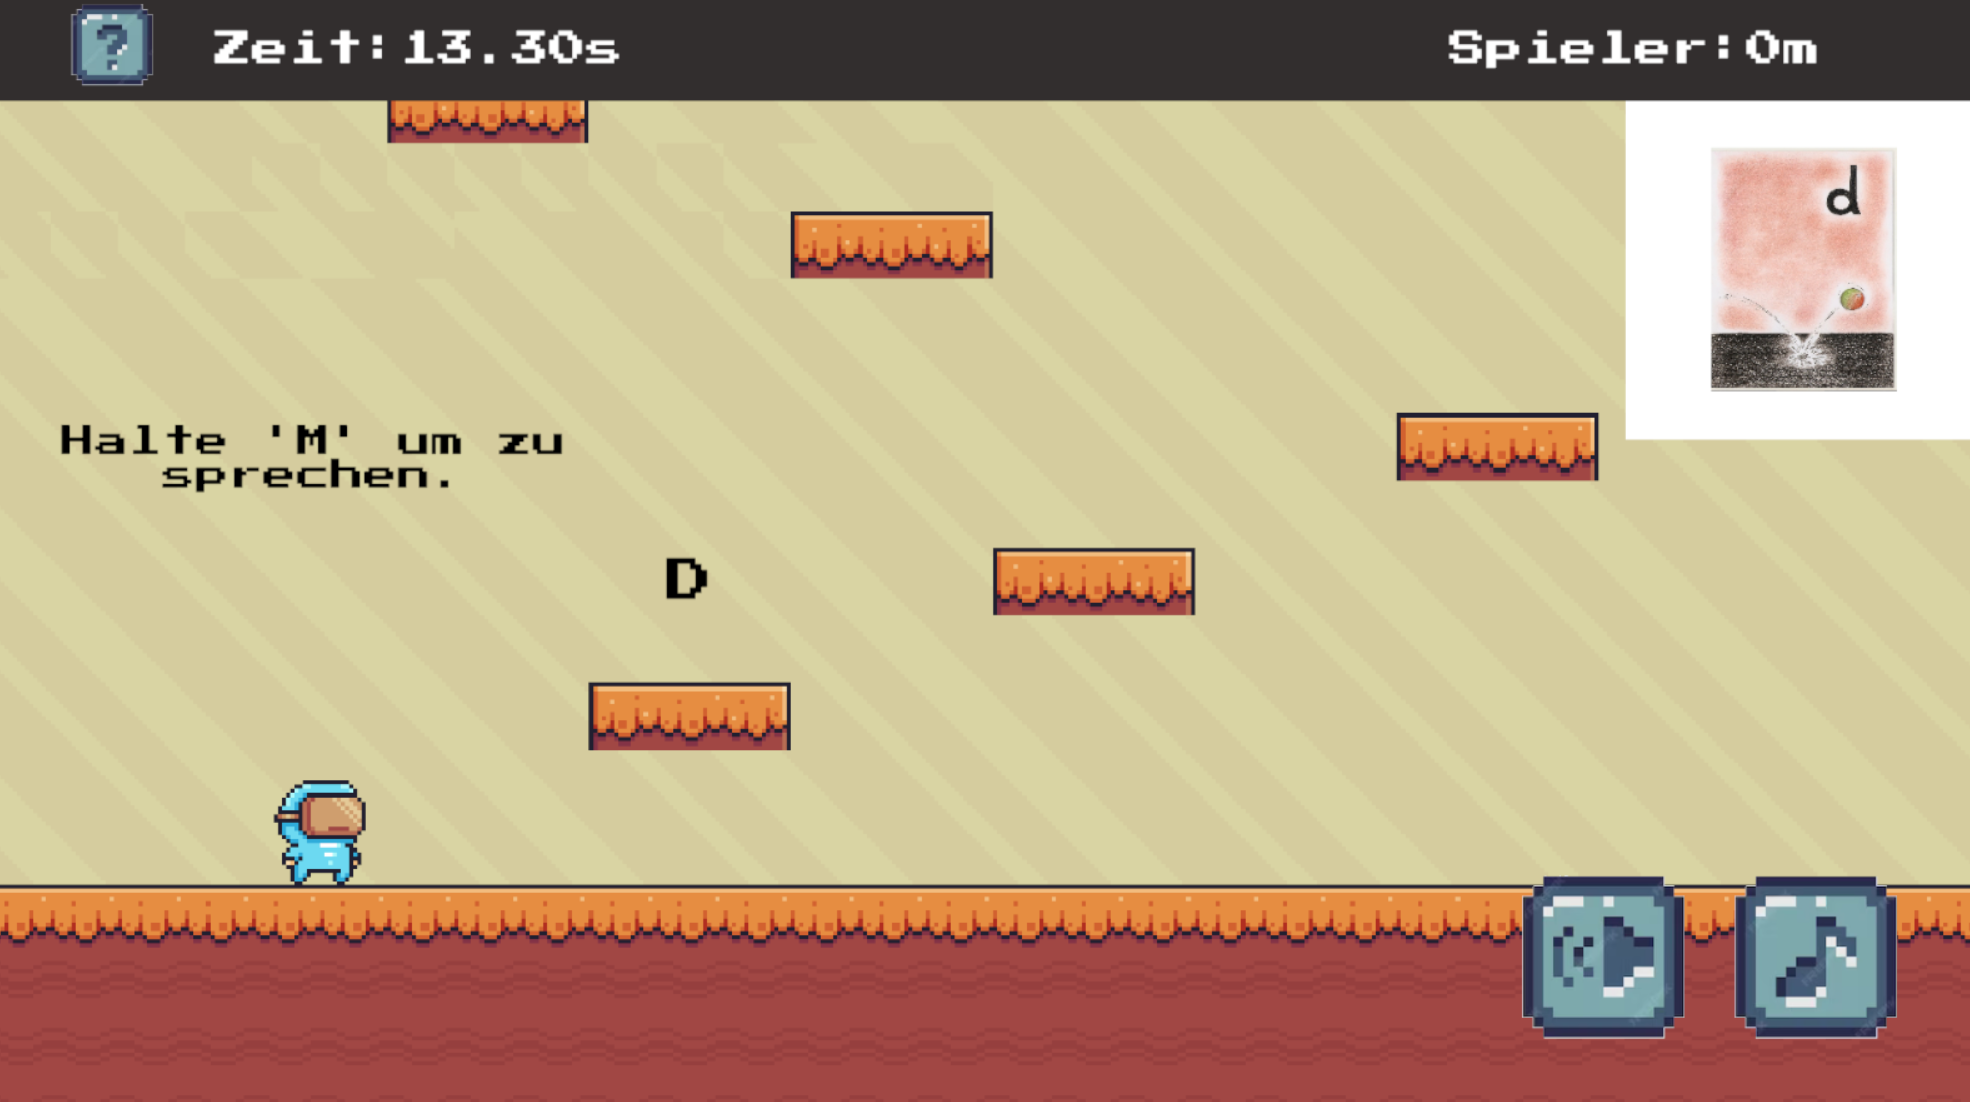
\includegraphics[scale=0.2]{LE_Level}
\end{center}
\caption{The level screen for a phonetic level. In this example, the currently sought phrase is the letter 'D'.}
\label{fig:UseCase}
\end{figure}
\subsubsection{Voice recognition (R5)}
Since the game is almost exclusively played via voice commands, this requirement was one of the most important ones in terms of gameplay. Ideally, the voice recognition component applied within this game has to fulfill the following criteria:
\begin{itemize}
\item It is able to correctly identify most words spoken. This should be a non-issue since almost all recognition software focus on whole word recognition, thus making existing solutions very fitting.
\item It is  able to correctly identify single sounds or syllables. This posed to be one of the two most pressing issues within this requirement, as this is something rather novel within the voice recognition sphere. Roughly speaking, this issue was addressed by collecting custom training data which was used to customize an existing voice model. The details of this process is elaborated below.
\item It is able to support German as this is the game's language. If future support for other languages is needed, however, this can be achieved rather straight-forward by simply replacing the voice recognition component. Additionally, in-game labels would have to be altered as well, but the recognition functionality itself would be rather straightforward to replace.
\item It is able to translate single words or sounds within five seconds. Anything longer would significantly impact the gameplay as the player would have to wait for too long. This was a second issue and will also be elaborated on further below.
\item It is available for free or a very low price since monetary resources for this thesis are scarce.
\item It requires no internet connection. This criteria is arguably the least important one since nowadays, access to the internet is practically provided at any time. However, having to rely on a constant internet connection might negatively impact translation time, thus impeding gameplay. Furthermore, patient data privacy is also an important factor to consider and while the author sees no initial harm in providing anonymous patient voice data for interpretation, one can never be too careful when patient data is involved. Thus, if a solution that requires an internet connection exists, it must perform exceptionally well compared to other alternatives in order to be a viable option. 
\end{itemize}

To satisfy these requirements, the author proposes four possible options which were open for discussion.

\paragraph{VoiceItt} As previously elaborated, VoiceItt is a voice recognition software specifically designed to aid speech impaired users. With its regional variation "VoiceItt-A", it even offers support for German-speaking users as well. However, there are some issues that need to be addressed. First and foremost, using VoiceItt is too expensive for the scope of this thesis. Additionally, the aim of the game is to train its players to correctly pronounce different sounds or words. Thus, using a recognition software that caters to the patient's slurred speech is rather counterproductive for therapy progress. It is therefore the author's firm belief that VoiceItt has no place within therapy but rather should be used for day-to-day communication if necessary.

\paragraph{Dragon NaturallySpeaking} Dragon NaturallySpeaking was developed by Nuance and is a dictating software for Windows. Depending on the environment (i.e., healthcare or legal dictation), different versions exist, with Dragon Professional being the most all-rounded one. While no scientific evaluation regarding its performance and accuracy exist, the consensus from customers is that Dragon NaturallySpeaking can be considered to be one of the better dictating softwares as of now. However, just like VoiceItt, Dragon NaturallySpeaking is too expensive to be considered a viable option within this thesis. Furthermore, it is also questionable whether it performs as well when tasked with identifying single sounds or syllables in contrast to whole words. Without knowing any details regarding the exact neural network learning process and the general infrastructure behind the Dragon products, the author suspects that recognizing single sounds or syllables is not an intended use case for this product and thus will most likely underperform in this regard. 

\paragraph{Whisper-API} In contrast, using Whisper is, at least for academic use, free of charge. With 680 000 hours of semi-supervised training data, Whisper managed to create a rather robust model. However, there are two major drawbacks when using the API-Version of Whisper. For one, making API-calls requires a constant internet connection, which violates the last requirement from the list above. While this alone does not automatically exclude it from consideration, it does negatively factor in within the decision process. The second, more serious issue, however, is that the number of API-calls that can be done within a minute is limited to five, meaning across all instances of the game, only five requests can be sent per minute. This issue makes the players wait too long and thus is the definitive criterion for exclusion. However, OpenAI also offers custom solutions to their API, meaning that depending on both acceptance and possible financial aid in the future, custom access which features more frequent calling capabilities might become feasible, making this option relevant again.

\paragraph{Whisper-Local} Instead of using Whisper's API, it is also possible to download and use local images of the neural network. These images can be downloaded in various sizes, with the smaller ones being faster but more inaccurate and the larger ones having reverse properties. For the scope of this thesis, the two smallest versions, which are called \textbf{tiny} and \textbf{base} are the only viable options since other versions take too much time to compute. Depending on the player's computer capabilities, these images could be switched within the game. The author believed this solution to be the best alternative, thus it is used within the game as of now. Additionally, by storing all audio data locally, a high degree of patient data privacy can be guaranteed. This makes current concerns regarding data privacy and the methods of keeping patient data private quite obsolete \cite{hathaliya2020exhaustive}.

\subparagraph{Adaption}
However, there is still one issue with using Whisper-Local that needs to be addressed. Since all Whisper images are trained to detect whole words and sentences, detecting single sounds or syllables proved to be a rather pressing issue. To mitigate this, the decision was made to take Whisper's solutions and further train them on more fitting test data to better detect single sounds. The test data consisted of over 200 recordings gathered from 11 different participants. Each participant had to record himself saying various phrases out of a pool of 51 pre-defined sounds and syllables.
The author does realize that this data set's size pales in comparison to other data sets used for speech recognition training. However, this was all that could be managed due to the limited audience range. It is important to note, that since the recognition  software has to be trained on only detecting correct pronunciations, the pool of possible participants was severely downsized as simple day-to-day speech is unfitting for therapeutic usages. This is especially true when dealing with single sounds or syllables since their pronunciation differs wildly within therapeutic context. Most importantly, when practicing such sounds, no additional sounds should be included (this is especially crucial when practicing consonants). Thus, those 11 participants solely consisted of either speech therapists which inherently know of this issue, or primary school teachers, which also are often confronted with similar situations.

\subparagraph{Adaption Process}
To gather the voice data, a pre-existing online tool was used. \emph{Flipgrid} \cite{Flip} is an online lecturing platform that allows educators to provide tasks to students. The students must then complete these tasks by recording short videos of themselves elaborating on the tasks and uploading it to the platform. For the scope of this thesis, this platform was used to gather the relevant voice data as joining a classroom and submitting the videos is made rather simple for the participants; each participant received an invitation link to join the classroom and, using their Google-Accounts, they were able to log into the platform within less than two minutes. For each sound or syllable a separate task was created. The participants then uploaded short videos of them saying the correct sound which is later on downloaded and further edited. Both the therapist and the author had an educator's access on the website, meaning they alone could create new tasks or edit uploaded responses. However, as of September 2024, Flipgrid is no longer available via their website. If future audio data collecting is needed and Flipgrid should be used, one has to use Microsoft Teams for this case as the Flipgrid functionalities are now included within it. For more information please refer to the official statement and instructions \cite{Flip}.\\
All responses are then downloaded and converted into audio files. For each file, an entry within a separate text file was added which stated the name of the file and its transcript. This process was done semi-automatically, as the initial labelling was done by hand, but both the file conversion and its corresponding text file insertion occurred by using a bash-script. Afterward, the Whisper Image was adapted using the gathered audio data. The adaption process is implemented in Python and follows the Whisper fine-tuning guide on the website "\emph{HuggingFace}" \cite{Huggingface}. Due to limited computation resources, however, this guide got adapted further (mainly reducing the number of recommended training iterations from 15,000 to 1,000 with 16 audio files per iteration). While this might seem as it would infer a substantial loss in model quality, one can argue against it in this particular case; since the gathered test data set is rather small, the author believes that the recommended amount of iterations can likely lead to model overfitting issues, thus producing better results in training, but making the model unusable within the application. Afterward, the resulting model is then converted in order to be usable within the game. More specifically, Unity's Whisper component \emph{WhisperManager} needs the model to be in the "\emph{ggml.bin}" \cite{ggml} format. As a quick explanation, ggml describes a machine learning library similar to \emph{PyTorch} or \emph{Tensorflow} \cite{ggmlInto}. It has recently gained more popularity and thus even the widely popular and highly compatible WhisperAI-port \cite{whisperCpp} uses it . Last but not least, this port has to be converted into a binary file to be compatible with Unity. To achieve this, the previously trained model gets converted with a python script \cite{WhisperConv}. 

\begin{figure}
\begin{center}
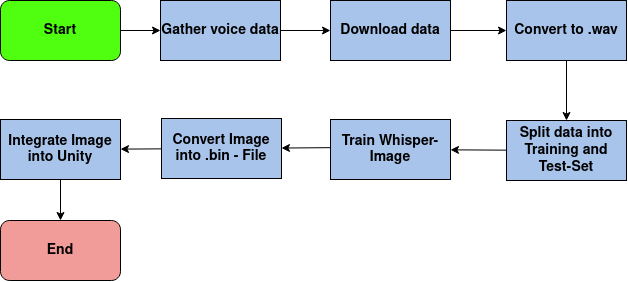
\includegraphics[scale=0.5]{Adaption_process}
\end{center}
\caption{The author's proposed adaption process for the Whisper Image for this thesis.}
\end{figure}

 
To complete the basic functionality of a level, only some small requirements are needed to be implemented: \textbf{R6}, \textbf{R9-10} and \textbf{R12-13}. \textbf{R6} describes the animation of the avatar's movement. While not crucial regarding functionality, it makes the game visually more pleasing and thus was included. The same can be said for the background- and animation music (\textbf{R9} and \textbf{R10} respectively). For these requirements, free assets available in the Unity Asset Store \cite{unityStore} have been used. \textbf{R13} states that the required voice input needed for the next jump has to be visible for the patient. This might not be the most exciting requirement, but it is crucial nonetheless. Finally, including lip movement images (\textbf{R12}) marks the first implemented aid for patients. 
\begin{figure}
\begin{subfigure}{.33\textwidth}
  \centering
  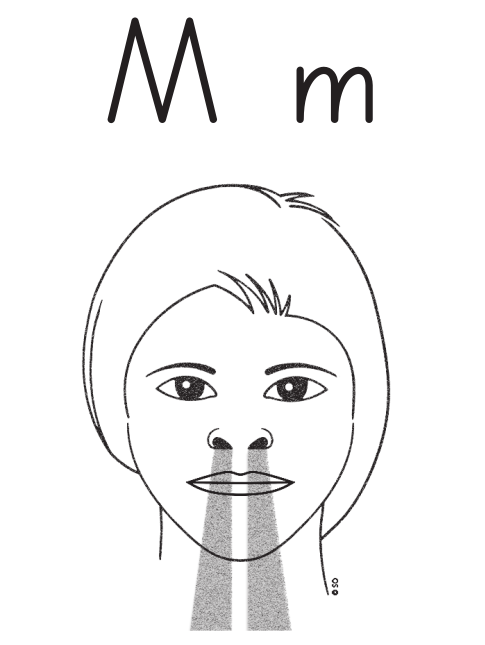
\includegraphics[width=.8\linewidth]{AM}
  \caption{m}
\end{subfigure}%
\begin{subfigure}{.33\textwidth}
  \centering
  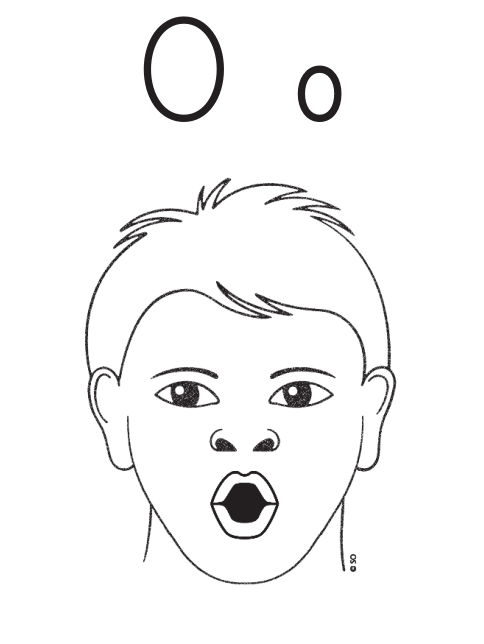
\includegraphics[width=.8\linewidth]{AO}
  \caption{o}
\end{subfigure}
\begin{subfigure}{.33\textwidth}
  \centering
  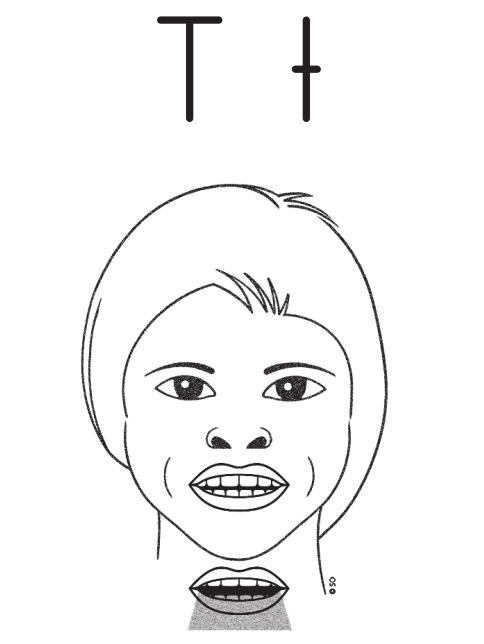
\includegraphics[width=.8\linewidth]{AT}
  \caption{t}
\end{subfigure}
\caption{Examples of lip movement images\cite{lipImages}. }
\end{figure}

Next up are requirements that are not essential for the basic functionality of the level, but instead are vital extensions which either improve user experience or therapy usability. Those requirements are: a stress component(\textbf{R11}), a child mode(\textbf{R17}), a pre-defined word list(\textbf{R18}) and the usage of multiple voice recognition softwares (\textbf{R29}).

\subsubsection{Stress component (R11)}
The addition of a stress component provides a challenge for more proficient or competitive players. To do so, a lava pool that slowly rises until it reaches the avatar was added within the game. While implementing the gameplay of this requirement was rather intuitive, stylizing the lava itself proved to be more of an issue than initially thought. Since the whole game is made with a pixel-esque look, the lava itself has to also look pixelated. However, in contrast to all other assets, the author could simply not find a fitting asset for free that fulfills these requirements. Thus, the lava asset was made and animated by the author himself. To do that, a rather new feature of Unity called a \emph{Shader Graph} was used. A Shader Graph is a visual pipeline for creating material textures. These textures can then be animated automatically, meaning drawing each animation frame by hand is not necessary. Instead, a mathematical function running in the background calculates all frames. This process proved to be very effective for this requirement. Additionally, if the need for re-textualizing were to rise in the future, this could be done quite easily with this approach. In contrast, if other game elements like the avatar or the platforms to jump on were to be re-styled, this would imply either searching for new available assets online again, or even drawing them by hand. Both are options which are obviously more time consuming than tweaking an existing Shader Graph.


\begin{figure}
\begin{center}
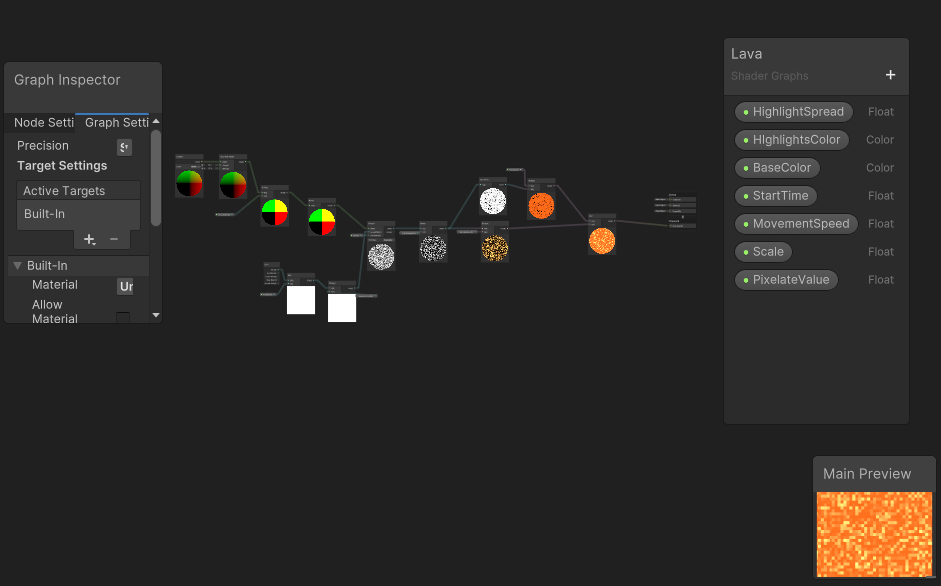
\includegraphics[scale=0.4]{LE_Lava}
\end{center}
\caption{The Shader Graph for calculating the lava texture.}
\end{figure}




\subsubsection{Child Mode (R17)}
Since the therapist has many children as patients, the idea of implementing an own child mode for the game came naturally as progress was made. The main issue on why a child mode is necessary in the first place are the lip movement images. While these are very useful within the therapy process as they visually instruct the patient on how to shape their mouth in order to utter certain sounds, children more often than not cannot make sense of these instructions. As an alternative, the therapist thus uses her own sound cards which describe the sound in a more child-friendly manner. For example, for the sound "s", the sound card depicts a picture of a snake which, when hissing, produces a very similar sound to "s".
This sound cards were not made by the author himself but rather taken from Madoo \cite{Madoo}, which is an online platform for speech therapists where an abundant amount of therapy material can be gathered free-of-charge. The only caveat one has by using those materials is that every product that includes those materials has to state that the images used are published using the Creative Commons License \textbf{CC BY-SA 4.0}\cite{License}. Since the License only applies to the sound cards and does not apply to the game and the game itself is not commercially used as of now, this was not an issue at all.
\begin{figure}
\begin{subfigure}{.33\textwidth}
  \centering
  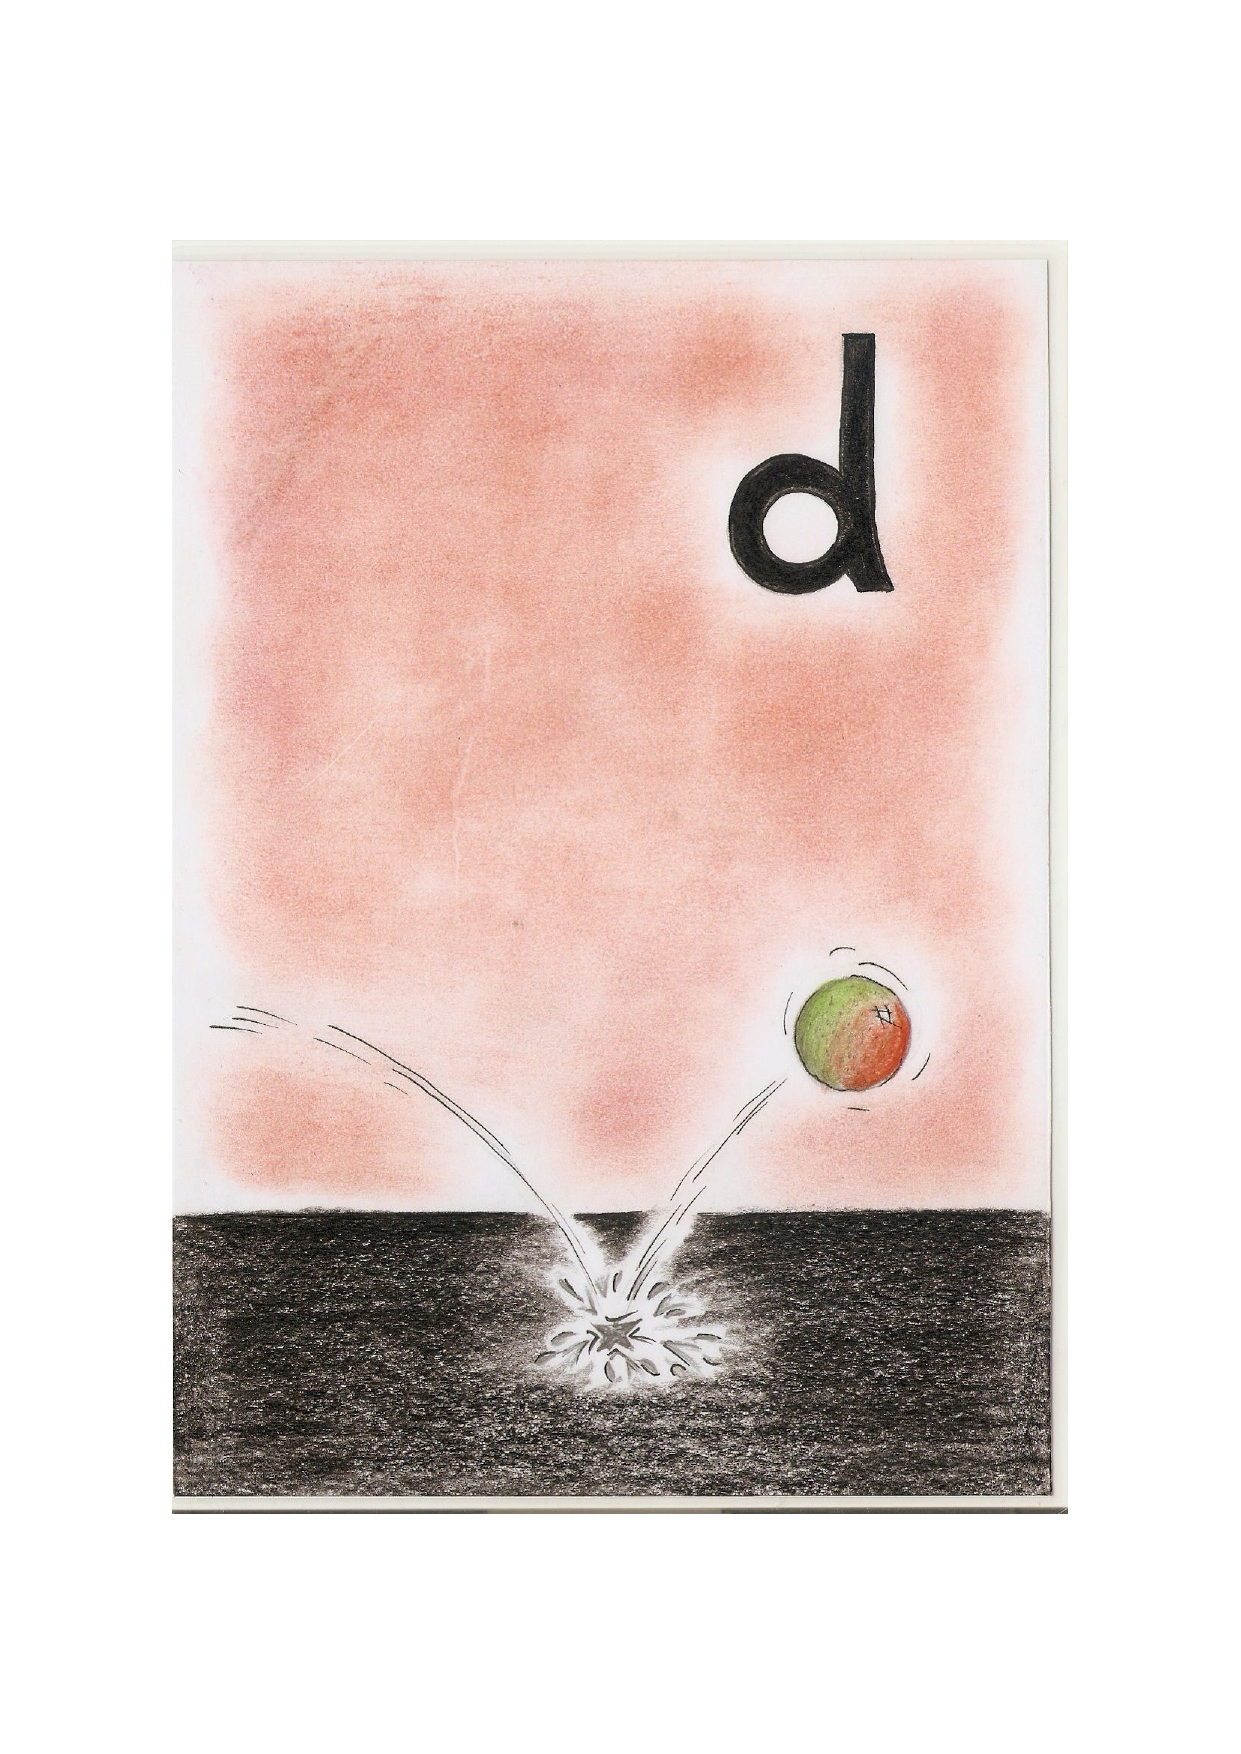
\includegraphics[width=.8\linewidth]{D}
  \caption{d}
\end{subfigure}%
\begin{subfigure}{.33\textwidth}
  \centering
  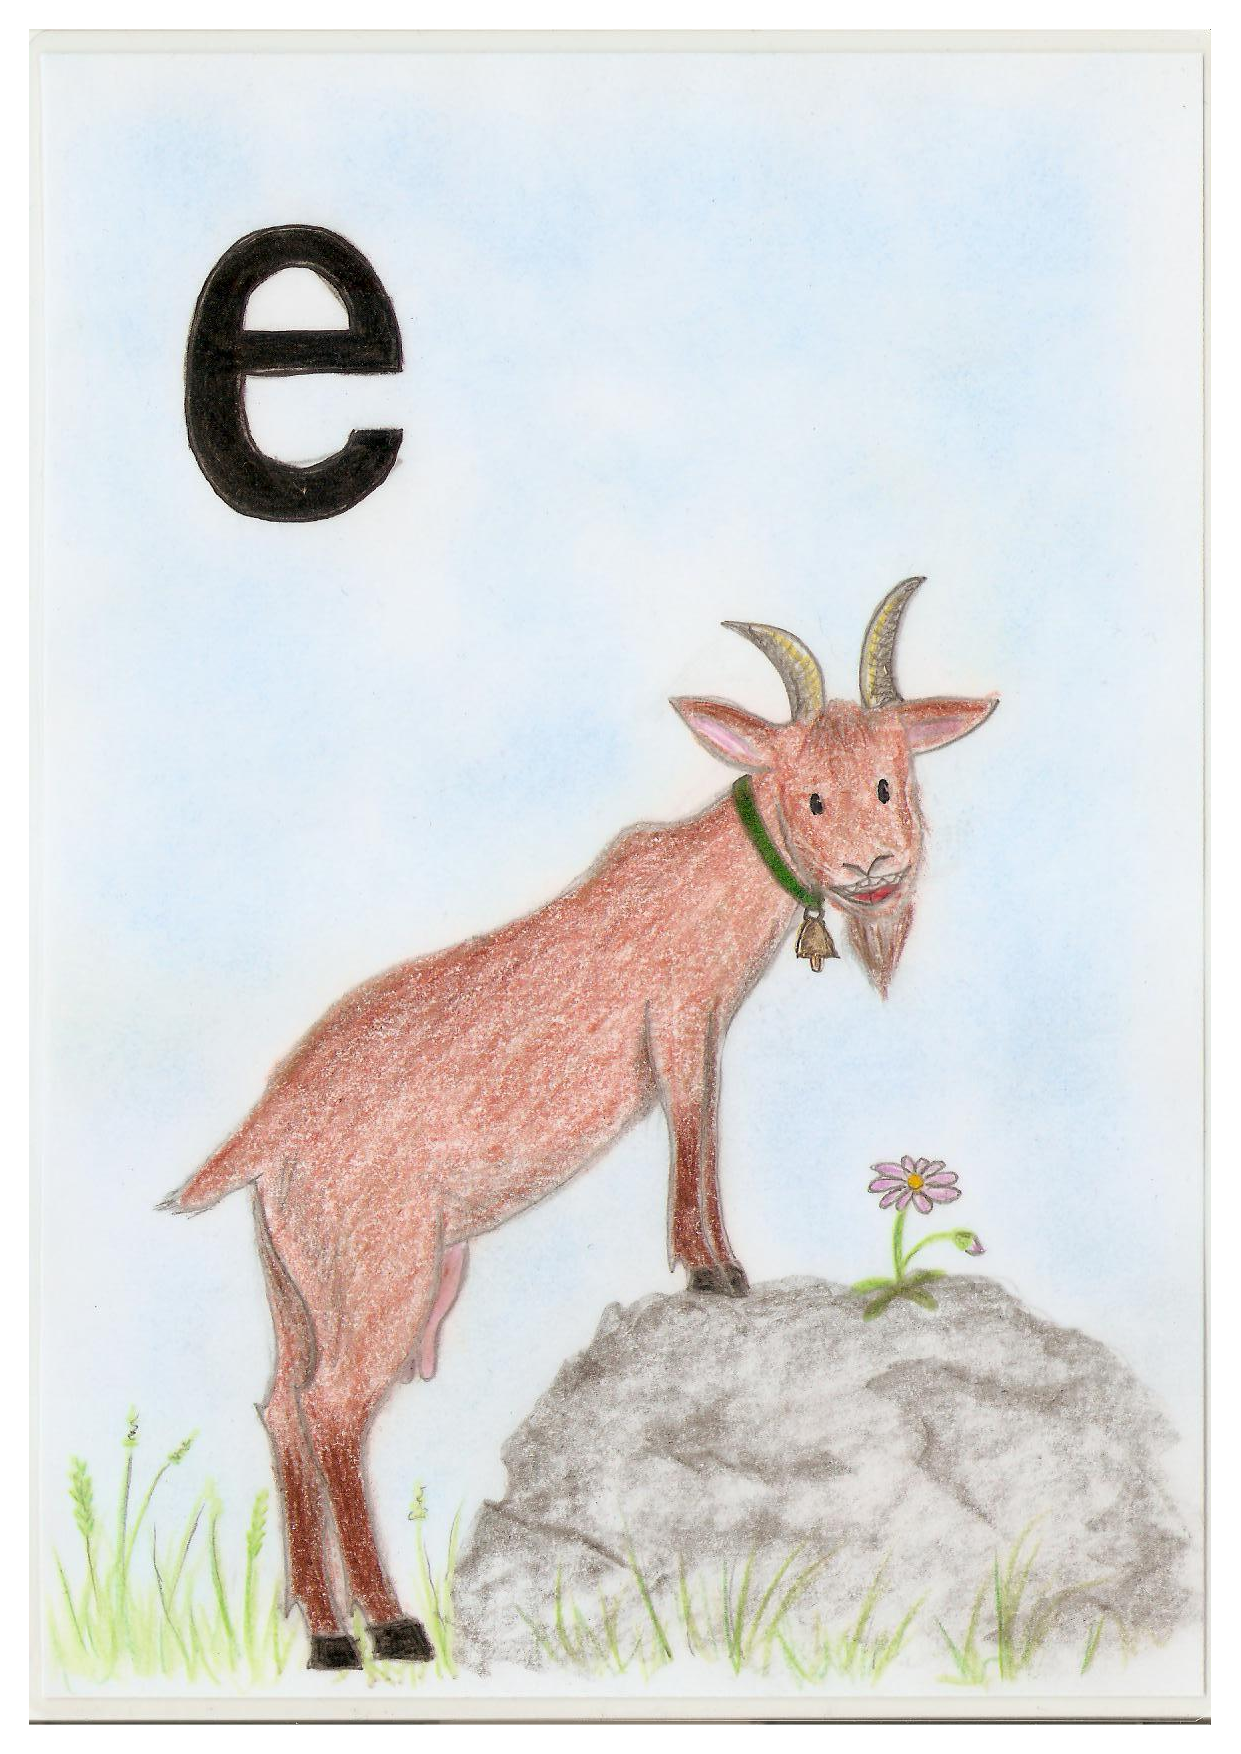
\includegraphics[width=.8\linewidth]{E}
  \caption{e}
\end{subfigure}
\begin{subfigure}{.33\textwidth}
  \centering
  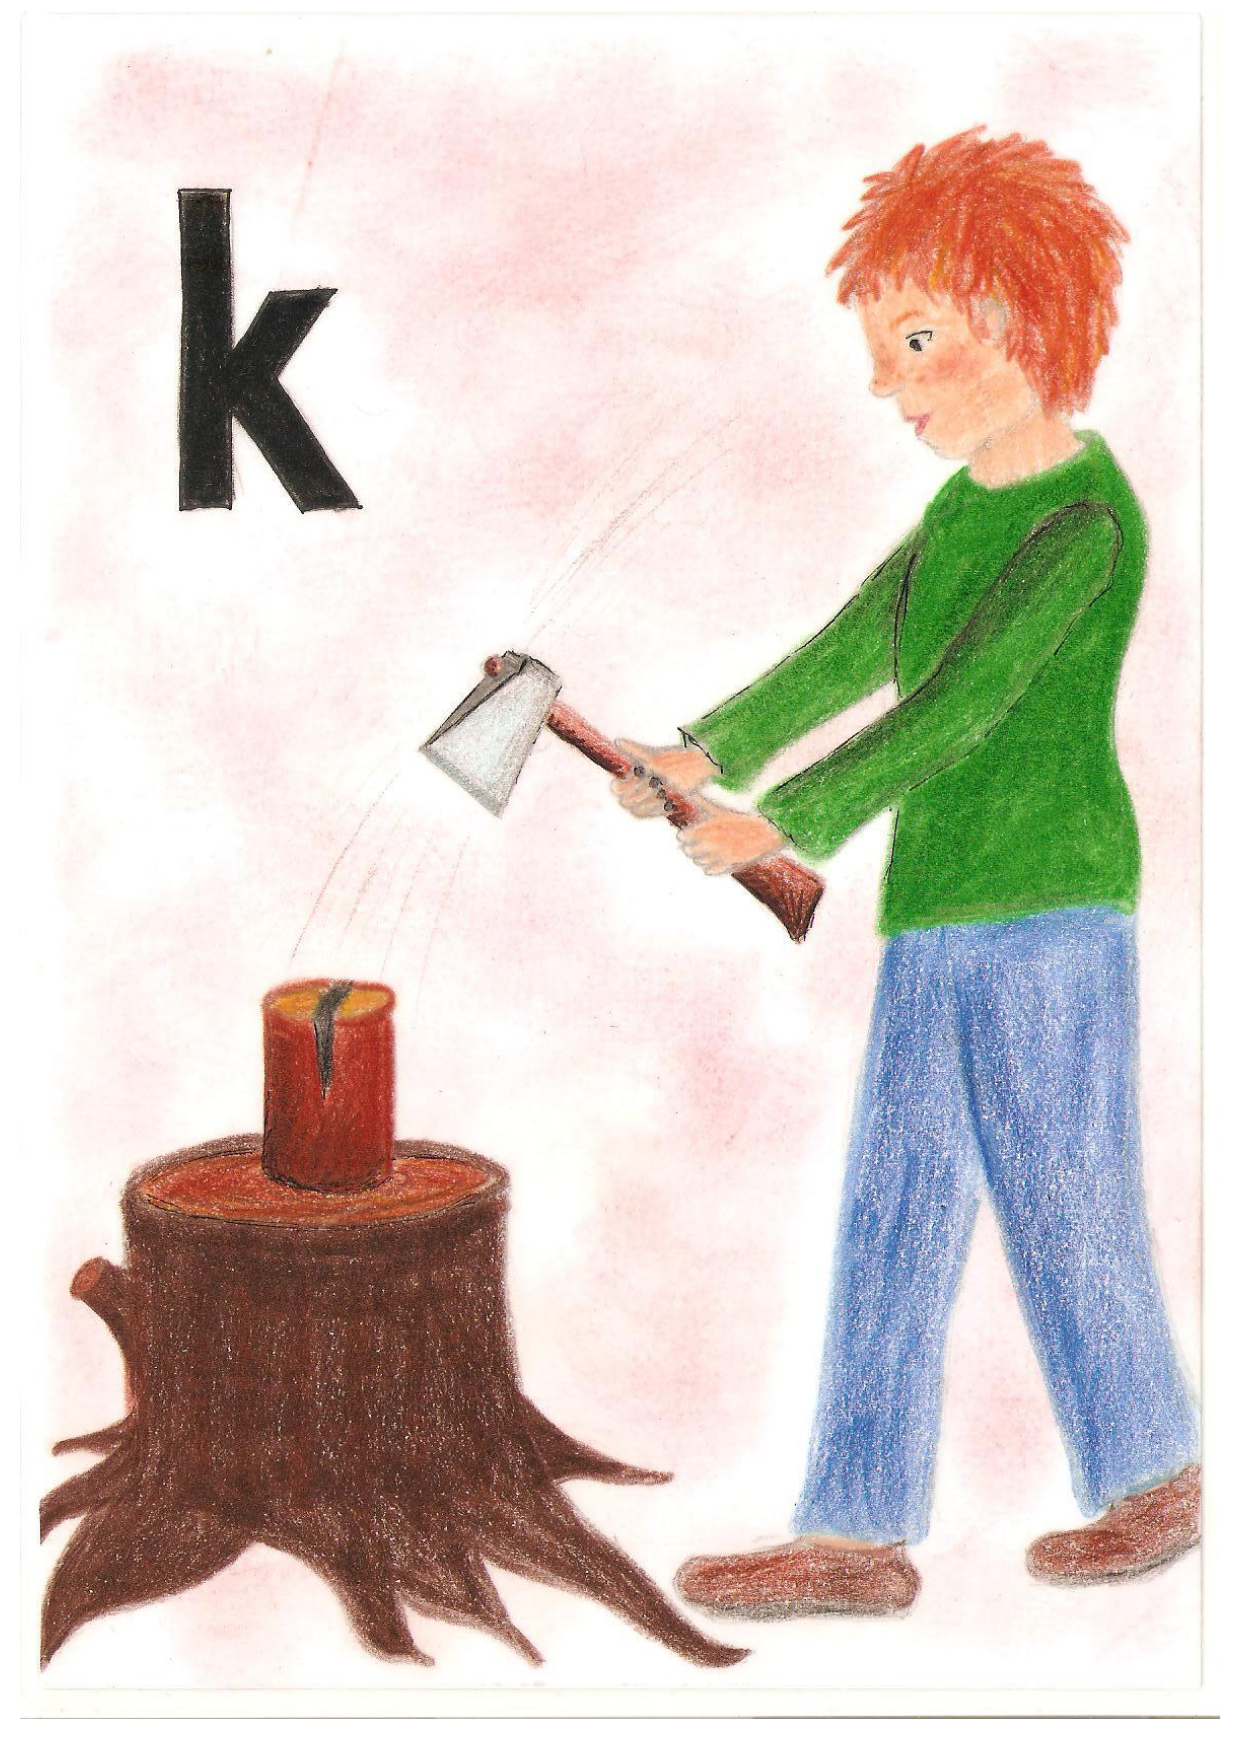
\includegraphics[width=.8\linewidth]{K}
  \caption{k}
\end{subfigure}
\caption{Examples of sound cards for children\cite{childImages}.}
\end{figure}



\subsubsection{Pre-defined word list (R18)}
While in the end, each patient is expected to be able to speak any word he wants to, not all words are equally suitable for supporting the therapy progress. Due to the nature of the language, German words in particular can be concatenated almost indefinitely and still make sense, which might be useful in general, but is highly unusable for therapy. Therefore, when generating new levels, the game takes words from a previously pre-defined word list which was selected with the therapist's help. Additionally, for each word present, there exist an own sound card if the game is played in child mode. As of now, the word list consists of 123 different words which cover all included target sounds as well as their possible positioning within the word (start, middle, or end) multiple times. This means that, for example, for the sound "d" there exist at least three words which start with "d", three which have "d"  in the middle and three that end with "d". This is to ensure sufficient randomness when creating new levels.

\subsubsection{Multiple voice recognition softwares (R29)}
While not initially planned, this feature proved to be necessary over the course of development. Since the game is meant to be played on the patient's laptop, all of its features have to work as intended regardless of the laptops' hardware (within reason of course). While for most features this does not pose an issue, the voice recognition software runs exactly into that problem. When testing the game on the therapist's laptop, the recognition system took too long to interpret voice input, thus leading to a slowed gameplay. To counter this issue, the usage of multiple voice recognition systems was proposed. Depending on the laptop's capabilities, the player can now choose between a \emph{fast} version, which is more suited for low-end devices, or a \emph{precise} version, which requires more computing power, but in return delivers better results. To realize this feature, two differently sized Whisper images were trained: one \textbf{tiny} and one \textbf{small}. The player can switch between these images within the main menu of the game.


\subsection{Use Case: Use additional help}
Depending on the patient's abilities and the difficulty of the current level, progress might be halted. While failing and repetition can be considered to be just a natural part of games as well as therapy, patients might become frustrated when no progress is achieved whatsoever. To counter this issue, one of two actions can be taken: Either the game or therapy is made easier or additional help is provided. Since the creation of levels and therapy progress are both tools of adapting difficulty that only the therapist can use, the second option is the only plausible course of action for developers. Thus, a total of three helping mechanisms have been implemented, which can all be found within a button-section in the game: A Skip-Button (R19), a Listen-Button (R20) and a Record-Button (R21).

\subsubsection{Skip-Button (R19)}
Whether the currently sought phrase is too difficult or the voice recognition software has issues correctly identifying it, patients could be stuck on one particular phrase for an extended time. Again, while constant practice is beneficial for therapy progress, it might become frustrating. Thus, in order to somewhat progress, a skip button will appear if the patient fails to correctly input the current phrase three times. Pressing this button skips the current phrase and proceeds to the next one. Note that skipping a phrase does not count it towards the accuracy-high-score metric and is entirely optional. After pressing the button, it disappears until the patient again fails for at least three times.

\subsubsection{Listen-Button (R20)}
When pressing the listen-button, the currently needed phrase is voiced to the player. This is yet another feature that was specifically added to aid young children, who cannot yet read, or patients who lost this ability after an accident. For most phrases, the button will play a previously recorded audio file in which the therapist herself voices the phrases. This supports the player by hearing the correct pronunciation of the phrase. In the case of randomly generated syllables within the syllabic levels, however, this was not an option as the amount of syllables generated were far too many for this case. Instead, for any such syllables, the phrase is voiced by using Google's text to speech engine. While functional, this approach has two notable drawbacks. First, the game has to have a working internet connection for this to work, otherwise the feature cannot be used. Secondly, Google's text-to-speech engine does not provide as good of a pronunciation than a real therapist does. Nonetheless, this solution still proves beneficial when compared to its absence.

\subsubsection{Record-Button (R21)}
The record-button introduces an alternative way to initiate voice input. Instead of pressing a predefined key, the patient can now use the mouse to start recording. This feature might not aid regarding pronunciation issues like the previous two buttons, but it makes the game more accessible since by introducing this button, the usage of a keyboard for the game becomes obsolete. While currently not planned, this makes porting the game to mobile devices easier, which in turn increases accessibility.


\begin{figure}
\begin{center}
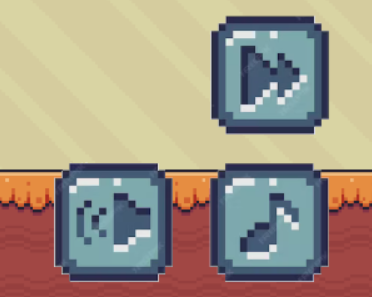
\includegraphics[scale=0.4]{LE_Help}
\end{center}
\caption{The help-buttons present within a level. Top Right: Skip jump, bottom left: Start recording and bottom right: Listen to phrase.}
\end{figure}
\subsection{Use Case: View High-Scores}
While not essential to the game, introducing a High-Score system is beneficial regarding player motivation as well as progress tracking. For these two reasons, two types of High-Scores have been included: High-Score-time (R22) and High-Score-accuracy (R23). Highscore-time simply measures the time needed for the player to finish the current level, with lower values being preferred. In contrast, High-Score-accuracy measures how accurate the player was during the level in the following way. If the player manages to correctly pronounce a phrase on the first try, he gets a point. This is, however, only true for the first try, i.e., when pronouncing the phrase correctly on the second or third attempt, no point is given. At the end of the level, the accuracy-score is calculated by dividing the number of points gathered by the number of phrases played. The result is a value between 0 and 1, which is then displayed as a percentage. This value is also used for unlocking new levels (i.e., only with an accuracy of x\% or higher it is possible to play the next level) and can be changed via the main menu.

\begin{figure}
\begin{center}
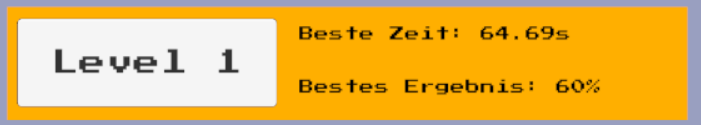
\includegraphics[scale=0.5]{LE_Scores}
\end{center}
\caption{The time- and accuracy high scores for one level.}
\end{figure}

\subsection{Use Case: Change Settings}
At any given time, the game is customizable to some degree by either the patient or the therapist. Such customizations include:
\begin{itemize}
\item \textbf{Toggle stress component (R11)}: Toggles whether there should be lava rising from the bottom in each level. This feature is disabled by default and intends to provide an additional challenge to more experienced players.

\item \textbf{Configure audio volume (R15)}: Players can toggle the audio volume of the game on a scale of 0 (muted) to 100 (maximum volume). By default, the audio volume is set to 100. This setting affects all audio within the game, meaning both animation sounds and background music intensity can be altered.

\item \textbf{Enable child mode (R17)}: Toggles whether children-specific sound cards or lip movement images are displayed within the level. As the collaborating therapist mostly works with children, this setting is enabled by default.

\item \textbf{Set accuracy thresholds (R23)}: New levels within the game are only unlocked once the player reaches a certain accuracy-High-Score on the previous level. This threshold can again be configured within the settings menu and can be selected from 0\% to 100\% in increments of 10. Per default, an accuracy threshold of 80\% is selected.

\item \textbf{Switch voice recognition model (R30)}: Depending on the player's end device, the most precise model might be too computational expensive. Thus, players can  switch between a \emph{fast} and \emph{precise} recognition mode. Per default, the fast mode is selected.
\end{itemize}
All these settings are accessible from the main menu.

\begin{figure}
\begin{center}
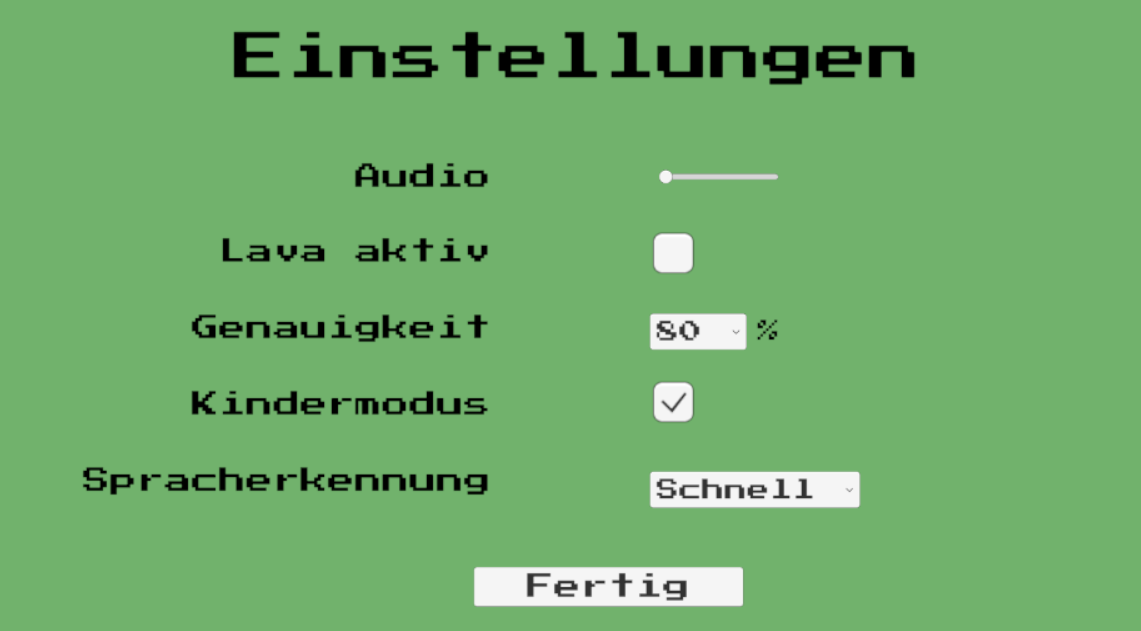
\includegraphics[scale=0.4]{LE_Settings}
\end{center}
\caption{The settings screen for the game.}
\end{figure}

\subsection{Use Case: Navigate Game} 
Since having all information displayed at once is too convoluted, it makes sense to split up the game into multiple scenes. These scenes mainly consist of the start screen (\textbf{R7}), a level overview scene (\textbf{R8}) and an info scene (\textbf{R14}).

\subsubsection{Start screen (R7)}
The start screen is the welcoming page when initializing the game. From here, both patient and therapist can navigate further to the game settings, the export menu, the info screen or start the game. Regarding navigation, it thus poses as the most central component within the game.

\subsubsection{Level overview screen (R8)}
The level overview scene shows which categories the patient can play. These categories were ideally predefined by the therapist beforehand, but if necessary can be generated by the patient himself using the button at the bottom. Selecting a category then guides the player to the level list for this category, with unlocked levels being enabled and others disabled. For each level, the current High-Scores are also displayed. Using the back-button in the top left corner returns the player to the start screen.

\subsubsection{Info screen (R14)}
While not necessary regarding gameplay, an info screen can be accessed via the start screen. This info screen aims to highlight the game's intended usage as well as mentions and thanks all parties involved in creating the game, including therapists and asset creators.

\begin{figure}
\begin{center}
\begin{subfigure}{.9\textwidth}
  \centering
  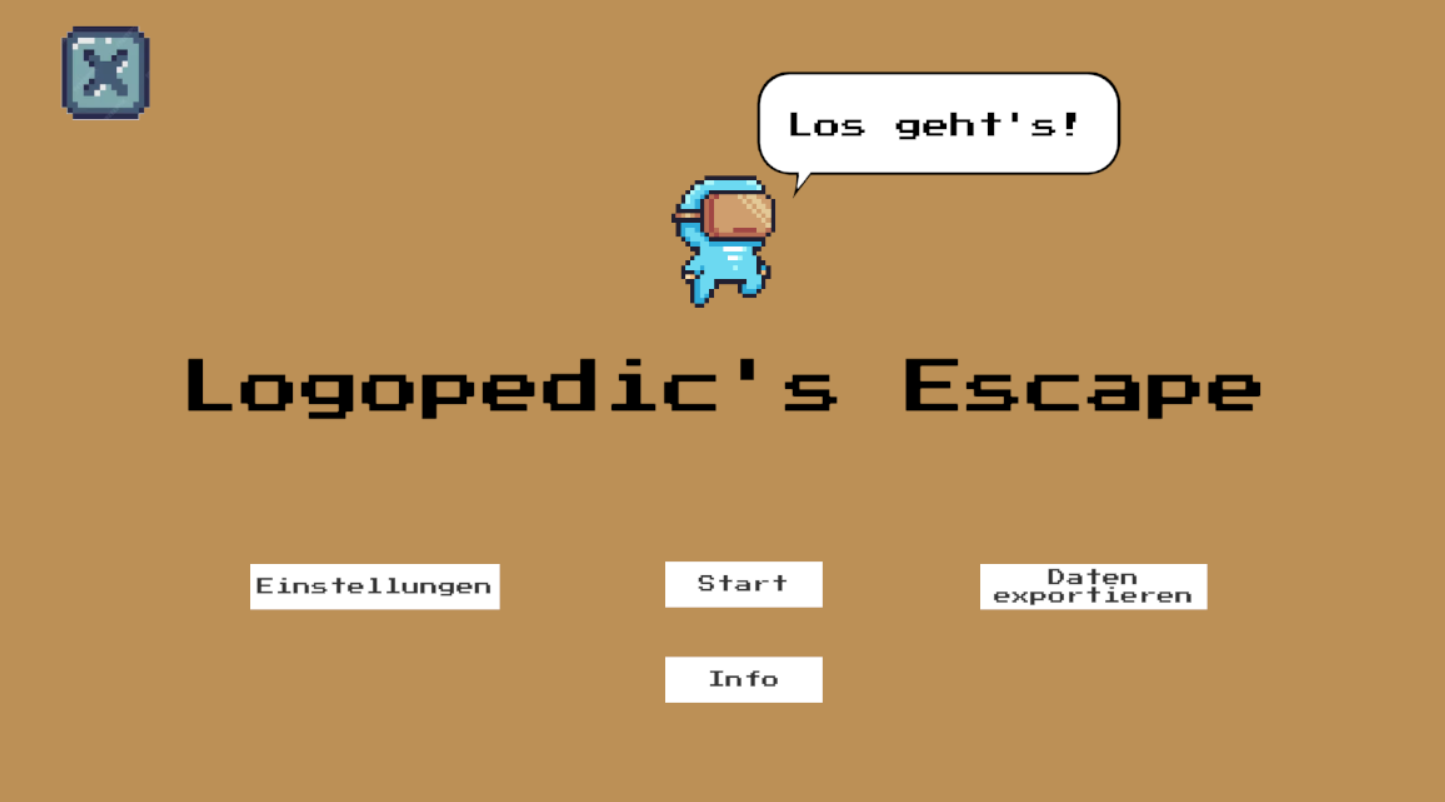
\includegraphics[width=.8\linewidth]{LE_Start}
  \caption{Start screen}
\end{subfigure}
\begin{subfigure}{.9\textwidth}
  \centering
  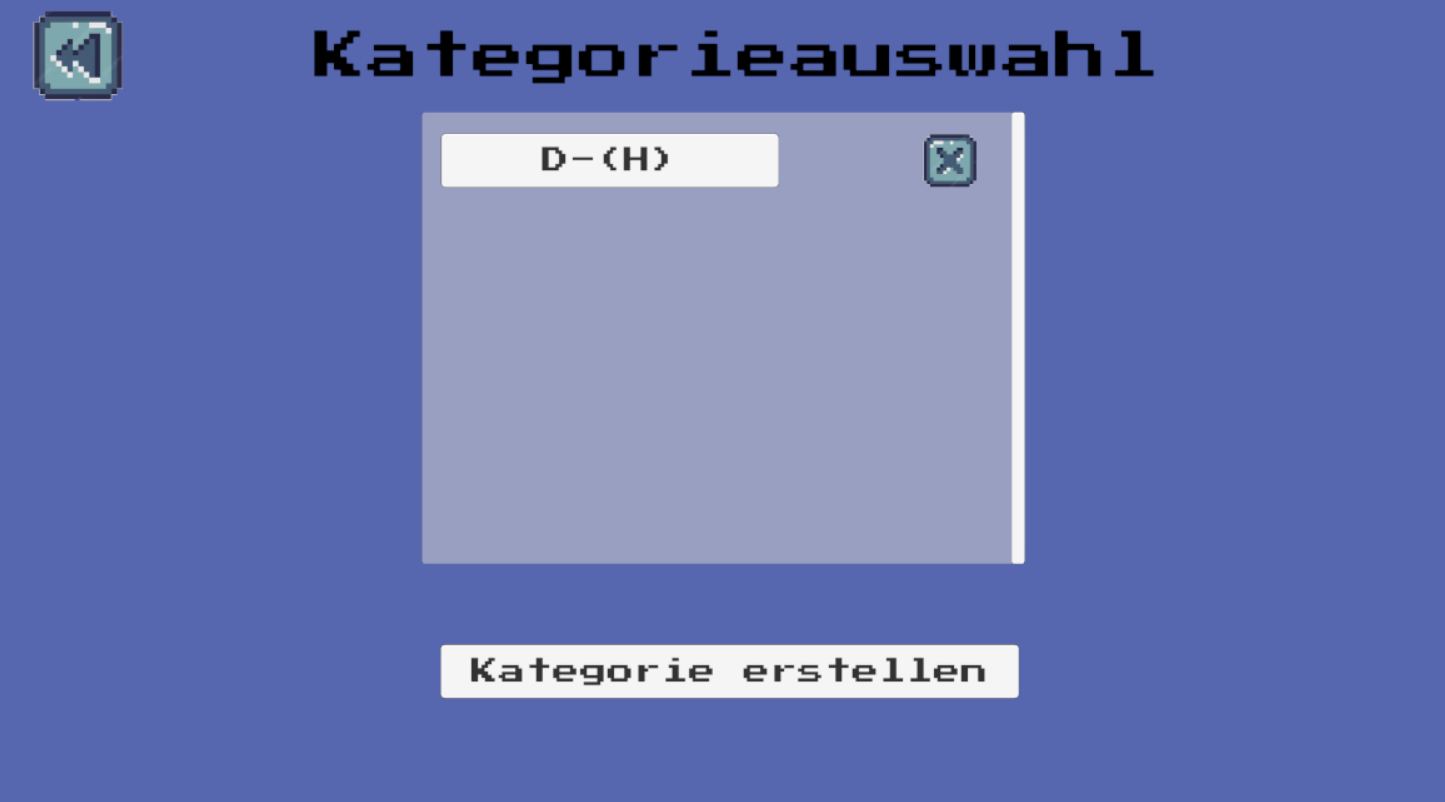
\includegraphics[width=.8\linewidth]{LE_LevelOverview}
  \caption{Level overview}
\end{subfigure}
\begin{subfigure}{.9\textwidth}
  \centering
  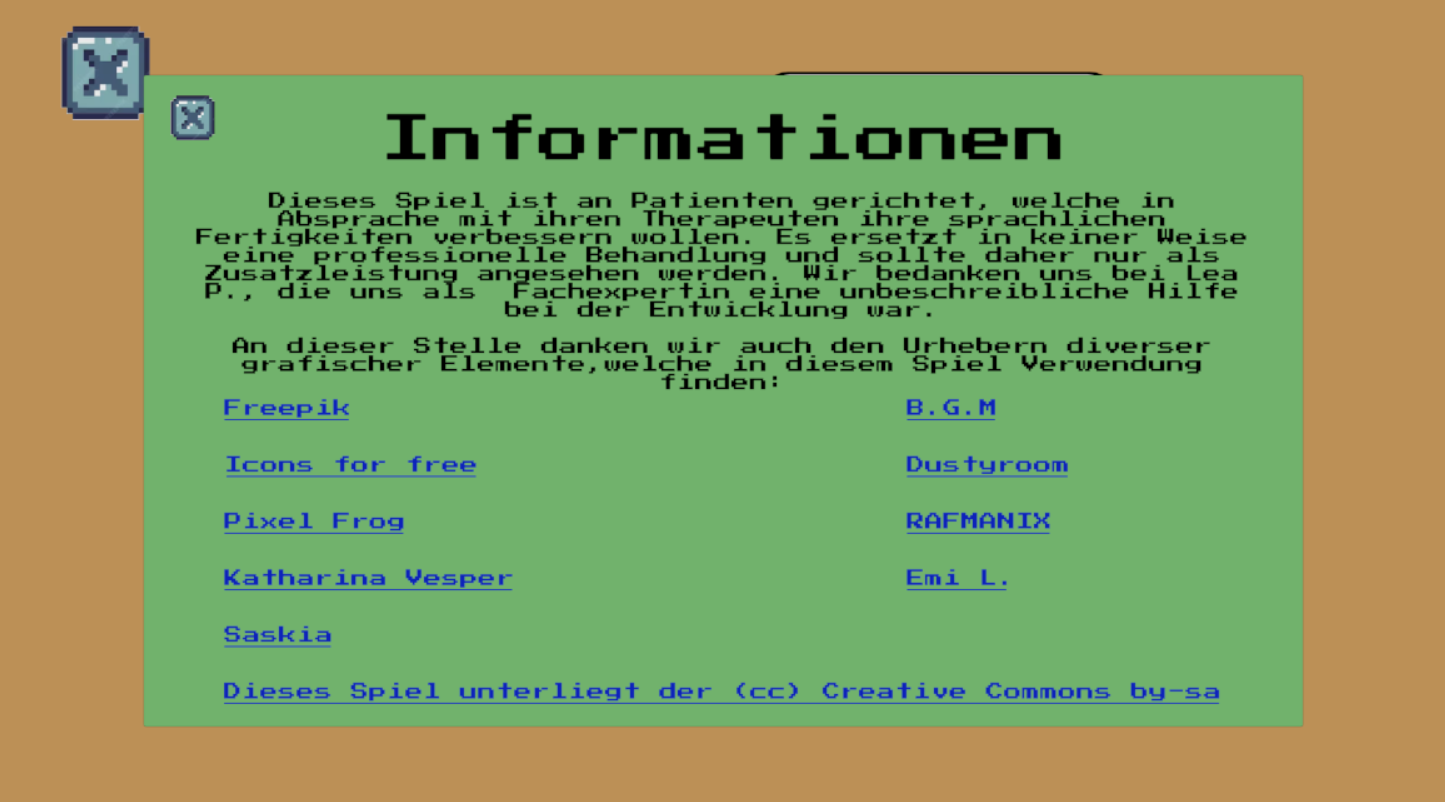
\includegraphics[width=.8\linewidth]{LE_Info}
  \caption{Info screen}
\end{subfigure}
\caption{Navigational screens of the game.}
\end{center}
\end{figure}

\subsection{Use Case: Edit category}
Before instructing the patient to play the game, the therapist first has to create at least one level category. A category is synonymous to a set of levels which all aim to practice one sound in different environments (i.e., the sound "d" shall be practiced on the phonetic, syllabic and word stage). The therapist can define which sound is to be practiced, as well as whether and how many distracting sounds are present within the levels. While not inherently necessary, distracting sounds aim to further emphasize on the clear distinction between different sounds and thus are a helpful tool within therapy \cite{proestler2023}. This Use-Case consists of three requirements: category creation (R25), category customization (R26) and category deletion (R28), all of which are quite self-explanatory and thus will not be elaborated on further.

\begin{figure}
  \centering
  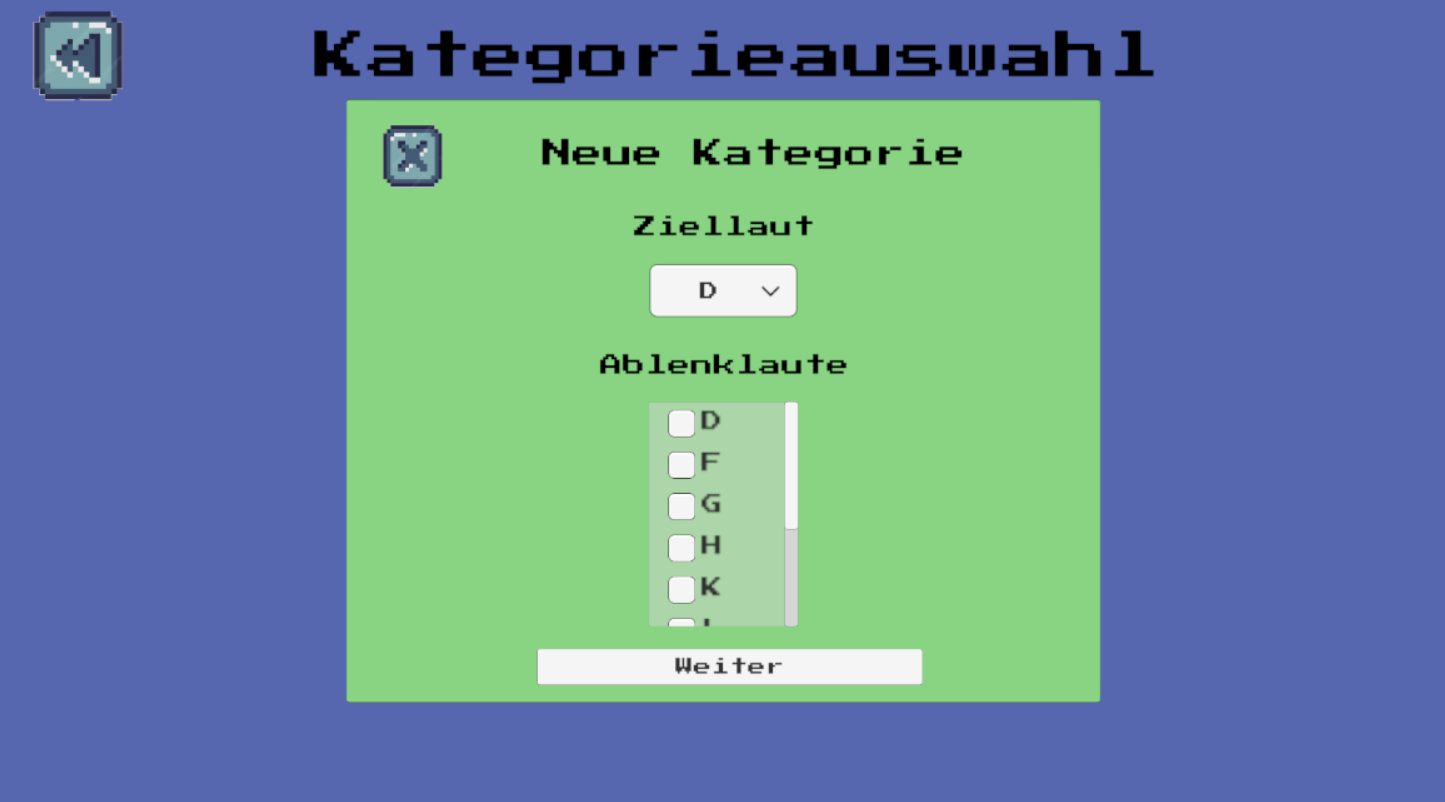
\includegraphics[width=.8\linewidth]{LE_CategoryEditor}
  \caption{Category edit Screen.}
\end{figure}

\subsection{Use Case: Edit level}
Having defined the category's parameters, the therapist can then define each level regarding the following parameters:
\begin{itemize}
\item \textbf{Include level}: Determines whether the level is to be included within the category. This is useful if the therapist wants to create a category which has less than the default number of levels (14 as of now). As of now, the default number of levels stems from a permutation of possible difficulty increases. The main factors that influence difficulty are the level type (sound, syllable, word), the positioning of the target sound within phrases (start, middle or end; not applicable for sound stage levels) and whether distracting sounds should be included.
\item \textbf{Therapy stage}: Defines which therapy stage (phonetic, syllabic or word) the current level includes. Usually, the first levels are based on earlier stages than later ones, but again, the therapist can change this if necessary.
\item \textbf{Sound placement}: Defines where within the phrase the exercised sound is located. Possible placements are at the start, in the middle or at the end. This setting is not available for phonetic stage levels. Additionally, depending on the target sound of the category, not all options might be available. For example, since the sound of 'r' is never pronounced at the end of words in German (meaning that if a german word ends in 'r' it is silent), if 'r' has been selected as the target sound, the option to generate levels with phrases that end in 'r' is not available. This feature is meant to aid therapists in preventing customization mistakes.
\item \textbf{Include distracting sounds}: If selected, the level will alternate between phrases that include the target sound previously defined within category creation, and ones which include one of the selected distracting sounds.
\end{itemize}
Note that default level settings are present, i.e., the therapist does not have to change anything to be able to create the levels, but can if he so desires. The default settings are ordered by degree of difficulty, meaning that easier settings come before more difficult ones, though the perception of "easy" and "difficult" might differ from patient to patient.

\begin{figure}
  \centering
  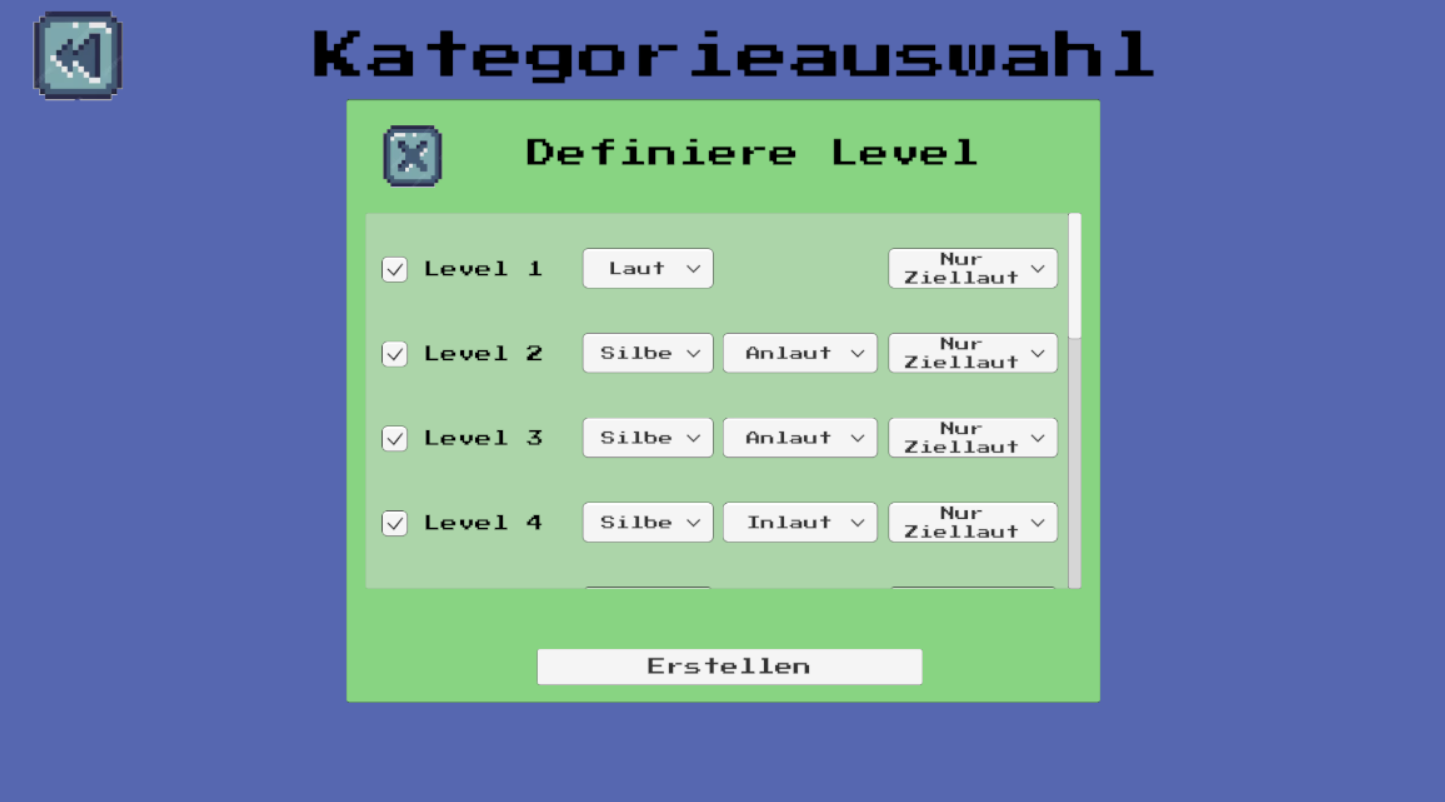
\includegraphics[width=.8\linewidth]{LE_LevelEditor}
  \caption{Level edit screen}
\end{figure}


\subsection{Use Case: Review patient performance}
In order to measure progress, the therapist must employ some kind of metric after which the patient's performance can be judged. The requirements regarding this Use-Case are the Data Log (R16) and the accuracy- and time High-Scores (R22 and R23 respectively).
\subsubsection{Data Log}
This requirement is quite synonymous for \emph{RQ2}. During the first interview with the therapist, it was discovered that there currently does not exist a single standardized progress tracking tool or mechanism for speech therapy that was used by most of or all therapist. Instead, each therapist has his own way of tracking patient progress specifically tailored for their process. However, both the author and the therapist could identify four different progression metrics (AST, MCM, Level  completion time, Level accuracy) that can be useful for measuring therapy progress. While logging these four metrics occurs while the patient plays the game, the therapist could additionally export all this data to an external CSV-file, which can then be later on included in the therapist's Excel-files.

\begin{figure}
  \centering
  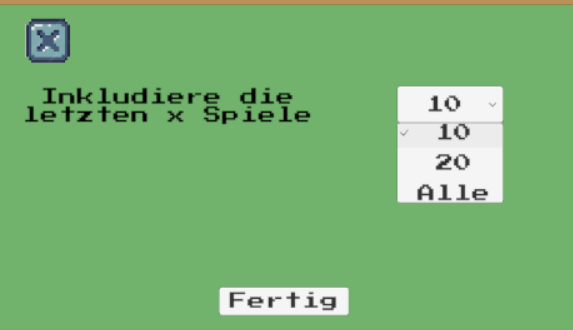
\includegraphics[width=.6\linewidth]{LE_Export}
  \caption{Data Export options.}
\end{figure}

\section{Game Architecture}
\begin{figure}
  \centering
  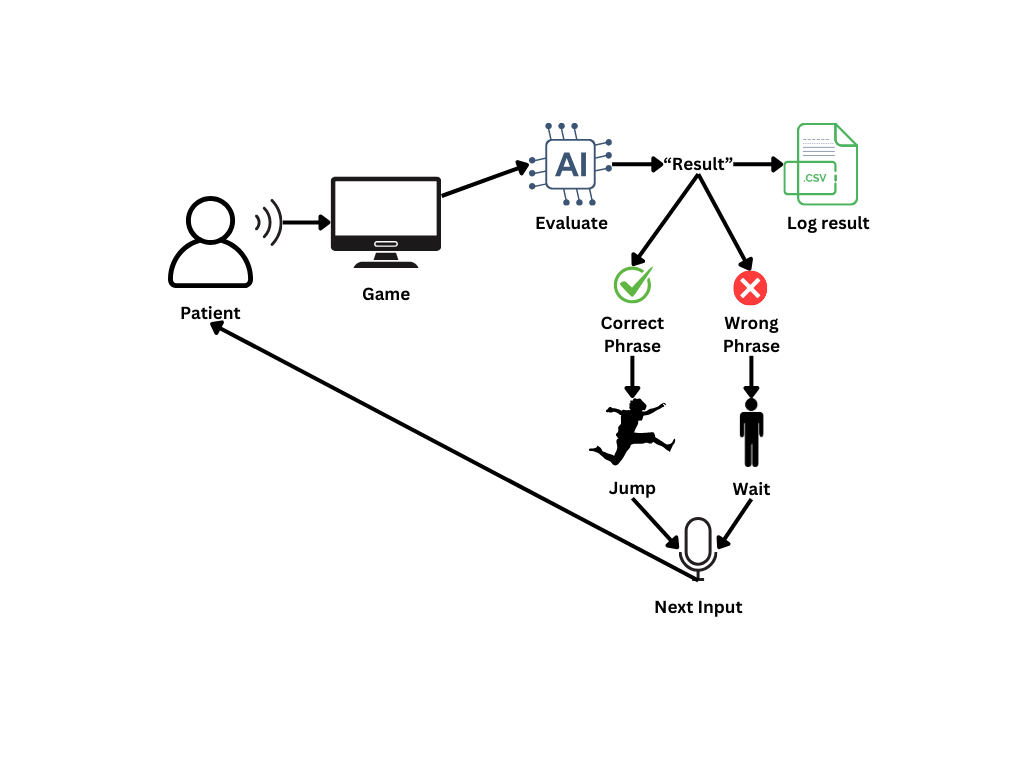
\includegraphics[width=.9\linewidth]{GameplayLoop}
  \caption{The game's main gameplay loop.}
  \label{fig:architecture}
\end{figure}
Depending on how much into detail one wants to go, elaborating on the architecture of the game is more or less complex. This section aims to both give a brief summary on the high-level architecture of the game's main gameplay process as well as provide more in-depth information later on. \\
Starting with the rough architecture, Figure \ref{fig:architecture} depicts all core components used when playing the game. First, the patient provides voice data by attempting to correctly voice the current phrase. This voice data is then evaluated by the previously trained voice recognition model and thus transformed into text. The text is immediately written into an additional data file in order for the therapist to review the patient's performance later on (logging capability). Depending on whether the phrase is correct or not, the avatar either jumps to the next platform or remains vacant. The game then awaits further input from the patient, starting the whole process anew. \\


Looking into the game itself in more detail, additional information can provided. The requirements mentioned in Section \ref{sec:Features} were implemented within the Serious Game using the Unity Editor (v. 2022.3.9f1). Additional functionality was programmed using C\# scripts, which can be easily integrated within Unity as \emph{components}. Generally speaking, the Unity game architecture consists of three big hierarchies. \emph{Scenes} describe whole in-game scenarios like single levels or menu screens. Each Scene is filled with multiple \emph{GameObjects}. Typical GameObjects include Cameras (i.e., viewpoints of the scene), the player avatar, platforms or UI elements. Last but not least, each GameObject consists of multiple \emph{Components} which describe the GameObject's behaviour. For example, the player avatar usually needs some kind of RigidBody and Collider component in order to detect collisions with other GameObjects. Many of these components are readily available by Unity, but custom components called \emph{Scripts} can also be added. \\

For this work in particular, free in-game assets from the Unity Asset Store \cite{unityStore} have been used. Table \ref{tbl:unityAssets} provides a brief summary. Similarly, Table \ref{tbl:unityLibraries} lists all additional libraries within the project.

\begin{longtable}[h]{|c|c|}
\hline
\textbf{Name} & \textbf{Description} \\  \hline
2D Atlas Speechbubbles  Alphabet Numbers \cite{assetSpeechBubble} & Provides speech bubble asset \\ \hline
ArcadeGameBGM\# 17 \cite{assetArcadeBGM} & Provides background  \\ \hline 
Basic Icons by Kandles \cite{assetBasicIcons}& Provides Menu buttons \\ \hline
CasualGameBGM05 \cite{assetCasualBGM}& Provides background  music \\ \hline
CasualGameSounds \cite{assetCasualGameSounds}& Provides animation sounds \\ \hline
PressStart2Play \cite{assetPressStart}& Font used in the game \\ \hline
Pixel Adventure 1 \cite{assetPixelAdventure1}& Provides avatar assets \\ \hline
Pixel Adventure 2 \cite{assetPixelAdventure1}& Provides background assets \\ \hline


\caption{Used assets for the game.}
\label{tbl:unityAssets}
\end{longtable}


\begin{longtable}[h]{|c|c|c|}
\hline
\textbf{Name} &  \textbf{Description}  & \textbf{Version}\\  \hline
Whisper & Adapts Whisper image into the game & 1.0.0 \\ \hline
JetBrains Rider Editor & Integration for developing editor & 3.0.24 \\ \hline
Shader Graph & Used for animating lava & 14.0.8 \\ \hline
TextMeshPro & Used for displaying and stylizing UI text & 3.0.7 \\ \hline


\caption{Used additional assets for the game.}
\label{tbl:unityLibraries}
\end{longtable}

\begin{figure}
  \centering
  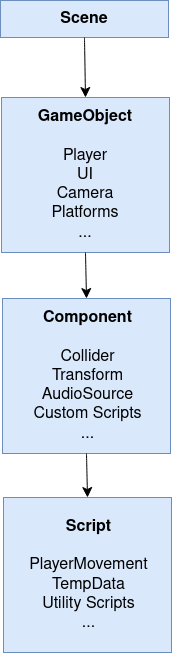
\includegraphics[width=.2\linewidth]{Unity_Structure}
  \caption{General structure of Unity games.}
\end{figure}
The game prototype also implements custom Scripts to cover certain features needed. Due to better readability and possible re-usability, those Scripts are separated regarding their functionality. Additionally, the scripts used can be classified by where within the game they are used. Over the course of this thesis, six categories were identified: \textbf{Avatar, Settings, Level, Category, Logging } and \textbf{General}. Table \ref{tbl:gameScripts} briefly elaborates on all scripts implemented.

\begin{longtable}[h]{|p{.20\textwidth}|p{.70\textwidth}|}
\hline
\textbf{Name} &  \textbf{Description} \\  \hline
\multicolumn{2}{|c|}{\textbf{Avatar Scripts}} \\ \hline
CameraController &  Dynamically sets the camera to always focus on the avatar, even during movement. \\ \hline
PlayerLife & Evaluates whether the avatar is alive or not. This toggles the "Game Over" screen. \\ \hline
PlayerMovement & Handles avatar animation for different movements (i.e., running, falling, staying idle). \\ \hline
SpeechToText & Translates recorded audio into text using the provided Whisper model. If the text matches the needed phrase, the jump to the next platform is initiated. \\ \hline
NextJumpModel & A model class that defines a jump's characteristics (i.e., key-phrase and x- and y-velocity). \\ \hline
\multicolumn{2}{|c|}{\textbf{Level Scripts}} \\ \hline
CheckIfNextLevel- Exists & Checks whether the current level has a successor. This is needed in order to toggle the "Next Level" button visibility in the finish-screen. \\ \hline
Finish & Toggles finish-screen visibility as well as initiate some logging processes. \\ \hline
ImageSwap & Swaps mouth gesture images or sound cards whenever the player succeeds on the current jump. \\ \hline
LavaHeight & Responsible for displaying the current lava height in the UI. \\ \hline
LavaMovement & Continually raises the lava's current height. \\ \hline
LevelTimer & Displays the current level's time in the UI. \\ \hline
LevelModel & A model class that defines the level's characteristics (i.e., phrase placement and distracting sound inclusion). It is used during the level initialization process. \\ \hline
PauseGame & Pauses the level. This includes freezing all player and lava movement as well as stopping the level timer. \\ \hline
PlayerHeight & Displays the current height of the player in the UI. \\ \hline
ReadJumpModels & Reads in all NextJumpModels for the level from an external .csv file. Used during level initialization. \\ \hline
RestartLevel & Restarts the current level. \\ \hline
SetPhrases & Sets the phrase labels for each jump within the level. Used after ReadJumpModels during level initialization. \\ \hline
SkipJump & Executes the next jump without having to voice the correct phrase. This script is used for the skip-button. \\ \hline
TipsVisibility & Toggles whether mouth gesture pictures or sound cards are visible. In child mode, sound cards are  always visible. \\ \hline
ToggleHint & Toggles the first hint's ("Press M to record") visibility. \\ \hline
ToggleLevel-SettingsVisibility & Enables/Disables the level settings screen. \\ \hline
TogglePhrases & Toggles phrase visibility so that only the phrase of the current jump is visible. \\ \hline
ToggleRecording & Toggles recording state. This Script is used when voice recording using the UI-button. \\ \hline
TextToSpeech & Implements the functionality behind the listen-button. \\ \hline
\multicolumn{2}{|c|}{\textbf{Settings Scripts}} \\ \hline
ChangeAudio-Volume & Changes in-game audio volume and saves it as a preference. \\ \hline
ChangeLavaPref & Used to toggle the inclusion of lava within the levels. \\ \hline
SaveAccuracyPref & Saves the accuracy score required for progressing to the next level. \\ \hline
SaveSpeech-RecognitionPref & Saves which voice recognition model (\emph{fast} or \emph{precise}) should be used within the game. \\ \hline
ToggleSettings-Visibility & Displays or hides the settings screen. \\ \hline
\multicolumn{2}{|c|}{\textbf{Categories Scripts}} \\ \hline
CreateNew-Category & Creates a new category with the given settings. This includes creating a custom category folder in the \emph{StreamingAssets} folder of Unity, as well as generating a custom level file for each level which contains information such as key-phrases and jump-values for each level. \\ \hline
DeleteCategory & Deletes a given category. This includes deleting the category folder within \emph{StreamingAssets} as well as removing all related highscores within the game. \\ \hline
LoadCategories & Loads all available categories from the \emph{StreamingAssets folder}. Used for displaying available categories to the player. \\ \hline
LoadLevels & Loads all available levels and their highscores for a category. This is again used to display the levels to the player. \\ \hline
SaveCurrent-Category & Saves the current category and level selection into a temporary class. Doing this allows data to persist over multiple scenes and thus can be used to influence the level selection screen and the level themselves. \\ \hline
\multicolumn{2}{|c|}{\textbf{Logging Scripts}} \\ \hline
ExportLogs & Allows the player to export a log-file in .csv format from the game. As of now, the location of the export is fixed due to an unresolved issue. \\ \hline
LevelLogger & This class is responsible for logging player activity during playtime. Metrics such as MCM and AST are logged for every jump, while accuracy- and time-highscores are saved only at the end of each level. \\ \hline
\multicolumn{2}{|c|}{\textbf{General Scripts}} \\ \hline
GoToScene & Adds a visual transition component when switching scenes. \\ \hline
LinkHandlerFor-TMPText & Allows embedding hyperlinks within texts in the game. \\ \hline
QuitGame & Exits the game. \\ \hline
TempData & A static class which is used to store state-data while playing the game. It is used to correctly display available levels or to load correct level files. This class is newly initialized whenever the game is started, meaning it cannot be used to store persistent data. \\ \hline
ToggleButton-Image & Allows images for buttons to be easily replaced when pressing them. \\ \hline


\caption{The Serious Game's scripts.}
\label{tbl:gameScripts}
\end{longtable}

\begin{comment}
The Avatar Scripts handle custom functionality for the player avatar and comprise of the following Scripts:
\begin{itemize}
\item \textbf{CameraController}: Dynamically sets the camera to always focus on the avatar, even during movement.
\item \textbf{PlayerLife}: Evaluates whether the avatar is alive or not. This toggles the "Game Over" screen.
\item \textbf{PlayerMovement}: Handles avatar animation for different movements (i.e., running, falling, staying idle).
\item \textbf{SpeechBubble}: Toggles the visibility and content of the speech bubble that appears when the player issues a voice command.
\item \textbf{SpeechToText}: Translates recorded audio into text using the provided Whisper model. If the text matches the needed phrase, the jump to the next platform is initiated.
\item \textbf{NextJumpModel}: A model class that defines a jump's characteristics (i.e., key-phrase and x- and y-velocity).
\end{itemize}


The above scripts as well as some of Unity's pre-defined Components allow for the avatar to behave as required. Next, the Level scripts define how the avatar's surrounding behaves. The following scripts influence the Level environment:
\begin{itemize}
\item \textbf{CheckIfNextLevelExists}: Checks whether the current level has a successor. This is needed in order to toggle the "Next Level" button visibility in the finish-screen.
\item \textbf{Finish}: Toggles finish-screen visibility as well as initiate some logging processes.
\item \textbf{ImageSwap}: Swaps mouth gesture images or sound cards whenever the player succeeds on the current jump.
\item \textbf{LavaHeight}: Responsible for displaying the current lava height in the UI.
\item \textbf{LavaMovement}: Continually raises the lava's current height.
\item \textbf{LevelTimer}: Displays the current level's time in the UI.
\item \textbf{LevelModel}: A model class that defines the level's characteristics (i.e., phrase placement and distracting sound inclusion). It is used during the level initialization process.
\item \textbf{PauseGame}: Pauses the level. This includes freezing all player and lava movement as well as stopping the level timer.
\item \textbf{PlayerHeight}: Displays the current height of the player in the UI.
\item \textbf{ReadJumpModels}: Reads in all NextJumpModels for the level from an external .csv file. Used during level initialization.
\item \textbf{RestartLevel}: Restarts the current level.
\item \textbf{SetPhrases}: Sets the phrase labels for each jump within the level. Used after ReadJumpModels during level initalization.
\item \textbf{SkipJump}: Executes the next jump without having to voice the correct phrase. This Script is used for the skip-button.
\item \textbf{TipsVisibility}: Toggles whether mouth gesture pictures or sound cards are visible. In child mode, sound cards are always visible.
\item \textbf{ToggleHint}: Toggles the first hint's ("Press M to record") visibility.
\item \textbf{ToggleLevelSettingsVisibility}: Enables/Disables the level settings screen.
\item \textbf{TogglePhrases}: Toggles phrase visibility so that only the phrase of the current jump is visible.
\item \textbf{ToggleRecording}: Toggles recording state. This Script is used when voice recording using the UI-button.
\item \textbf{TextToSpeech}: Implements the functionality behind the listen-button.
\end{itemize}

Next, the settings-screen employs the following additional scripts:
\begin{itemize}
 \item \textbf{ChangeAudioVolume}: Changes in-game audio volume and saves it as a preference.
 \item \textbf{ChangeLavaPref}: Used to toggle the inclusion of lava within the levels.
 \item \textbf{SaveAccuracyPref}: Saves the accuracy score required for progressing to the next level.
 \item \textbf{SaveSpeechRecognitionPref}: Saves which voice recognition model (\emph{fast} or \emph{precise}) should be used within the game.
 \item \textbf{ToggleSettingsVisibility}: Displays or hides the settings screen.
\end{itemize}

For creating custom categories, additional scripts are needed as well:
\begin{itemize}
\item \textbf{CreateNewCategory}: Creates a new category with the given settings. This includes creating a custom category folder in the \emph{StreamingAssets} folder of Unity, as well as generating a custom level file for each level which contains information such as key-phrases and jump-values for each level.
\item \textbf{DeleteCategory}: Deletes a given category. This includes deleting the category folder within \emph{StreamingAssets} as well as removing all related highscores within the game.
\item \textbf{LoadCategories}: Loads all available categories from the \emph{StreamingAssets} folder. Used for displaying available categories to the player.
\item \textbf{LoadLevels}: Loads all available levels and their highscores for a category. This is again used to display the levels to the player.
\item \textbf{SaveCurrentCategory}: Saves the current category and level selection into a temporary class. Doing this allows data to persist over multiple scenes and thus can be used to influence the level selection screen and the levels themselves.  
\end{itemize}

For logging the player's activity, two additional scripts were implemented:
\begin{itemize}
\item \textbf{ExportLogs}: Allows the player to export a log-file in .csv format from the game. As of now, the location of the export is fixed due to an unresolved issue.
\item \textbf{LevelLogger}: This class is responsible for logging player activity during playtime. Metrics such as MCM and AST are logged for every jump, while accuracy- and time-highscores are saved only at the end of each level.
\end{itemize}

Last but not least, some scripts were used globally and thus persist in multiple scenarios:
\begin{itemize}
\item \textbf{GoToScene}: Adds a visual transition component when switching scenes.
\item \textbf{LinkHandlerForTMPText}: Allows embedding hyperlinks within texts in the game.
\item \textbf{QuitGame}: Exits the game.
\item \textbf{TempData}: A static class which is used to store state-data while playing the game. It is used to correctly display available levels or to load correct level files. This class is newly initialized whenever the game is opened, meaning it cannot be used to store persistent data.
\item \textbf{ToggleButtonImage}: Allows images for buttons to be easily replaced when pressing them.
\end{itemize}

\begin{figure}
  \centering
  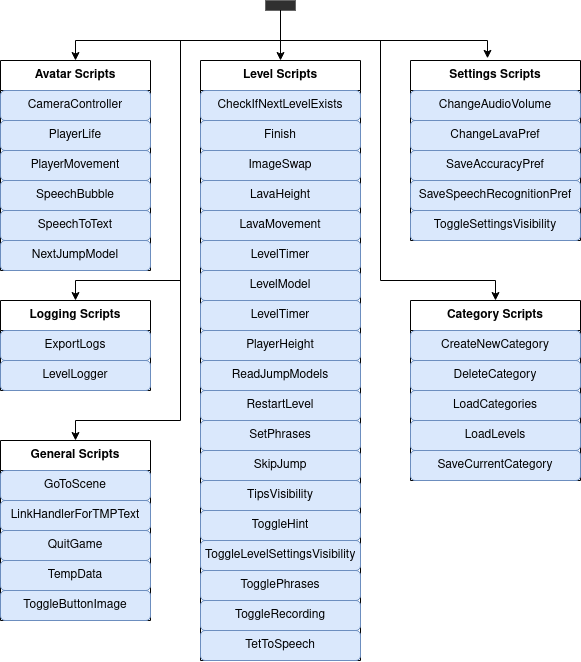
\includegraphics[width=.9\linewidth]{LE_Scripts}
  \caption{Script Structure of the game.}
\end{figure}
\end{comment}

\section{Encountered Problems}
While the current version of the game is already in usage, there are some problems that still need to be addressed in the future. 
\subsection{Voice Recognition}
Even though many improvements during multiple iterations were made, the voice recognition software is still far from optimal. While it excels in interpreting whole words or sentences, it still has trouble detecting single vocals or syllables. Granted, the additional training conducted with the previously gathered test data did somewhat dampen this issue, but it still is far from optimal. The author thus recommends to initially take the following steps if further improvement is needed:
\begin{itemize}
\item \textbf{Gather additional test data}: The data set of single sounds or syllables collected was, while beneficial, still too little. In summary, all 200+ audio files resulted in a total data set size of around 20 MB, which is deemed way too little for neural network training. When collecting more data by enlarging the participant pool, however, one must be cautious that the quality of the single audio files does not deteriorate, i.e., that the sounds are still pronounced correctly. To mitigate this issue within a larger survey setting, it is recommended that speech therapists first voice sample audio files which other participants must first listen to before they can record their own voice. Additionally, limiting the audio collection to proficient participants only can be achieved by contacting multiple schools or therapy centers, for example. Last but not least, providing a monetary incentive or some other kind of benefit is also a viable option if possible. 

\item \textbf{Additional training resources}: Training the neural network was additionally hindered by the absence of training resources for this thesis. This encompasses both the time needed for training and the computing power of the device the network is trained on. For this project, a TUXEDO Sirius 16 with 64 GB of RAM and an AMD Ryzen 7840hs and a training time of around 5 hours was used. It is noteworthy that the training process used was incompatible with the laptop's graphic card, which further halted the training process as all the work had to be done using the device's CPUs only. Thus, the most simple improvement is to employ an NVIDIA graphics card since then the CUDA-API of the training process can be utilized.

\item \textbf{Whisper-Unity bug}: A rather unexpected bug that was found on accident was one related to the Whisper-framework used within Unity. To use the framework, a path to the Whisper image must be provided. However, this path must not contain any special letters (i.e., ä, ö, ü) or it will be interpreted wrongly. This was partly an issue since the therapist wanted to save the game in her logopedics folder which in German is called "Logopädie". This issue could not be fixed as of now, but a bug report describing this issue was posted.
\end{itemize}

\subsection{Export Location}
When the therapist exports logged game data, ideally he or she should be able to choose the logfile's location using a file explorer panel. To implement this feature, Unity's \emph{EditorUtility} class is used in order to open a \emph{Save-File}-window. However, when including this class, the whole game cannot be built anymore. This issue does not appear when playing the game within Unity itself though. As of now, this issue has been mitigated by providing a static location and filename to the export file which is communicated to the therapist beforehand.
\section{Evaluation}
\label{chap:eval}
Once both the therapist and the author were satisfied with the game's development, the next step was to enlarge the testing pool. This process and its result are presented below.

\subsection{Process structure}
For evaluating the game, both author and therapist recruited volunteers wherever feasible. The best recruitment strategies employed were personal communication with friends and relatives, which yielded 15 participants. In contrast, promoting the game on social media (i.e., a Facebook group for local speech therapists) or contacting previously unknown therapists resulted in only four additional participants. This means, that the participants  were either therapists, patients, or volunteers with no logopedical background. In total, 19 people participated in the evaluation process. Regarding the process itself, participants were asked to play the game for at least a month, after which they had to fill out a short questionnaire regarding their experience. Within this month, the participants were also instructed to substitute their usual at-home exercises with playing the game on a regular basis (i.e., 2x per week) if applicable, although the exact frequency was left for them to decide, with the one exception being the one patient that participated. For him, his therapist recommended the frequency. \\
Within the survey following the evaluation period, participants had to answer these therapy-related questions:
\begin{enumerate}
\item Do you believe that Serious Games can be beneficial for speech therapy?
\item How often did you play the game?
\item How much did you like the game (on a scale of 1-10)?
\item How much do you like the classical therapy (on a scale of 1-10)?
\item How much did your speech skills improve by playing the game (on a scale of 1-10)?
\item If you did not play the game in the last weeks, how much would you have improved by doing your usual speech exercises (on a scale of 1-10)?
\item Would you play the game again?
\item Please name one thing you liked about the game (optional).
\item Please name one thing you did not like about the game (optional).
\item What feature would you like to see in future versions (optional)?
\end{enumerate}

These questions were chosen due to both the therapist's recommendation as well as the author's personal intuition. Questions 1,2 and 7 aimed to gather information regarding the general perception of the Serious Game while questions 3,4,5 and 6 were deliberately selected in order to be able to apply the pairwise t-testing methodology on them later on. The last three questions were included in order to gather recommendations which would be relevant for future endeavors.
Furthermore, there were also some additional general questions regarding the participants age, gender and logopedic background. After this quantitative survey was finished, a final interview with the therapist regarding both the state of the current game as well as it's development process was held.

\subsection{Questionnaire results}

In general, participants reacted very positive to the game. Out of the 19 participants, only 15.8\% (n=3) stated that after playing the game for a month they would not consider playing it again whatsoever, though 36.8\% (n=7) said further improvements would have to be made for them to keep playing. However, the field of speech therapy seems to be quite fond of Serious Games altogether as only 2 people stated that they would not consider the inclusion of Serious Games within the therapy process altogether. While this paints quite a positive picture, it does somewhat diminish from this game's evaluation. Nevertheless, for now the result can be considered acceptable. \\
Regarding playing frequency, most participants stated that they have played the game 1-2 times or 3-4 times per week (47.4\% (n=9) and 36.8\% (n=7) respectively). This result was to be expected, as all volunteers were free to choose their own playing frequency. Since for most volunteers playing the game was an addition to their everyday-tasks instead of substituting a different activity, lower frequencies are both more probable and can better be fitted in the volunteer's schedule. However, this is not to be rated negatively as most of the times patients also do not practice on a daily basis \cite{proestler2023}. While daily training might sound to be the most beneficial approach for speech improvement, one must not forget the effects of adequate rest times and steady motivation. Thus, training is often limited to up to four times a week \cite{proestler2023}, with higher frequencies being the exception.\\

Regarding the volunteer's age, 15.8\% (n=3) were between 10-20 years, 47.4\% (n=9) between 20-30, 26.3\% (n=5) between 30-40 and 10.5\% (n=2) between 40-50 years old. This distribution is most likely due to the author's and the therapist's own ages; since both are between 20-30 years of age themselves, it is quite intuitive that they would primarily know people that are roughly around the same age. Next, of the 19 participants 63.2\% (n=12) stated that they were female and 36.8\% (n=7) identified as male. This distribution is not as easily explained as the previous one. Most likely one can assume this distribution to be coincidental and, if more people were to participate, would probably even out more. However, it would also be plausible that a slight tilt towards females would persist as the field of speech therapy is slightly more female-dominated in Austria \cite{LogopedicStatistic}. Nevertheless, the therapy process is not directly affected by this distribution.

\begin{figure}
\begin{subfigure}{.9\textwidth}
  \centering
  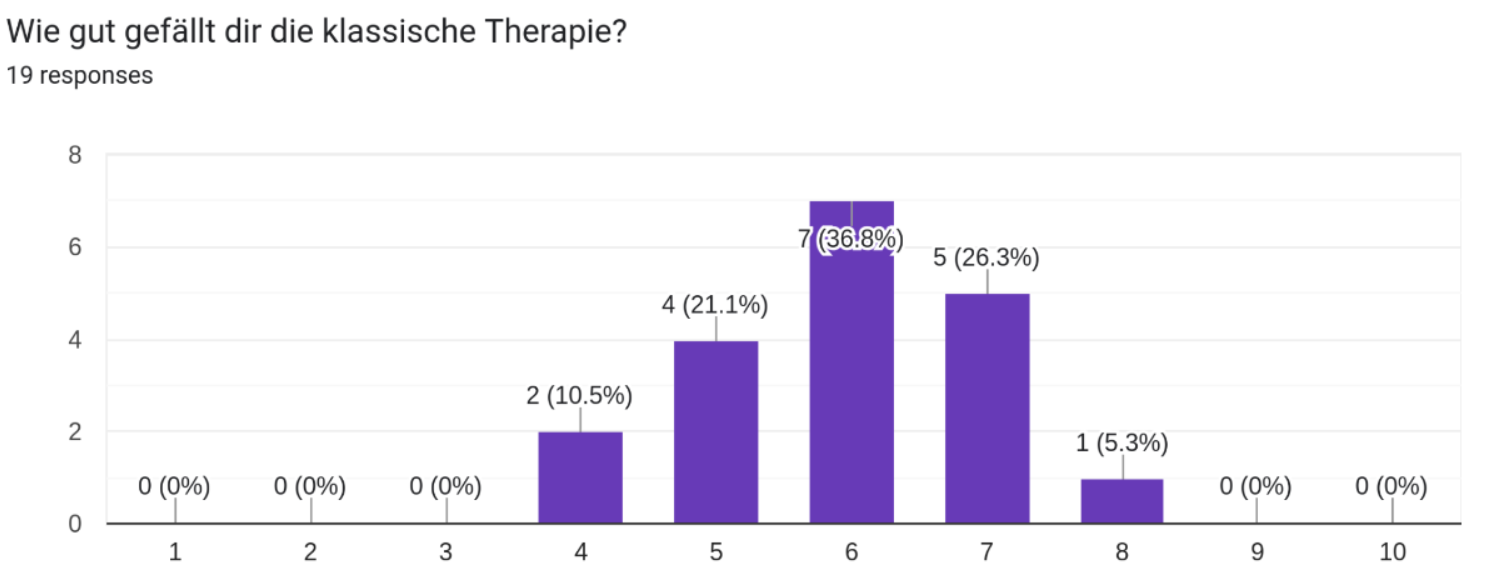
\includegraphics[width=.8\linewidth]{Result_TherapyEnjoyment}
  \caption{Entertainment rating for classical therapy exercises.}
\end{subfigure}
\begin{subfigure}{.9\textwidth}
  \centering
  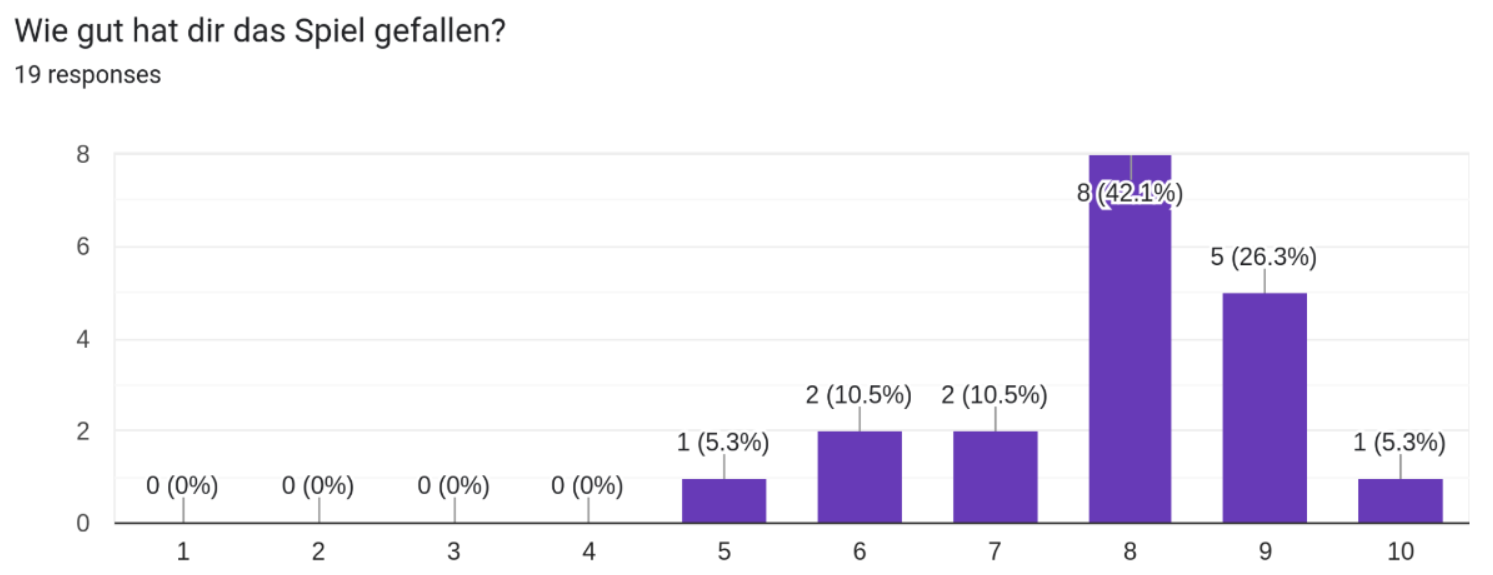
\includegraphics[width=.8\linewidth]{Result_GameEnjoyment}
  \caption{Entertainment rating for the game.}
\end{subfigure}
\caption{Comparison of therapy and game entertainment ratings.}
\end{figure}

Positive results were achieved regarding the game's entertainment measurement, with the average score being 7.89 out of 10. In comparison, the average score for entertainment for classical at-home exercises was measured at 5.95 out of 10.  Using a paired t-test, between these two measurements (with $H_0: m=0$, $p=0.05$) showed that there is a statistical significant difference (mean difference estimation: 1.94 with $p=4.33 \times 10^{-6}$), implying that the perceived entertainment increase provided by the game can be at least further investigated.\\

\begin{figure}
\begin{subfigure}{.9\textwidth}
  \centering
  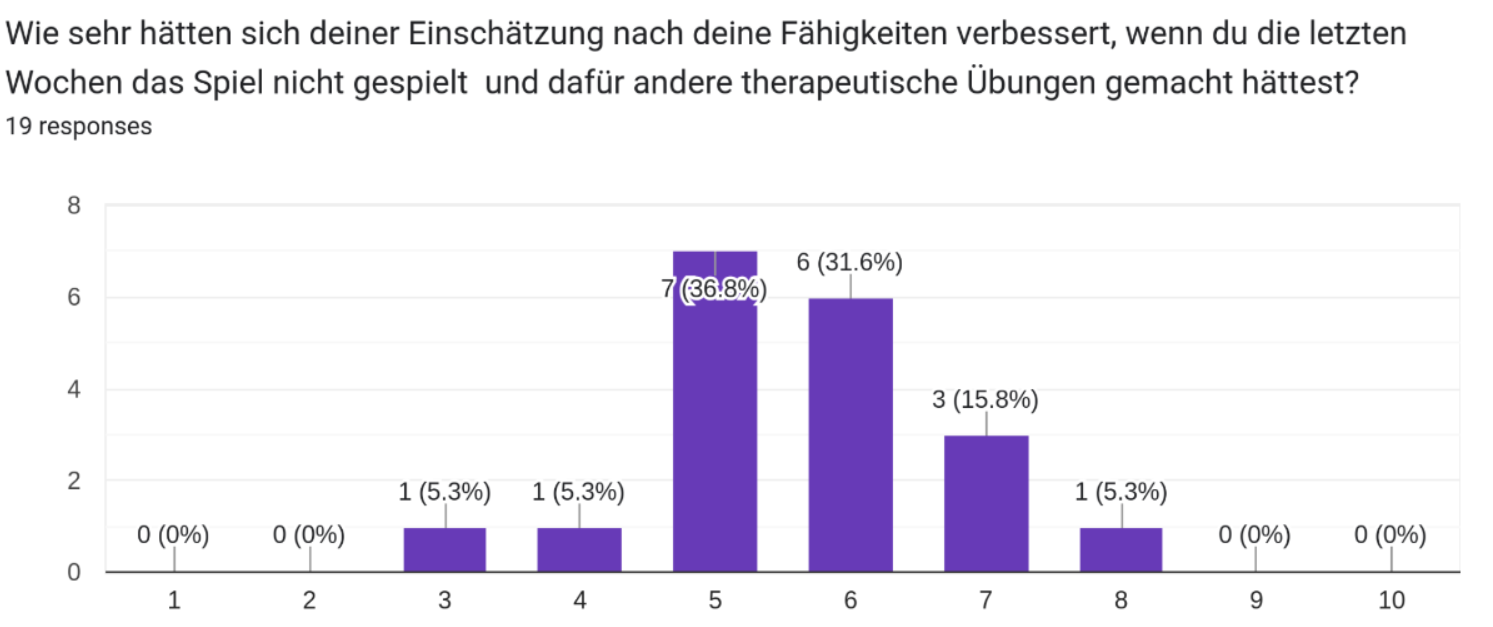
\includegraphics[width=.8\linewidth]{Result_TherapyImprovement}
  \caption{Subjective improvement with classical therapy exercises.}
\end{subfigure}
\begin{subfigure}{.9\textwidth}
  \centering
  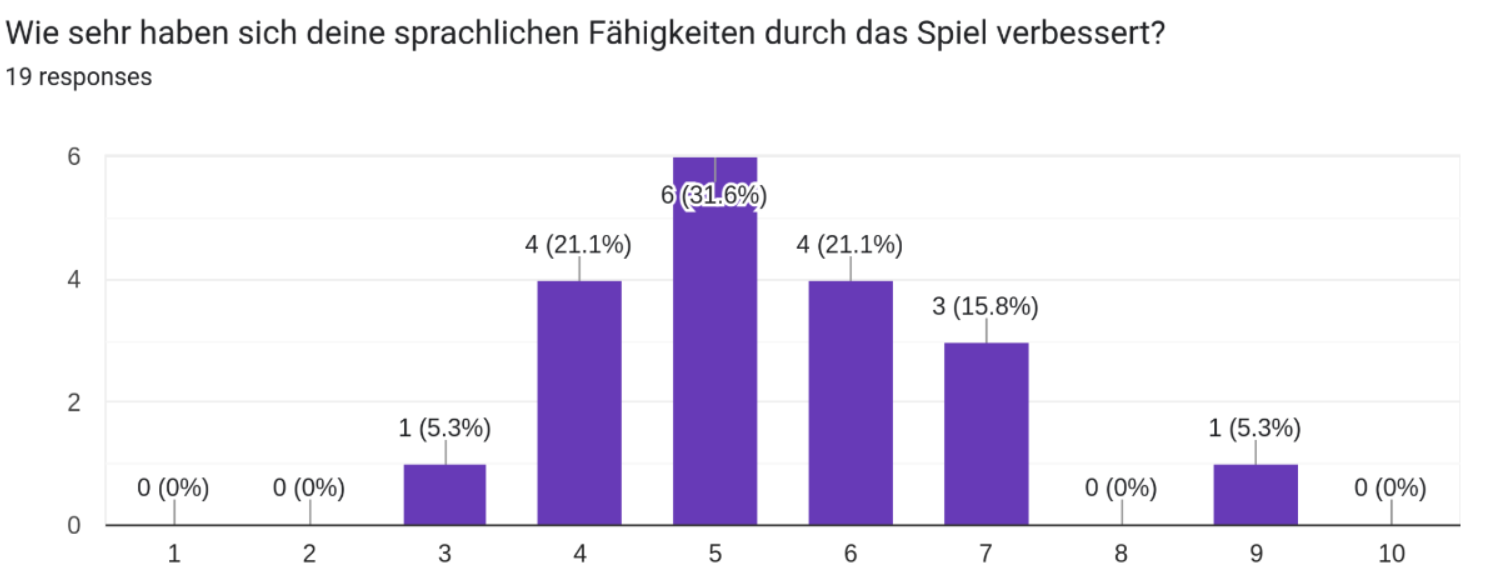
\includegraphics[width=.8\linewidth]{Result_GameImprovement}
  \caption{Subjective improvement for the game.}
\end{subfigure}
\caption{Comparison of subjective improvement between therapy and game.}
\end{figure}

Analyzing the perceived rate of improvement for both the game and alternative at-home exercises, however, resulted in a less favorable outcome. The average score for the game in this regard was measured at 5.42 while therapeutic exercises reached a mean of 5.63. When applying the same paired t-test to these two results, no statistically significant difference could be found (mean difference estimation: 0.21 with $p=0.64$).

\paragraph{Positive feedback} Participants had the option to further elaborate on the game in form of free-text questions.  Players seem to really like the pixel-esque style of the game, mimicking a retro look. Admittedly, the decision to design the game was made in order to save time drawing and animating custom assets so that the developer could put more emphasis on the game's functional features. The fact that this pixelized look has good reception for the volunteers is thus an additional benefit. Next, the main idea (reaching the top) of the game and the game's main playing mechanic (jump via voice) were both positively mentioned. A therapist additionally stated that she liked that logopedical elements (i.e., the progression structure and sound cards) were included in the game as this makes incorporating the game within therapy easier. Last but not least, the level customization editor was a feature that was received very positively since it allowed therapists to tailor the game very well to the patient's therapy goals.

\paragraph{Negative feedback} Almost all negative feedback received were in regards to the quality of the voice recognition feature as it failed to correctly interpret said phrases. Also, the interpretation speed of the voice recognition was mentioned to be too long by one participant, leading to longer waiting times within the game. This issue was known, however, and this feedback was the reason why a toggle option between two different voice recognition components (R29 and R30) were implemented. However, the author hypothesizes that the volunteer who composed this feedback played with the \emph{precise} recognition model, which is more suitable for more performant end devices. Nevertheless, even if that was the case, the option to switch should then at least displayed and labeled more obvious. Additionally, it was mentioned that the Listen-Button (R20) was too quiet and that there was no option to change this, besides from adjusting all sound intensities of the game via the settings-menu.

\paragraph{Additional requested features} If the game were to be updated, participants stated that the following features should be included: 
\begin{itemize}
\item \textbf{Different level backgrounds}: As of now, each level is visually identical, the only exception being the display of exercised phrases. Adding some variety in the form of alternate level backgrounds or platform textures and location makes the game visually more pleasing for a longer time.
\item \textbf{Addition of receptive speech exercises}: While talking is an important part of speech therapy, it is not the only and sometimes not even the optimal way to promote progression. The patient can actually also benefit from just hearing phrases and words. This is something that the current state of the game does not support but was requested by a therapist to be at least considered for future versions. An example within the game could be that in order to advance to the next platform, the player does not have to correctly voice a given word, but rather has to select the right word from a selection of three possibilities depending on what word the game voiced beforehand. If the game were to be developed further after this thesis, this feature will be one of the first to be added.

\item \textbf{Addition of a shop to buy player skins}: By playing the game, players should be awarded with coins which they then can exchange for permanent player skins within an in-game shop. Implementing this feature possibly benefits player motivation and replay value.

\item \textbf{Vocal sound feedback}: Players would like to have the option to hear their last input. This recommendation can help in setting up a better environment (i.e., less interfering noise) and can potentially help the player via self-reflection.

\item \textbf{View game statistics}: A statistics view where players can see the number of levels played, number of inputs voice and the likes should be added. This feature can benefit both patient and therapist at once. 
\end{itemize}

\subsection{Final interview}
As a last step, a final qualitative interview was held with the therapist. The Interview lasted about two hours, although some time was allocated towards a short lunch break. It consisted of 21 open-ended questions which were further classified  into opening questions (i.e., questions regarding the interviewed person),  main questions (i.e., questions regarding the game and development process) and ending questions (i.e., questions that reflect upon the project). While not completely identical, this approach was modeled after a previously established guideline for semi-structured interviews for software project proposed by Weißel \cite{wessel2010semi}. For the full questionnaire, please refer to Section \ref{sec:interview}.

\paragraph{Results of introductory questions} 
As of writing this thesis, the therapist has been treating speech impeded patients for five years. Most of this time she was employed by another more experienced therapist but recently she decided to open up her own office in lower Austria. As most speech therapist, she is capable of helping patients who suffer from speech-, voice,- swallow- or hearing deficiencies. While theoretically she could accept patients of any age, most of them are children between the age of four to six. Depending on the type of impediment at hand, however, she also accepts older patients. An example for this would be patients with braces who suffer from orofacial dysfunction. \\
In most cases, speech therapy lasts about 15 weeks with one session per week. However, depending on the type and severity of the impediment, additional time or practice at home might be required. Since most of her patients are of young age, the therapist aims to incorporate speech exercises within games. As an example, the therapist mentioned playing Ludo but before each dice roll the child has to practice a sound. However, while effective, the therapist mentioned that nowadays children do not enjoy playing classical board games as much as they once did but rather prefer video games instead. This is one reason why the therapist actually agreed to support the author for this thesis in the first place.

\paragraph{Results of main questions}
The main questions were concerned with both the game itself as well as the development process behind it. Regarding the game, the therapist expressed a high degree of satisfaction. She heavily appreciated that her ideas were incorporated into the game to a high degree. Some features she especially mentioned were for example the category editor, the inclusion of logopedical soundcards, the logging capability as a means to track progress and the ability to cover multiple therapy stages. However, similar to the results of the online questionnaire, she did also mention that the game's voice recognition component does not yet perform adequately in both terms of recognition speed and accuracy and, as a result, the game cannot be currently used within therapy. \\
Aside from this issue, however, the therapist responded very positively towards the game. Additionally, she even mentioned some interesting features which can be of interest for future versions. For example, including audio-receptive speech exercise into the game (i.e., the patient does not have to speak themselves but rather has to identify spoken sounds) would be of interest. Also, the possibility to introduce a two-player mode in which the players would either aim to race to the top against each other or to accomplish a common goal cooperative was mentioned. This game mode would be of special interest for parents practicing with their child at home. Last but not least, the therapist also suggested a feature in which submitting one's own list of words to practice would be possible. Ideally, after submitting the list, the game would automatically find or generate fitting sound cards for those words as well. Finally, the therapist voiced that even though she really enjoyed that many of her ideas were incorporated into the game, she believed that the game would benefit even more if other therapists were to provide feedback as well. Sadly, however, all attempts to include other therapists in more depth were not successful. \\
Regarding the project's development process, the therapist expressed that she liked the way the project was conducted. Recurring meetings allowed her to reflect on previous features in more detail as well as gave her time to think about further improvements as well. In total, the development process lasted around 13 months in which a total of six meetings were held, meaning on average one meeting occurred every two months. However, it is worth mentioning that the exact time between meetings was allocated in a more dynamic matter, meaning a meeting was only held if and when it was necessary and promised meaningful improvement afterwards. This flow of development pleased both therapist and author as well as it promoted a creative approach of working on the project. As a last note, the therapist mentioned that if the project were to start anew, the one issue she would like to handle better is to try to contact and incorporate other therapists earlier and with more tenacity.

\paragraph{Results of ending questions}
The last part of the interview consisted of three reflective questions. After the project concluded, the therapist mentioned that she is now more receptive towards inter-professional work and project as participating in this thesis showed her the possibilities such an approach could open. Furthermore, she also enjoyed both sharing knowledge of her domain with the author and also receiving information  from the author's more technical field of expertise. Last but not least, when asked whether she would incorporate Serious Games within therapy in the future she answered that once such games are of sufficient quality, she would not even hesitate to use them. She believes that technology in general will have an ever growing impact in her work and even though Serious Games "will probably not replace speech therapists, it will be able to replace parents", meaning that Serious Games will one day greatly alleviate the parent's responsibility of exercising with their child.

\chapter{Discussion}
\label{chap:discussion}
At the beginning of this thesis, three research questions regarding the analysis, implementation and evaluation of a Serious Game to aid in the speech rehabilitation process were defined. To answer those questions, a prototype of the game and a requirement catalog were created. Afterwards, the game was evaluated by volunteers and their feedback was analyzed. This chapter now presents all three research questions and their outcomes within this thesis.

\section{Research Question 1}
\begin{center}
\emph{What are the requirements towards a Serious Game for speech rehabilitation that can be used across different steps of the rehabilitation process?}
\end{center} 

To answer this question, it is advisable to review the current state of the art. There have already been a multitude of Serious Games for speech rehabilitation before this thesis, analyzing them regarding both their novelties and shortcomings allows for a general first impression regarding the requirements to form. As with any Serious Game, player engagement is crucial as only a played game can benefit the patient. This issue was realized and addressed in many current solutions \cite{Phonak, hair2021longitudinal, navarro2014talking}. Furthermore, reviewing current solutions also helped in identifying missing but wanted features later on during interviews with the speech therapist. In order to better understand the patient's underlying condition, literature research also included an introduction to speech impediments and its variations. A common classification in this regard is made between apraxia (i.e., motoric issues) and aphasia (i.e., speech concept issues) as these two are the most common types of speech impediments addressed within therapy. Within this context, common causes, progression patterns, affected anatomical structures and therapy interventions were discussed. As a result the decision was made to develop a game that only focuses mainly on apraxic patients as such impediments benefit more from a quantitative training approach (i.e., playing the game at home instead of exercising with the therapist). Last but not least, literature research also included a short introduction to the user-centered-design process which was later on used to develop the game in tight collaboration with the therapist. \\

The actual formulated requirements as seen in the requirement catalog were acquired during multiple interview sessions, each taking around 30 to 60 minutes and spanning over a period of around six months. The interviews were held in person at either the therapist's office or at home. One of the first requirements recognized was the ability to use the game over multiple therapy stages as implementing this requirement makes the game longer viable during therapy. Other features that were requested rather quickly were both the alternative sound cards for children and the category customization option. The therapist expressed a high level of delight for the latter one since it allows the game to be adapted for every individual case, rather than presenting a one-size-fits all solution. Additionally, various aiding functionalities like the listen-button were also well received. \\

Starting with the second interview (or second iteration of the UCD-process), each meeting started with showing the current state of the prototype. Issues that were identified in the previous iteration were included in the prototype and shortly showcased to the therapist. Afterwards, the therapist provided feedback to the status quo and recommended additional features to be included. Some features involved the therapist more than others, for example R18 (Pre-defined word list) and R17 (Child Mode) heavily included the therapist. R17 was especially time consuming since each word within the list needs a corresponding sound card. In order to avoid copyright issues, those sound cards were either taken from Madoo \cite{Madoo}, for which the licensing formalities are known, or some sound cards were even drawn by the therapist herself´. Apart from these two requirements, however, the therapist did not implement any features, though her feedback and input were naturally considered and highly valued. Finally, each iteration saw less and less added features but focused more on improving existing ones (i.e., improve feature functionality or make design changes).

In retrospect, while the therapist provided much needed information and highly valuable feedback regarding the game, including patients in early stages of the design process would have resulted in even better results. Issues like replayability and user-engagement for an extended period of time can only be partly addressed by the therapist, who might use the game for half an hour for testing purposes. Having a patient playing the game for an extended period of time, possibly even at home alone, could have been beneficial. Unfortunately, this was not possible due to the therapist's wishes; since the game lacks a robust voice recognition even in its current version, the therapist did not want to recommend it to her patients. Thus the author had to respect the therapist's wishes and continue designing the game with only the therapist as an immediate contributor. Nevertheless, the game's evaluation in phase 3 of this thesis showed that the game has potential use for therapy if current shortcomings are addressed. \\

As a result, a requirement catalog listing all major features needed was created (see Table \ref{tbl:requirements}). While some of those requirements identified can be considered essential for every game (i.e. R6-R10 or R13-R15) and thus arguably do not provide additional research value, most do focus on speech rehabilitation-specific issues. Even then, it could be argued that the requirement catalog is still quite bloated as some requirements could probably be merged together (i.e. R1-R3, R29-R30 or R22-R23). However, the conscious decision to "bloat" this requirement catalog was made so that future work that builds upon this thesis does less likely run into the danger of missing a requirement on accident.


\section{Research Question 2}
\begin{center}
\emph{What logging data within a Serious Game can be used to measure player progress and provide meaningful feedback for speech therapists?}
\end{center} 

For answering this question, the therapist played an integral part. RQ2 was addressed mainly at the beginning of the game design process and only small adaptations were made later on. During interviews with the therapist, a total of four progression metrics that the game can produce were identified. Both \textbf{average sound completion time} (AST) and \textbf{most common mistake} (MCM) were discovered during the first interview. The therapist noted that especially MCM was of interest to her since this metric can be used to indicate what kind of mispronunciation the patient has and can therefore be used to tailor the therapy in more detail. However, while this metric in itself is useful, it heavily relies on the quality of the voice recognition software. While this statement is true for all four metrics, MCM relies the most on it. As previously mentioned, however, the current state of the voice recognition component still has room for improvement, even though significant progress over the course of this thesis was made in this regard. Thus, it is plausible that MCM does not function as intended in the current version of the game. Nevertheless, the idea behind MCM can be considered beneficial for the therapy process and thus should not go unnoticed. During the second interview, the other two progression metrics \textbf{High score: Accuracy} and \textbf{High score: Time} were defined. Both metrics show the player's performance within a higher scope (i.e., whole levels instead of single phrases) and thus are influenced by AST and MCM. Furthermore, the accuracy metric also directly affects the time high score as fewer attempts per phrase usually results in faster completion time. Additionally, the accuracy high score was also used for unlocking new levels as players had to reach a certain accuracy before moving on. All of this data is logged during normal gameplay and can be exported via the main menu. \\

As of now, the above mentioned four metrics were the only ones both the therapist and the author could think of that measure player progress which can be extracted from the game. Other metrics that were up for discussion were for example total playtime, number of levels played or frequency of playing the game. Those metrics, however, do not directly measure player progression but rather show player dedication and adherence to the game. While both dedication and adherence are without a doubt needed for therapy in general and also specifically the game, it does not equal progression. Since RQ2 only addresses player progression metrics, the decision was made to exclude adherence and dedication metrics from the game and alternatively focus on other, more influential features and requirements.

\section{Research Question 3}
\begin{center}
\emph{Does the game provide a subjective benefit within the rehabilitation process for a predefined test group?}
\end{center} 

To answer this question, a playable prototype of the game was developed beforehand and then distributed among testers. The pool of testers mainly consisted of volunteers with no prior connection to speech therapy, but also included multiple therapists and even one patient. While it would have been preferable for all testers to be potential future users of the game this was not possible due to the limited reach of the author and low reply rate to requests sent to therapists. The most effective therapist recruitment strategy was actually implemented by the therapist who helped during the whole thesis. She contacted former study colleagues and current coworkers via WhatsApp and Facebook groups and thus managed to recruit an additional three therapists, one of which even introduced the game to a patient. While the author also made attempts to contact other therapists via E-Mail and phone calls, no additional therapists could be recruited. In total, 19 volunteers agreed to evaluate the game for at least one month after which they answered a short online questionnaire regarding their experience. \\

Analyzing the questionnaire's results gave much insight in the game's current strengths and weaknesses. The most pressing matter was the quality of the voice recognition part which, due to the lack of training data, left room for improvement. This issue was known before distributing the game but since there was no realistic possibility to circumvent it within the scope of this thesis, it was accepted as is. Within the questionnaire, participants had to compare the game with classical therapy exercises patients would do at home regarding two aspects: \textbf{entertainment} and \textbf{improvement}. Regarding entertainment, the results for the game were positive enough that a statistically significant difference was identified, resulting in the conclusion that participants had more fun playing the game as they would have had with doing the therapy exercises. This trend was to be expected for the first week of playing the game since any kind of therapy alternation is initially received well as it provides contrast to the current exercises and are thus new and exciting. However, the fact that the game kept being more entertaining than other exercises even after a whole month of testing indicates a potential long-term increase in entertainment value.  If the game is played for a longer period, this will result in higher patient engagement and thus can even be beneficial towards speech improvement. It should be noted, however, that the questionnaires were mainly filled out by volunteers and not patients, meaning there might not be a clear understanding of what speech therapy exercises are normally done. However, the one patient that participated in the survey also ranked the game higher regarding its entertainment value, thus further supporting the claim. When comparing the subjective rate of improvement that the game and normal at-home exercises had on the participant's speech abilities, no significant difference could be measured. This observation is again to be taken with a grain of salt, as most volunteers never had to exercise at home beforehand and thus had to rely on their own imagination. Including more therapists and especially more patients in future test trials is recommended. Finally, both entertainment and improvement can probably be significantly improved in future versions if the voice recognition component is properly trained by using not only 200, but rather thousands or tens of thousands audio recordings. This statement is meant to highlight that the idea of the game itself as well as its benefit to the patient is probably higher than the questionnaire's results show and the current result is probably tainted by technical limitations. \\

Generally speaking, the field of speech rehabilitation seems to be endorsing the inclusion of Serious Games as most participants (and all therapists and patients) stated that they believe Serious Games can have a positive impact, provided they are developed in collaboration with therapists. However, since the current questionnaire only included five therapy-related participants, further investigation is still needed in the future.
\chapter{Conclusion and future work}
\label{chap:conclusion}
This thesis aimed to design, implement and analyze a Serious Game that can be used within the rehabilitation process of speech-impaired patients. By being mainly interact-able with the use of voice commands, patients are encouraged to practice their speech while playing the game. While the game alone can not completely replace speech therapy, its inclusion aims to ease the learning process at the patient's home. Furthermore, the game also records the player's activity, which can then be viewed by the therapist to measure progression. This chapter summarizes the results of this thesis and provides an outlook to the future regarding the work presented.

\section{Conclusion}
This thesis introduced a Serious Game for patient who are currently undergoing speech therapy. The game heavily builds upon voice recognition in order to provide therapeutic benefit to its players. The field study conducted within this thesis showed high interest in incorporating Serious Games as an additional tool within the speech therapy process. Interviews with one of the participating therapists further support this claim. According to her, especially children are more inclined to play a game than to do repetitive exercises, but adults are likely to benefit as well. Thus, the presented game was developed.\\

The game relies heavily on voice control features. In each level, the player has to issue pre-defined phrases in order to get the avatar to jump from platform to platform until the goal post at the end is reached. Each phrase can be repeated indefinitely until the player issues it correctly. Alternatively, he can skip it after enough attempts. Players who want to challenge themselves more can also enable the lava feature, in which lava slowly rises and once it reaches the avatar, ends the level. Each level can furthermore be customized by the therapist in order to better fit the patient's needs. Last but not least, the game also records the player's activity, which can be viewed and exported by the therapist in order to measure therapy progression. Since the game can be played on multiple platforms (Windows, Linux, Mac or Android), patient accessibility is high and most patients are able include the game within their at-home speech exercise regiment. \\

In order to measure both entertainment and improvement provided by the game, 19 volunteers participated in a field study which ended with them answering a questionnaire. The results showed that the game seems to be more enjoyable than other at-home exercises while having similar subjective speech improvement effects.

\section{Future work}
While this thesis already showed that the inclusion of Serious Games within speech rehabilitation has a high potential, the solution presented is certainly not fully developed and researched yet. During its development, many issues were left untouched due to time and resource restrictions. This last chapter now aims to give some future work suggestions which would further advance on this topic. \\

The final version of the game was evaluated regarding its perceived entertainment and improvement rate with the help of 19 volunteers which evaluated the game for one month and afterwards shared their experience in a questionnaire. However, as already previously mentioned, this evaluation process has some issues which undermine its credibility. The first issue is that most volunteers are not considered to be stakeholders for this game (i.e., therapists or patients) and thus have limited knowledge regarding speech therapy. This naturally makes it difficult for them to compare the game to the therapy which they never underwent. Efforts were made to describe parts of the therapy process, most importantly typical at-home exercises, to the volunteers, but this is not the same as experiencing it yourself. Ideally, the volunteers should consist mainly of patients and some therapists since only they are the ones that potentially use the game afterwards. The second issue is the rather short trial time of one month. Typically, speech therapy spans over months or even years and progress usually does not happen over night. Measuring progress after one month is therefore not reasonable as in most cases only little progress is made overall and thus the difference the game can make in this regard is even smaller. This leads right to the next issue: how exactly should progress be measured? Within this thesis, patients recorded their progress using their own intuition, which is not reliable. If provided resources allow it, a better approach would be to have speech therapists perform standardized tests both before and after the trial period. Furthermore, including a evaluation group which exercises normally for the same duration would further validate whether the game is beneficial as then objectively measurable differences between both approaches would be visible. \\

Regarding the game itself, there is room for improvement as well. The most pressing matter is the speech recognition component as it currently is not precise enough when detecting single sounds or syllables. This issue stems from the fact that currently no voice recognition software focuses on this usage and thus, practically no training data set which only consists of audio files of sounds and syllables exist. This makes training the neural network behind the voice recognition model practically impossible. Within this thesis, an attempt was made to collect fitting audio data from multiple volunteers which resulted in a collection of over 200 audio files, each of which is between one and five seconds long. While this might sound impressive at first, more experienced colleagues working in with neural networks know that this data set is significantly too little and if used for training will most likely result in an overfitted neural network. To further emphasize on this data set gap, consider this: All 200 audio files together take up around 20 MB of space, while usual audio data sets for training contain at least 1GB of data, possibly even 10s or 100s of GB. In conclusion, the author believes that best improvements for the game could be achieved if the training data set would be massively expanded. \\
If resources allow it, this would be done by employing a plethora of volunteers which all provide fitting audio samples. However, since this approach is likely to be quite resource demanding, an alternative solution could be to use existing data sets with audio records that contain whole words or sentences and split them accordingly. That way, multiple sounds and syllables can be extracted from a singular recording, resulting in vast training data. Additionally, the pronunciation of those phrases would be quite authentic since they are literally extracted from whole words. This would make instructing volunteers to fit their pronunciation for provided audio recordings obsolete. However, splitting the audio itself can be quite the difficult task. Since splitting by hand is out of the question due to the massive data size, this process would have to be automated, possibly even AI-driven if necessary. Developing such a solution was not within the scope of this thesis, but promises highly beneficial results.

Another issue that needs addressing is level variability. As of now, each level has the same design, meaning all textures are identical and even the platforms on to which the avatar jumps are in the same position. The only thing that changes from level to level are the required phrases for each jump. Varying both the level's textures as well as platform position could bring more variability into the game and thus keep the player longer engaged. Ideally, levels would be dynamically generated using one of many pre-defined texture sets and adapting platform placement and jump values on the go. Furthermore, the game in general could profit from an extensive UI-overhaul. As of now, the menus and their animations fulfill their purpose, but lack a polished look. Investing additional time and resources into remaking these components would promote the game's appeal substantially. \\

As the evaluation phase showed, the game can also benefit from including additional features. For example, adding an in-game shop where players can trade in-game currency, which they previously collected while playing levels, for alternative skins for their avatars or a different background music could promote adherence. A therapist even suggested adding another playing mode, in which the player does not have to speak himself but rather only hears phrases and afterwards has to correctly guess what they heard from a small predefined selection of options. Another volunteer also suggested adding an audio-replay feature into the game. This would enable the player to hear his last recording and possibly adapt his environment or speech accordingly. Implementing this feature furthermore should be straightforward and thus is an excellent possibility to quickly enhance player satisfaction.\\

Another issue that was not addressed during the prototype is the data log export problem. Selecting a custom destination for the export file is currently only possible when running the game in the Unity Editor, but not when playing the compiled version. This is due to the package that displays the file explorer within the game (\emph{UnityEditor}) conflicts with the build process of the game. It is not yet clear to the author why this occurs but it should be looked into regardless. Last but not least, porting the game for mobile devices (Android or iOS) can also further improve accessibility and should in theory be quite straight-forward as the game does not rely on keyboard input and Unity provides mobile-specific compiling options. Nonetheless adaptions are likely to be necessary in order to provide the best mobile experience.
% Remove following line for the final thesis.
%%% intro.tex
%% Copyright (C) 2014-2020 by Thomas Auzinger <thomas@auzinger.name>
%
% This work may be distributed and/or modified under the
% conditions of the LaTeX Project Public License, either version 1.3
% of this license or (at your option) any later version.
% The latest version of this license is in
%   http://www.latex-project.org/lppl.txt
% and version 1.3 or later is part of all distributions of LaTeX
% version 2005/12/01 or later.
%
% This work has the LPPL maintenance status `maintained'.
%
% The Current Maintainer of this work is Thomas Auzinger.
%
% This work consists of the files vutinfth.dtx and vutinfth.ins
% and the derived file vutinfth.cls.
% This work also consists of the file intro.tex.


\newacronym{ctan}{CTAN}{Comprehensive TeX Archive Network}
\newacronym{faq}{FAQ}{Frequently Asked Questions}
\newacronym{pdf}{PDF}{Portable Document Format}
\newacronym{svn}{SVN}{Subversion}
\newacronym{wysiwyg}{WYSIWYG}{What You See Is What You Get}

\newglossaryentry{texteditor}
{
  name={editor},
  description={A text editor is a type of program used for editing plain text files.}
}

\chapter{Introduction to \LaTeX}

Since \LaTeX\ is widely used in academia and industry, there exists a plethora of freely accessible introductions to the language.
Reading through the guide at \url{https://en.wikibooks.org/wiki/LaTeX} serves as a comprehensive overview for most of the functionality and is highly recommended before starting with a thesis in \LaTeX.

\section{Installation}

A full \LaTeX\ distribution\index{distribution} consists not only of the binaries that convert the source files to the typeset documents, but also of a wide range of packages and their documentation.
Depending on the operating system, different implementations are available as shown in Table~\ref{tab:distrib}.
\textbf{Due to the large amount of packages that are in everyday use and due to their high interdependence, it is paramount to keep the installed distribution\index{distribution} up to date.}
Otherwise, obscure errors and tedious debugging ensue.

\begin{table}
  \centering
  \begin{tabular}{cccc}
    \toprule
    Distribution & Unix         & Windows      & MacOS        \\
    \midrule
    TeX Live     & \textbf{yes} & yes          & (yes)        \\
    MacTeX       & no           & no           & \textbf{yes} \\
    MikTeX       & (yes)        & \textbf{yes} & yes          \\
    \bottomrule
  \end{tabular}
  \caption{\TeX/\LaTeX\ distributions for different operating systems. Recomended choice in \textbf{bold}.}
  \label{tab:distrib} % \label has to be placed AFTER \caption to produce correct cross-references.
\end{table}

\section{Editors}

A multitude of \TeX\ \glspl{texteditor} are available differing in their editing models, their supported operating systems and their feature sets.
A comprehensive overview of \glspl{texteditor} can be found at the Wikipedia page  \url{https://en.wikipedia.org/wiki/Comparison_of_TeX_editors}.
TeXstudio (\url{http://texstudio.sourceforge.net/}) is recommended.
Most editors support a synchronization of the generated document and the \LaTeX\ source by \verb|Ctrl| clicking either on the source document or the generated document.

\section{Compilation}

Modern editors usually provide the compilation programs to generate \gls{pdf} documents and for most \LaTeX\ source files, this is sufficient.
More advanced \LaTeX\ functionality, such as glossaries and bibliographies, needs additional compilation steps, however.
It is also possible that errors in the compilation process invalidate intermediate files and force subsequent compilation runs to fail.
It is advisable to delete intermediate files (\verb|.aux|, \verb|.bbl|, etc.), if errors occur and persist.
All files that are not generated by the user are automatically regenerated.
To compile the current document, the steps as shown in Table~\ref{tab:compile} have to be taken.


\begin{table}
  \centering
  \begin{tabular}{rl}
    \toprule
    & Description \\
    \midrule
    1 & Scan for refs, toc/lof/lot/loa items and cites \\
    2 & Build the bibliography     \\
    3 & Link refs and build the toc/lof/lot/loa \\
    4 & Link the bibliography \\
    5 & Build the glossary \\
    6 & Build the acronyms \\
    7 & Build the index \\
    8 & Link the glossary, acronyms, and the index \\
    9 & Link the bookmarks \\
    \midrule
    & Command \\
    \midrule
    1 & \verb|pdflatex.exe  example| \\
    2 & \verb|bibtex.exe    example| \\
    3 & \verb|pdflatex.exe  example| \\
    4 & \verb|pdflatex.exe  example| \\
    5 & \verb|makeindex.exe -t example.glg -s example.ist| \\
      & \verb|              -o example.gls example.glo| \\
    6 & \verb|makeindex.exe -t example.alg -s example.ist| \\
      & \verb|              -o example.acr example.acn| \\
    7 & \verb|makeindex.exe -t example.ilg -o example.ind example.idx| \\
    8 & \verb|pdflatex.exe  example| \\
    9 & \verb|pdflatex.exe  example| \\
    \bottomrule
  \end{tabular}
  \caption{Compilation steps for this document. The following abbreviations were used: table of contents (toc), list of figures (lof), list of tables (lot), list of algorithms (loa).}
  \label{tab:compile} % \label has to be placed AFTER \caption to produce correct cross-references.
\end{table}


\section{Basic Functionality}

In this section, various examples are given of the fundamental building blocks used in a thesis.
Many \LaTeX\ commands have a rich set of options that can be supplied as optional arguments.
The documentation of each command should be consulted to get an impression of the full spectrum of its functionality.

\subsection{Floats}

Two main categories of page elements can be differentiated in the usual \LaTeX\ workflow: \textit{(i)} the main stream of text and \textit{(ii)} floating containers that are positioned at convenient positions throughout the document.
In most cases, tables, plots, and images are put into such containers since they are usually positioned at the top or bottom of pages.
These are realized by the two environments \verb|figure| and \verb|table|, which also provide functionality for cross-referencing (see Table~\ref{tab:intro} and Figure~\ref{fig:intro}) and the generation of corresponding entries in the list of figures and the list of tables.
Note that these environments solely act as containers and can be assigned arbitrary content.

\subsection{Tables}

A table in \LaTeX\ is created by using a \verb|tabular| environment or any of its extensions, e.g., \verb|tabularx|.
The commands \verb|\multirow| and \verb|\multicolumn| allow table elements to span multiple rows and columns.

\begin{table}[h] % placement specifier
  \centering
  \begin{tabular}{lll}
    \toprule
    \multicolumn{2}{c}{Position} \\
    \cmidrule{1-2} % partial horizontal rule
    Group & Abbrev & Name \\
    \midrule
    Goalkeeper & GK & Paul Robinson \\
    \midrule
    \multirow{4}{*}{Defenders} & LB & Lucus Radebe \\
                               & DC & Michael Duburry \\
                               & DC & Dominic Matteo \\
                               & RB & Didier Domi \\
    \midrule
    \multirow{3}{*}{Midfielders} & MC & David Batty \\
                                 & MC & Eirik Bakke \\
                                 & MC & Jody Morris \\
    \midrule
    Forward & FW & Jamie McMaster \\
    \midrule
    \multirow{2}{*}{Strikers} & ST & Alan Smith \\
                              & ST & Mark Viduka \\
    \bottomrule
  \end{tabular}
  \caption{Adapted example from the \LaTeX guide at \url{https://en.wikibooks.org/wiki/LaTeX/Tables}. This example uses rules specific to the \texttt{booktabs} package and employs the multi-row functionality of the \texttt{multirow} package.}
  \label{tab:intro} % \label has to be placed AFTER \caption to produce correct cross-references.
\end{table}

\subsection{Images}

An image is added to a document via the \verb|\includegraphics| command as shown in Figure~\ref{fig:intro}.
The \verb|\subcaption| command can be used to reference subfigures, such as Figure~\ref{fig:intro:full width} and~\ref{fig:intro:half width}.

\begin{figure}[h]
  \centering
  \begin{subfigure}[b]{0.45\columnwidth}
    \centering
    
\includegraphics[width=\textwidth]{Logo-schwarz.pdf}
    \subcaption{The header logo at text width.}
    \label{fig:intro:full width}
  \end{subfigure}
  \begin{subfigure}[b]{0.45\columnwidth}
    \centering
    
\includegraphics[width=0.5\textwidth]{Logo-schwarz.pdf}
    \subcaption{The header logo at half the text width.}
    \label{fig:intro:half width}
  \end{subfigure}
  \caption[Optional caption for the figure list (often used to abbreviate long captions)]{The header logo at different sizes.} % Remove the [...] argument if the original caption should be used in the figure list.
  \label{fig:intro} % \label has to be placed AFTER \caption (or \subcaption) to produce correct cross-references.
\end{figure}

\subsection{Mathematical Expressions}

One of the original motivation to create the \TeX\ system was the need for mathematical typesetting.
To this day, \LaTeX\ is the preferred system to write math-heavy documents and a wide variety of functions aids the author in this task.
A mathematical expression can be inserted inline as $\sum_{n=1}^{\infty} \frac{1}{n^2} = \frac{\pi^2}{6}$ outside of the text stream as \[ \sum_{n=1}^{\infty} \frac{1}{n^2} = \frac{\pi^2}{6} \] or as numbered equation with
\begin{equation}
\sum_{n=1}^{\infty} \frac{1}{n^2} = \frac{\pi^2}{6}.
\end{equation}

\subsection{Pseudo Code}

The presentation of algorithms can be achieved with various packages; the most popular are \verb|algorithmic|, \verb|algorithm2e|, \verb|algorithmicx|, or \verb|algpseudocode|.
An overview is given at \url{https://tex.stackexchange.com/questions/229355}.
An example of the use of the \verb|alogrithm2e| package is given with Algorithm~\ref{alg:gauss-seidel}.

\begin{algorithm}
  \SetKw{BreakFor}{break for}
  \KwIn{A scalar~$\epsilon$, a matrix $\mathbf{A} = (a_{ij})$, a vector $\vec{b}$, and an initial vector $\vec{x}^{(0)}$}
  \KwOut{$\vec{x}^{(n)}$ with $\mathbf{A} \vec{x}^{(n)} \approx \vec{b}$}
  \For{$k\leftarrow 1$ \KwTo maximum iterations}
  {
     \For{$i\leftarrow 1$ \KwTo $n$}
     {
        $x_i^{(k)} = \frac{1}{a_{ii}} \left(b_i-\sum_{j<i} a_{ij} x_j^{(k)} - \sum_{j>i} a_{ij} x_j^{(k-1)} \right)$\;
     }
     \If{$\lvert\vec{x}^{(k)}-\vec{x}^{(k-1)}\rvert < \epsilon$}
     {\BreakFor\;}
  }
  \Return{$\vec{x}^{(k)}$\;}
  \caption{Gauss-Seidel}
  \label{alg:gauss-seidel} % \label has to be placed AFTER \caption to produce correct cross-references.
\end{algorithm}

\section{Bibliography}

The referencing of prior work is a fundamental requirement of academic writing and well supported by \LaTeX.
The \textsc{Bib}\TeX\ reference management software is the most commonly used system for this purpose.
Using the \verb|\cite| command, it is possible to reference entries in a \verb|.bib| file out of the text stream, e.g., as~\cite{Turing1936}.
The generation of the formatted bibliography needs a separate execution of \verb|bibtex.exe| (see Table~\ref{tab:compile}).

\section{Table of Contents}

The table of contents is automatically built by successive runs of the compilation, e.g., of \verb|pdflatex.exe|.
The command \verb|\setsecnumdepth| allows the specification of the depth of the table of contents and additional entries can be added to the table of contents using \verb|\addcontentsline|.
The starred versions of the sectioning commands, i.e., \verb|\chapter*|, \verb|\section*|, etc., remove the corresponding entry from the table of contents.

\section{Acronyms / Glossary / Index}

The list of acronyms, the glossary, and the index need to be built with a separate execution of \verb|makeindex| (see Table~\ref{tab:compile}).
Acronyms have to be specified with \verb|\newacronym| while glossary entries use \verb|\newglossaryentry|.
Both are then used in the document content with one of the variants of \verb|\gls|, such as \verb|\Gls|, \verb|\glspl|, or \verb|\Glspl|.
Index items are simply generated by placing \verb|\index|\marg{entry} next to all the words that correspond to the index entry \meta{entry}.
Note that many enhancements exist for these functionalities and the documentation of the \verb|makeindex| and the \verb|glossaries| packages should be consulted.

\section{Tips}

Since \TeX\ and its successors do not employ a \gls{wysiwyg} editing scheme, several guidelines improve the readability of the source content:
\begin{itemize}
\item Each sentence in the source text should start with a new line.
      This helps not only the user navigation through the text, but also enables revision control systems (e.g. \gls{svn}, Git) to show the exact changes authored by different users.
      Paragraphs are separated by one (or more) empty lines.
\item Environments, which are defined by a matching pair of \verb|\begin{name}| and \verb|\end{name}|, can be indented by whitespace to show their hierarchical structure.
\item In most cases, the explicit use of whitespace (e.g. by adding \verb|\hspace{4em}| or \verb|\vspace{1.5cm}|) violates typographic guidelines and rules.
      Explicit formatting should only be employed as a last resort and, most likely, better ways to achieve the desired layout can be found by a quick web search.
\item The use of bold or italic text is generally not supported by typographic considerations and the semantically meaningful \verb|\emph{|\texttt{$\dots$}\verb|}| should be used.
\end{itemize}

The predominant application of the \LaTeX\ system is the generation of \gls{pdf} files via the \textsc{Pdf}\LaTeX\ binaries.
In the current version of \textsc{Pdf}\LaTeX, it is possible that absolute file paths and user account names are embedded in the final \gls{pdf} document.
While this poses only a minor security issue for all documents, it is highly problematic for double blind reviews.
The process shown in Table~\ref{tab:ps2pdf} can be employed to strip all private information from the final \gls{pdf} document.

\begin{table}[h]
  \centering
  \begin{tabular}{rl}
  \toprule
  & Command \\
  \midrule
  1 & Rename the \gls{pdf} document \verb|final.pdf| to \verb|final.ps|. \\
  2 & Execute the following command: \\
    & \verb|ps2pdf -dPDFSETTINGS#/prepress ^| \\
    & \verb| -dCompatibilityLevel#1.4 ^| \\
    & \verb| -dAutoFilterColorImages#false ^| \\
    & \verb| -dAutoFilterGrayImages#false ^| \\
    & \verb| -dColorImageFilter#/FlateEncode ^| \\
    & \verb| -dGrayImageFilter#/FlateEncode ^| \\
    & \verb| -dMonoImageFilter#/FlateEncode ^| \\
    & \verb| -dDownsampleColorImages#false ^| \\
    & \verb| -dDownsampleGrayImages#false ^| \\
    & \verb| final.ps final.pdf| \\
  \bottomrule
  \end{tabular}

  On Unix-based systems, replace \verb|#| with \verb|=| and \verb|^| with \verb|\|.
  \caption{Anonymization of \gls{pdf} documents.}
  \label{tab:ps2pdf}
\end{table}

\section{Resources}

\subsection{Useful Links}

In the following, a listing of useful web resources is given.
\begin{description}
\item[\url{https://en.wikibooks.org/wiki/LaTeX}] An extensive wiki-based guide to \LaTeX.
\item[\url{http://www.tex.ac.uk/faq}] A (huge) set of \gls{faq} about \TeX\ and \LaTeX.
\item[\url{https://tex.stackexchange.com/}] The definitive user forum for non-trivial \LaTeX-related questions and answers.
\end{description}

\subsection[Comprehensive TeX Archive Network]{\gls{ctan}}

The \gls{ctan} is the official repository for all \TeX\ related material.
It can be accessed via \url{https://www.ctan.org/} and hosts (among other things) a huge variety of packages that provide extended functionality for \TeX\ and its successors.
Note that most packages contain \gls{pdf} documentation that can be directly accessed via \gls{ctan}.

In the following, a short, non-exhaustive list of relevant \gls{ctan}-hosted packages is given together with their relative path.
\begin{description}[itemsep=0ex]
\item[\href{https://www.ctan.org/pkg/algorithm2e}{algorithm2e}] Functionality for writing pseudo code.
\item[\href{https://www.ctan.org/pkg/amsmath}{amsmath}] Enhanced functionality for typesetting mathematical expressions.
\item[\href{https://www.ctan.org/pkg/amsfonts}{amssymb}] Provides a multitude of mathematical symbols.
\item[\href{https://www.ctan.org/pkg/booktabs}{booktabs}] Improved typesetting of tables.
\item[\href{https://www.ctan.org/pkg/enumitem}{enumitem}] Control over the layout of lists (\verb|itemize|, \verb|enumerate|, \verb|description|).
\item[\href{https://www.ctan.org/pkg/fontenc}{fontenc}] Determines font encoding of the output.
\item[\href{https://www.ctan.org/pkg/glossaries}{glossaries}] Create glossaries and list of acronyms.
\item[\href{https://www.ctan.org/pkg/graphicx}{graphicx}] Insert images into the document.
\item[\href{https://www.ctan.org/pkg/inputenc}{inputenc}] Determines encoding of the input.
\item[\href{https://www.ctan.org/pkg/l2tabu}{l2tabu}] A description of bad practices when using \LaTeX.
\item[\href{https://www.ctan.org/pkg/mathtools}{mathtools}] Further extension of mathematical typesetting.
\item[\href{https://www.ctan.org/pkg/memoir}{memoir}] The document class on upon which the \verb|vutinfth| document class is based.
\item[\href{https://www.ctan.org/pkg/multirow}{multirow}] Allows table elements to span several rows.
\item[\href{https://www.ctan.org/pkg/pgfplots}{pgfplots}] Function plot drawings.
\item[\href{https://www.ctan.org/pkg/pgf}{pgf/TikZ}] Creating graphics inside \LaTeX\ documents.
\item[\href{https://www.ctan.org/pkg/subcaption}{subcaption}] Allows the use of subfigures and enables their referencing.
\item[\href{https://www.ctan.org/tex-archive/info/symbols/comprehensive/}{symbols/comprehensive}] A listing of around 5000 symbols that can be used with \LaTeX.
\item[\href{https://www.ctan.org/pkg/voss-mathmode}{voss-mathmode}] A comprehensive overview of typesetting mathematics in \LaTeX.
\item[\href{https://www.ctan.org/pkg/xcolor}{xcolor}] Allows the definition and use of colors.
\end{description} % A short introduction to LaTeX.

\backmatter

% Use an optional list of figures.
\listoffigures % Starred version, i.e., \listoffigures*, removes the toc entry.

% Use an optional list of tables.
\cleardoublepage % Start list of tables on the next empty right hand page.
\listoftables % Starred version, i.e., \listoftables*, removes the toc entry.

% Use an optional list of alogrithms.
%\listofalgorithms
%\addcontentsline{toc}{chapter}{List of Algorithms}

% Add an index.
%\printindex

% Add a glossary.
%\printglossaries

% Add a bibliography.
\bibliographystyle{unsrt}
\bibliography{intro}

\chapter{Appendix}
\section{Interview Guide}
\label{sec:interview}
Name:\\
Datum: \\

\textbf{Einleitende Fragen}
\begin{enumerate}
\item Beschreibe bitte kurz deinen Werdegang zur Therapeutin.
\item Beschreibe bitte kurz deine Tätigkeit als Therapeutin.
\item Wer ist deine Zielgruppe?
\item Wie läuft eine Therapie bei dir grundsätzlich ab?
\item Welche Mittel verwendest du derzeit in der Therapie?
\end{enumerate}

\textbf{Hauptfragen}
\begin{enumerate}
\item Was hältst du von dem Spiel?
\item Welche Verbesserungen würdest du empfehlen?
\item Welche Verbesserungen wären mindestens nötig, um es deinen Patienten vorzustellen?
\item Was hat dir gut an dem Spiel gefallen?
\item Ist die phasenübergreifende Idee des Spieels (Laute, Silben usw.) deiner Meinung nach gut umgesetzt worden bzw. was würdest du daran ändern?
\item Sollen audiorezeptive Übungen eingebaut werden? Wenn ja wie?
\item Sollen generell andere Spielmodi eingebaut werden?
\item Gibt es sonstige Anmerkungen zu dem Spiel?
\item Wie hat dir der Entwicklungsprozess gefallen?
\item Waren die Meetings in einem adäquaten Zeitabstand oder zu oft/wenig?
\item War dir der Prozess zu strukturiert/unstrukturiert?
\item Wurden deine Wünsche bzw. Empfehlungen ausreichend umgesetzt?
\item Würde das Projekt von Neuem beginnen, was würdest du daran ändern?
\end{enumerate}

\textbf{Schlussfragen}
\begin{enumerate}
\item Was nimmst du aus dem Projekt für dich mit?
\item Wie stehst du nach dem Projekt zu Serious Games in der Sprachrehabilitation?
\item Hast du für dich neue Erkenntnisse gewonnen?
\end{enumerate}
\section{Questionnaire}
  \centering
  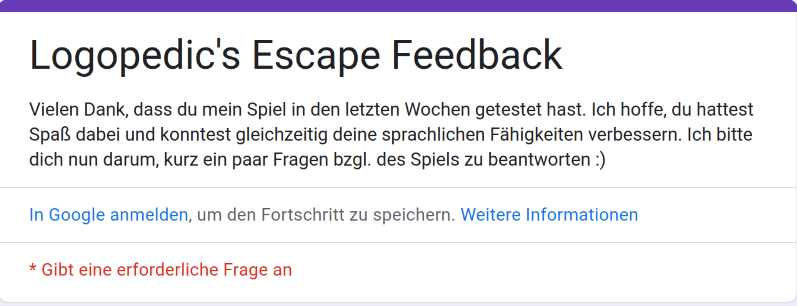
\includegraphics[width=.9\linewidth]{Q1}
  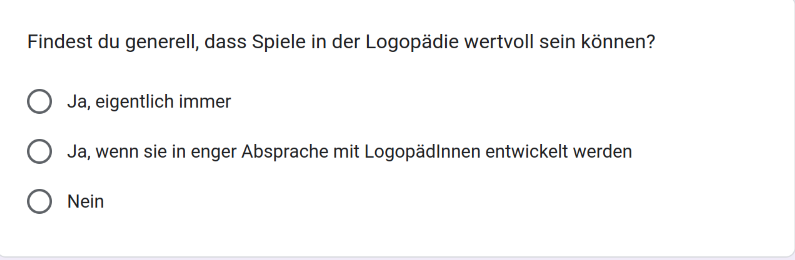
\includegraphics[width=.9\linewidth]{Q2}
  
\includegraphics[width=.9\linewidth]{Q3}
  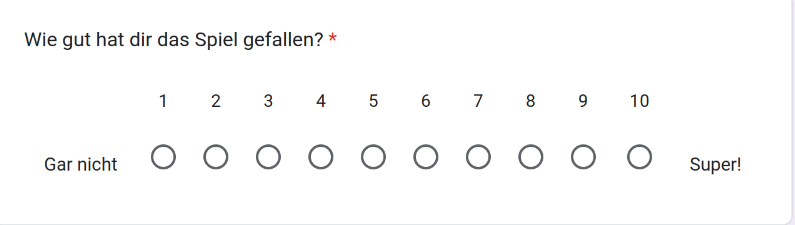
\includegraphics[width=.9\linewidth]{Q4}
  
\includegraphics[width=.9\linewidth]{Q5}
  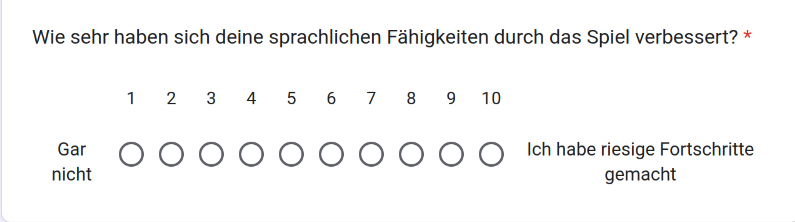
\includegraphics[width=.9\linewidth]{Q6}
  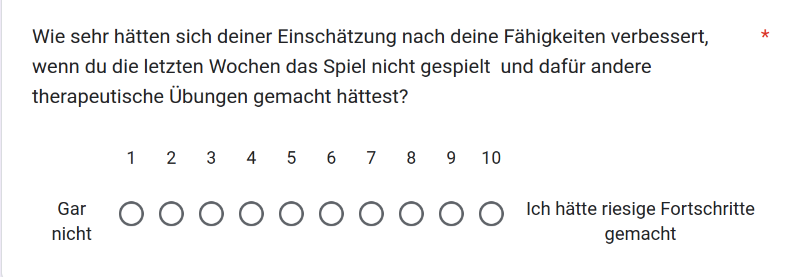
\includegraphics[width=.9\linewidth]{Q7}
  
\includegraphics[width=.9\linewidth]{Q8}
  \includegraphics[width=.9\linewidth]{Q9}
  \includegraphics[width=.9\linewidth]{Q10}
  \includegraphics[width=.9\linewidth]{Q11}
  \includegraphics[width=.9\linewidth]{Q12}
  \includegraphics[width=.9\linewidth]{Q13}
  \includegraphics[width=.9\linewidth]{Q14}
  \includegraphics[width=.9\linewidth]{Q15}
  \includegraphics[width=.9\linewidth]{Q16}
  
\section{Questionnaire results}
  \centering
  \includegraphics[width=.9\linewidth]{Result_valuable}
  \includegraphics[width=.9\linewidth]{Result_frequency}
  \includegraphics[width=.9\linewidth]{Result_GameEnjoyment}
  \includegraphics[width=.9\linewidth]{Result_TherapyEnjoyment}
  \includegraphics[width=.9\linewidth]{Result_GameImprovement}
  \includegraphics[width=.9\linewidth]{Result_TherapyImprovement}
  \includegraphics[width=.9\linewidth]{Result_PlayAgain}
  \includegraphics[width=.9\linewidth]{Result_good}
  \includegraphics[width=.9\linewidth]{Result_bad}
  \includegraphics[width=.9\linewidth]{Result_wish}
  \includegraphics[width=.9\linewidth]{Result_Age}
  \includegraphics[width=.9\linewidth]{Result_Gender}
  \includegraphics[width=.9\linewidth]{Result_Background}


\end{document}
